\documentclass[11pt]{article}

    \usepackage[breakable]{tcolorbox}
    \usepackage{parskip} % Stop auto-indenting (to mimic markdown behaviour)
\usepackage{listings}

\lstset{
    numbers=left,
    numberstyle=\tiny,
    stepnumber=1,
    numbersep=5pt,
    frame=single,
    basicstyle=\ttfamily,
}
    % Basic figure setup, for now with no caption control since it's done
    % automatically by Pandoc (which extracts ![](path) syntax from Markdown).
    \usepackage{graphicx}
    % Maintain compatibility with old templates. Remove in nbconvert 6.0
    \let\Oldincludegraphics\includegraphics
    % Ensure that by default, figures have no caption (until we provide a
    % proper Figure object with a Caption API and a way to capture that
    % in the conversion process - todo).
    \usepackage{caption}
    \usepackage{graphicx}
\usepackage{subfig}
\usepackage{amsmath} % Para el entorno matrix

    \DeclareCaptionFormat{nocaption}{}
    \captionsetup{format=nocaption,aboveskip=0pt,belowskip=0pt}

    \usepackage{float}
    \floatplacement{figure}{H} % forces figures to be placed at the correct location
    \usepackage{xcolor} % Allow colors to be defined
    \usepackage{enumerate} % Needed for markdown enumerations to work
    \usepackage{geometry} % Used to adjust the document margins

    \usepackage{amsmath} % Equations
    \usepackage{amssymb} % Equations
    \usepackage{textcomp} % defines textquotesingle
    % Hack from http://tex.stackexchange.com/a/47451/13684:
    \AtBeginDocument{%
        \def\PYZsq{\textquotesingle}% Upright quotes in Pygmentized code
    }
    \usepackage{upquote} % Upright quotes for verbatim code
    \usepackage{eurosym} % defines \euro

    \usepackage{iftex}
    \ifPDFTeX
        \usepackage[T1]{fontenc}
        \IfFileExists{alphabeta.sty}{
              \usepackage{alphabeta}
          }{
              \usepackage[mathletters]{ucs}
              \usepackage[utf8x]{inputenc}
          }
    \else
        \usepackage{fontspec}
        \usepackage{unicode-math}
    \fi

    \usepackage{fancyvrb} % verbatim replacement that allows latex
    \usepackage{grffile} % extends the file name processing of package graphics
                         % to support a larger range
    \makeatletter % fix for old versions of grffile with XeLaTeX
    \@ifpackagelater{grffile}{2019/11/01}
    {
      % Do nothing on new versions
    }
    {
      \def\Gread@@xetex#1{%
        \IfFileExists{"\Gin@base".bb}%
        {\Gread@eps{\Gin@base.bb}}%
        {\Gread@@xetex@aux#1}%
      }
    }
    \makeatother
    \usepackage[Export]{adjustbox} % Used to constrain images to a maximum size
    \adjustboxset{max size={0.9\linewidth}{0.9\paperheight}}

    % The hyperref package gives us a pdf with properly built
    % internal navigation ('pdf bookmarks' for the table of contents,
    % internal cross-reference links, web links for URLs, etc.)
    \usepackage{hyperref}
    % The default LaTeX title has an obnoxious amount of whitespace. By default,
    % titling removes some of it. It also provides customization options.
    \usepackage{titling}
    \usepackage{longtable} % longtable support required by pandoc >1.10
    \usepackage{booktabs}  % table support for pandoc > 1.12.2
    \usepackage{array}     % table support for pandoc >= 2.11.3
    \usepackage{calc}      % table minipage width calculation for pandoc >= 2.11.1
    \usepackage[inline]{enumitem} % IRkernel/repr support (it uses the enumerate* environment)
    \usepackage[normalem]{ulem} % ulem is needed to support strikethroughs (\sout)
                                % normalem makes italics be italics, not underlines
    \usepackage{soul}      % strikethrough (\st) support for pandoc >= 3.0.0
    \usepackage{mathrsfs}
    

    
    % Colors for the hyperref package
    \definecolor{urlcolor}{rgb}{0,.145,.698}
    \definecolor{linkcolor}{rgb}{.71,0.21,0.01}
    \definecolor{citecolor}{rgb}{.12,.54,.11}

    % ANSI colors
    \definecolor{ansi-black}{HTML}{3E424D}
    \definecolor{ansi-black-intense}{HTML}{282C36}
    \definecolor{ansi-red}{HTML}{E75C58}
    \definecolor{ansi-red-intense}{HTML}{B22B31}
    \definecolor{ansi-green}{HTML}{00A250}
    \definecolor{ansi-green-intense}{HTML}{007427}
    \definecolor{ansi-yellow}{HTML}{DDB62B}
    \definecolor{ansi-yellow-intense}{HTML}{B27D12}
    \definecolor{ansi-blue}{HTML}{208FFB}
    \definecolor{ansi-blue-intense}{HTML}{0065CA}
    \definecolor{ansi-magenta}{HTML}{D160C4}
    \definecolor{ansi-magenta-intense}{HTML}{A03196}
    \definecolor{ansi-cyan}{HTML}{60C6C8}
    \definecolor{ansi-cyan-intense}{HTML}{258F8F}
    \definecolor{ansi-white}{HTML}{C5C1B4}
    \definecolor{ansi-white-intense}{HTML}{A1A6B2}
    \definecolor{ansi-default-inverse-fg}{HTML}{FFFFFF}
    \definecolor{ansi-default-inverse-bg}{HTML}{000000}

    % common color for the border for error outputs.
    \definecolor{outerrorbackground}{HTML}{FFDFDF}

    % commands and environments needed by pandoc snippets
    % extracted from the output of `pandoc -s`
    \providecommand{\tightlist}{%
      \setlength{\itemsep}{0pt}\setlength{\parskip}{0pt}}
    \DefineVerbatimEnvironment{Highlighting}{Verbatim}{commandchars=\\\{\}}
    % Add ',fontsize=\small' for more characters per line
    \newenvironment{Shaded}{}{}
    \newcommand{\KeywordTok}[1]{\textcolor[rgb]{0.00,0.44,0.13}{\textbf{{#1}}}}
    \newcommand{\DataTypeTok}[1]{\textcolor[rgb]{0.56,0.13,0.00}{{#1}}}
    \newcommand{\DecValTok}[1]{\textcolor[rgb]{0.25,0.63,0.44}{{#1}}}
    \newcommand{\BaseNTok}[1]{\textcolor[rgb]{0.25,0.63,0.44}{{#1}}}
    \newcommand{\FloatTok}[1]{\textcolor[rgb]{0.25,0.63,0.44}{{#1}}}
    \newcommand{\CharTok}[1]{\textcolor[rgb]{0.25,0.44,0.63}{{#1}}}
    \newcommand{\StringTok}[1]{\textcolor[rgb]{0.25,0.44,0.63}{{#1}}}
    \newcommand{\CommentTok}[1]{\textcolor[rgb]{0.38,0.63,0.69}{\textit{{#1}}}}
    \newcommand{\OtherTok}[1]{\textcolor[rgb]{0.00,0.44,0.13}{{#1}}}
    \newcommand{\AlertTok}[1]{\textcolor[rgb]{1.00,0.00,0.00}{\textbf{{#1}}}}
    \newcommand{\FunctionTok}[1]{\textcolor[rgb]{0.02,0.16,0.49}{{#1}}}
    \newcommand{\RegionMarkerTok}[1]{{#1}}
    \newcommand{\ErrorTok}[1]{\textcolor[rgb]{1.00,0.00,0.00}{\textbf{{#1}}}}
    \newcommand{\NormalTok}[1]{{#1}}

    % Additional commands for more recent versions of Pandoc
    \newcommand{\ConstantTok}[1]{\textcolor[rgb]{0.53,0.00,0.00}{{#1}}}
    \newcommand{\SpecialCharTok}[1]{\textcolor[rgb]{0.25,0.44,0.63}{{#1}}}
    \newcommand{\VerbatimStringTok}[1]{\textcolor[rgb]{0.25,0.44,0.63}{{#1}}}
    \newcommand{\SpecialStringTok}[1]{\textcolor[rgb]{0.73,0.40,0.53}{{#1}}}
    \newcommand{\ImportTok}[1]{{#1}}
    \newcommand{\DocumentationTok}[1]{\textcolor[rgb]{0.73,0.13,0.13}{\textit{{#1}}}}
    \newcommand{\AnnotationTok}[1]{\textcolor[rgb]{0.38,0.63,0.69}{\textbf{\textit{{#1}}}}}
    \newcommand{\CommentVarTok}[1]{\textcolor[rgb]{0.38,0.63,0.69}{\textbf{\textit{{#1}}}}}
    \newcommand{\VariableTok}[1]{\textcolor[rgb]{0.10,0.09,0.49}{{#1}}}
    \newcommand{\ControlFlowTok}[1]{\textcolor[rgb]{0.00,0.44,0.13}{\textbf{{#1}}}}
    \newcommand{\OperatorTok}[1]{\textcolor[rgb]{0.40,0.40,0.40}{{#1}}}
    \newcommand{\BuiltInTok}[1]{{#1}}
    \newcommand{\ExtensionTok}[1]{{#1}}
    \newcommand{\PreprocessorTok}[1]{\textcolor[rgb]{0.74,0.48,0.00}{{#1}}}
    \newcommand{\AttributeTok}[1]{\textcolor[rgb]{0.49,0.56,0.16}{{#1}}}
    \newcommand{\InformationTok}[1]{\textcolor[rgb]{0.38,0.63,0.69}{\textbf{\textit{{#1}}}}}
    \newcommand{\WarningTok}[1]{\textcolor[rgb]{0.38,0.63,0.69}{\textbf{\textit{{#1}}}}}


    % Define a nice break command that doesn't care if a line doesn't already
    % exist.
    \def\br{\hspace*{\fill} \\* }
    % Math Jax compatibility definitions
    \def\gt{>}
    \def\lt{<}
    \let\Oldtex\TeX
    \let\Oldlatex\LaTeX
    \renewcommand{\TeX}{\textrm{\Oldtex}}
    \renewcommand{\LaTeX}{\textrm{\Oldlatex}}
    % Document parameters
    % Document title
    \title{Untitled6}
    
    
    
    
    
    
    
% Pygments definitions
\makeatletter
\def\PY@reset{\let\PY@it=\relax \let\PY@bf=\relax%
    \let\PY@ul=\relax \let\PY@tc=\relax%
    \let\PY@bc=\relax \let\PY@ff=\relax}
\def\PY@tok#1{\csname PY@tok@#1\endcsname}
\def\PY@toks#1+{\ifx\relax#1\empty\else%
    \PY@tok{#1}\expandafter\PY@toks\fi}
\def\PY@do#1{\PY@bc{\PY@tc{\PY@ul{%
    \PY@it{\PY@bf{\PY@ff{#1}}}}}}}
\def\PY#1#2{\PY@reset\PY@toks#1+\relax+\PY@do{#2}}

\@namedef{PY@tok@w}{\def\PY@tc##1{\textcolor[rgb]{0.73,0.73,0.73}{##1}}}
\@namedef{PY@tok@c}{\let\PY@it=\textit\def\PY@tc##1{\textcolor[rgb]{0.24,0.48,0.48}{##1}}}
\@namedef{PY@tok@cp}{\def\PY@tc##1{\textcolor[rgb]{0.61,0.40,0.00}{##1}}}
\@namedef{PY@tok@k}{\let\PY@bf=\textbf\def\PY@tc##1{\textcolor[rgb]{0.00,0.50,0.00}{##1}}}
\@namedef{PY@tok@kp}{\def\PY@tc##1{\textcolor[rgb]{0.00,0.50,0.00}{##1}}}
\@namedef{PY@tok@kt}{\def\PY@tc##1{\textcolor[rgb]{0.69,0.00,0.25}{##1}}}
\@namedef{PY@tok@o}{\def\PY@tc##1{\textcolor[rgb]{0.40,0.40,0.40}{##1}}}
\@namedef{PY@tok@ow}{\let\PY@bf=\textbf\def\PY@tc##1{\textcolor[rgb]{0.67,0.13,1.00}{##1}}}
\@namedef{PY@tok@nb}{\def\PY@tc##1{\textcolor[rgb]{0.00,0.50,0.00}{##1}}}
\@namedef{PY@tok@nf}{\def\PY@tc##1{\textcolor[rgb]{0.00,0.00,1.00}{##1}}}
\@namedef{PY@tok@nc}{\let\PY@bf=\textbf\def\PY@tc##1{\textcolor[rgb]{0.00,0.00,1.00}{##1}}}
\@namedef{PY@tok@nn}{\let\PY@bf=\textbf\def\PY@tc##1{\textcolor[rgb]{0.00,0.00,1.00}{##1}}}
\@namedef{PY@tok@ne}{\let\PY@bf=\textbf\def\PY@tc##1{\textcolor[rgb]{0.80,0.25,0.22}{##1}}}
\@namedef{PY@tok@nv}{\def\PY@tc##1{\textcolor[rgb]{0.10,0.09,0.49}{##1}}}
\@namedef{PY@tok@no}{\def\PY@tc##1{\textcolor[rgb]{0.53,0.00,0.00}{##1}}}
\@namedef{PY@tok@nl}{\def\PY@tc##1{\textcolor[rgb]{0.46,0.46,0.00}{##1}}}
\@namedef{PY@tok@ni}{\let\PY@bf=\textbf\def\PY@tc##1{\textcolor[rgb]{0.44,0.44,0.44}{##1}}}
\@namedef{PY@tok@na}{\def\PY@tc##1{\textcolor[rgb]{0.41,0.47,0.13}{##1}}}
\@namedef{PY@tok@nt}{\let\PY@bf=\textbf\def\PY@tc##1{\textcolor[rgb]{0.00,0.50,0.00}{##1}}}
\@namedef{PY@tok@nd}{\def\PY@tc##1{\textcolor[rgb]{0.67,0.13,1.00}{##1}}}
\@namedef{PY@tok@s}{\def\PY@tc##1{\textcolor[rgb]{0.73,0.13,0.13}{##1}}}
\@namedef{PY@tok@sd}{\let\PY@it=\textit\def\PY@tc##1{\textcolor[rgb]{0.73,0.13,0.13}{##1}}}
\@namedef{PY@tok@si}{\let\PY@bf=\textbf\def\PY@tc##1{\textcolor[rgb]{0.64,0.35,0.47}{##1}}}
\@namedef{PY@tok@se}{\let\PY@bf=\textbf\def\PY@tc##1{\textcolor[rgb]{0.67,0.36,0.12}{##1}}}
\@namedef{PY@tok@sr}{\def\PY@tc##1{\textcolor[rgb]{0.64,0.35,0.47}{##1}}}
\@namedef{PY@tok@ss}{\def\PY@tc##1{\textcolor[rgb]{0.10,0.09,0.49}{##1}}}
\@namedef{PY@tok@sx}{\def\PY@tc##1{\textcolor[rgb]{0.00,0.50,0.00}{##1}}}
\@namedef{PY@tok@m}{\def\PY@tc##1{\textcolor[rgb]{0.40,0.40,0.40}{##1}}}
\@namedef{PY@tok@gh}{\let\PY@bf=\textbf\def\PY@tc##1{\textcolor[rgb]{0.00,0.00,0.50}{##1}}}
\@namedef{PY@tok@gu}{\let\PY@bf=\textbf\def\PY@tc##1{\textcolor[rgb]{0.50,0.00,0.50}{##1}}}
\@namedef{PY@tok@gd}{\def\PY@tc##1{\textcolor[rgb]{0.63,0.00,0.00}{##1}}}
\@namedef{PY@tok@gi}{\def\PY@tc##1{\textcolor[rgb]{0.00,0.52,0.00}{##1}}}
\@namedef{PY@tok@gr}{\def\PY@tc##1{\textcolor[rgb]{0.89,0.00,0.00}{##1}}}
\@namedef{PY@tok@ge}{\let\PY@it=\textit}
\@namedef{PY@tok@gs}{\let\PY@bf=\textbf}
\@namedef{PY@tok@ges}{\let\PY@bf=\textbf\let\PY@it=\textit}
\@namedef{PY@tok@gp}{\let\PY@bf=\textbf\def\PY@tc##1{\textcolor[rgb]{0.00,0.00,0.50}{##1}}}
\@namedef{PY@tok@go}{\def\PY@tc##1{\textcolor[rgb]{0.44,0.44,0.44}{##1}}}
\@namedef{PY@tok@gt}{\def\PY@tc##1{\textcolor[rgb]{0.00,0.27,0.87}{##1}}}
\@namedef{PY@tok@err}{\def\PY@bc##1{{\setlength{\fboxsep}{\string -\fboxrule}\fcolorbox[rgb]{1.00,0.00,0.00}{1,1,1}{\strut ##1}}}}
\@namedef{PY@tok@kc}{\let\PY@bf=\textbf\def\PY@tc##1{\textcolor[rgb]{0.00,0.50,0.00}{##1}}}
\@namedef{PY@tok@kd}{\let\PY@bf=\textbf\def\PY@tc##1{\textcolor[rgb]{0.00,0.50,0.00}{##1}}}
\@namedef{PY@tok@kn}{\let\PY@bf=\textbf\def\PY@tc##1{\textcolor[rgb]{0.00,0.50,0.00}{##1}}}
\@namedef{PY@tok@kr}{\let\PY@bf=\textbf\def\PY@tc##1{\textcolor[rgb]{0.00,0.50,0.00}{##1}}}
\@namedef{PY@tok@bp}{\def\PY@tc##1{\textcolor[rgb]{0.00,0.50,0.00}{##1}}}
\@namedef{PY@tok@fm}{\def\PY@tc##1{\textcolor[rgb]{0.00,0.00,1.00}{##1}}}
\@namedef{PY@tok@vc}{\def\PY@tc##1{\textcolor[rgb]{0.10,0.09,0.49}{##1}}}
\@namedef{PY@tok@vg}{\def\PY@tc##1{\textcolor[rgb]{0.10,0.09,0.49}{##1}}}
\@namedef{PY@tok@vi}{\def\PY@tc##1{\textcolor[rgb]{0.10,0.09,0.49}{##1}}}
\@namedef{PY@tok@vm}{\def\PY@tc##1{\textcolor[rgb]{0.10,0.09,0.49}{##1}}}
\@namedef{PY@tok@sa}{\def\PY@tc##1{\textcolor[rgb]{0.73,0.13,0.13}{##1}}}
\@namedef{PY@tok@sb}{\def\PY@tc##1{\textcolor[rgb]{0.73,0.13,0.13}{##1}}}
\@namedef{PY@tok@sc}{\def\PY@tc##1{\textcolor[rgb]{0.73,0.13,0.13}{##1}}}
\@namedef{PY@tok@dl}{\def\PY@tc##1{\textcolor[rgb]{0.73,0.13,0.13}{##1}}}
\@namedef{PY@tok@s2}{\def\PY@tc##1{\textcolor[rgb]{0.73,0.13,0.13}{##1}}}
\@namedef{PY@tok@sh}{\def\PY@tc##1{\textcolor[rgb]{0.73,0.13,0.13}{##1}}}
\@namedef{PY@tok@s1}{\def\PY@tc##1{\textcolor[rgb]{0.73,0.13,0.13}{##1}}}
\@namedef{PY@tok@mb}{\def\PY@tc##1{\textcolor[rgb]{0.40,0.40,0.40}{##1}}}
\@namedef{PY@tok@mf}{\def\PY@tc##1{\textcolor[rgb]{0.40,0.40,0.40}{##1}}}
\@namedef{PY@tok@mh}{\def\PY@tc##1{\textcolor[rgb]{0.40,0.40,0.40}{##1}}}
\@namedef{PY@tok@mi}{\def\PY@tc##1{\textcolor[rgb]{0.40,0.40,0.40}{##1}}}
\@namedef{PY@tok@il}{\def\PY@tc##1{\textcolor[rgb]{0.40,0.40,0.40}{##1}}}
\@namedef{PY@tok@mo}{\def\PY@tc##1{\textcolor[rgb]{0.40,0.40,0.40}{##1}}}
\@namedef{PY@tok@ch}{\let\PY@it=\textit\def\PY@tc##1{\textcolor[rgb]{0.24,0.48,0.48}{##1}}}
\@namedef{PY@tok@cm}{\let\PY@it=\textit\def\PY@tc##1{\textcolor[rgb]{0.24,0.48,0.48}{##1}}}
\@namedef{PY@tok@cpf}{\let\PY@it=\textit\def\PY@tc##1{\textcolor[rgb]{0.24,0.48,0.48}{##1}}}
\@namedef{PY@tok@c1}{\let\PY@it=\textit\def\PY@tc##1{\textcolor[rgb]{0.24,0.48,0.48}{##1}}}
\@namedef{PY@tok@cs}{\let\PY@it=\textit\def\PY@tc##1{\textcolor[rgb]{0.24,0.48,0.48}{##1}}}

\def\PYZbs{\char`\\}
\def\PYZus{\char`\_}
\def\PYZob{\char`\{}
\def\PYZcb{\char`\}}
\def\PYZca{\char`\^}
\def\PYZam{\char`\&}
\def\PYZlt{\char`\<}
\def\PYZgt{\char`\>}
\def\PYZsh{\char`\#}
\def\PYZpc{\char`\%}
\def\PYZdl{\char`\$}
\def\PYZhy{\char`\-}
\def\PYZsq{\char`\'}
\def\PYZdq{\char`\"}
\def\PYZti{\char`\~}
% for compatibility with earlier versions
\def\PYZat{@}
\def\PYZlb{[}
\def\PYZrb{]}
\makeatother


    % For linebreaks inside Verbatim environment from package fancyvrb.
    \makeatletter
        \newbox\Wrappedcontinuationbox
        \newbox\Wrappedvisiblespacebox
        \newcommand*\Wrappedvisiblespace {\textcolor{red}{\textvisiblespace}}
        \newcommand*\Wrappedcontinuationsymbol {\textcolor{red}{\llap{\tiny$\m@th\hookrightarrow$}}}
        \newcommand*\Wrappedcontinuationindent {3ex }
        \newcommand*\Wrappedafterbreak {\kern\Wrappedcontinuationindent\copy\Wrappedcontinuationbox}
        % Take advantage of the already applied Pygments mark-up to insert
        % potential linebreaks for TeX processing.
        %        {, <, #, %, $, ' and ": go to next line.
        %        _, }, ^, &, >, - and ~: stay at end of broken line.
        % Use of \textquotesingle for straight quote.
        \newcommand*\Wrappedbreaksatspecials {%
            \def\PYGZus{\discretionary{\char`\_}{\Wrappedafterbreak}{\char`\_}}%
            \def\PYGZob{\discretionary{}{\Wrappedafterbreak\char`\{}{\char`\{}}%
            \def\PYGZcb{\discretionary{\char`\}}{\Wrappedafterbreak}{\char`\}}}%
            \def\PYGZca{\discretionary{\char`\^}{\Wrappedafterbreak}{\char`\^}}%
            \def\PYGZam{\discretionary{\char`\&}{\Wrappedafterbreak}{\char`\&}}%
            \def\PYGZlt{\discretionary{}{\Wrappedafterbreak\char`\<}{\char`\<}}%
            \def\PYGZgt{\discretionary{\char`\>}{\Wrappedafterbreak}{\char`\>}}%
            \def\PYGZsh{\discretionary{}{\Wrappedafterbreak\char`\#}{\char`\#}}%
            \def\PYGZpc{\discretionary{}{\Wrappedafterbreak\char`\%}{\char`\%}}%
            \def\PYGZdl{\discretionary{}{\Wrappedafterbreak\char`\$}{\char`\$}}%
            \def\PYGZhy{\discretionary{\char`\-}{\Wrappedafterbreak}{\char`\-}}%
            \def\PYGZsq{\discretionary{}{\Wrappedafterbreak\textquotesingle}{\textquotesingle}}%
            \def\PYGZdq{\discretionary{}{\Wrappedafterbreak\char`\"}{\char`\"}}%
            \def\PYGZti{\discretionary{\char`\~}{\Wrappedafterbreak}{\char`\~}}%
        }
        % Some characters . , ; ? ! / are not pygmentized.
        % This macro makes them "active" and they will insert potential linebreaks
        \newcommand*\Wrappedbreaksatpunct {%
            \lccode`\~`\.\lowercase{\def~}{\discretionary{\hbox{\char`\.}}{\Wrappedafterbreak}{\hbox{\char`\.}}}%
            \lccode`\~`\,\lowercase{\def~}{\discretionary{\hbox{\char`\,}}{\Wrappedafterbreak}{\hbox{\char`\,}}}%
            \lccode`\~`\;\lowercase{\def~}{\discretionary{\hbox{\char`\;}}{\Wrappedafterbreak}{\hbox{\char`\;}}}%
            \lccode`\~`\:\lowercase{\def~}{\discretionary{\hbox{\char`\:}}{\Wrappedafterbreak}{\hbox{\char`\:}}}%
            \lccode`\~`\?\lowercase{\def~}{\discretionary{\hbox{\char`\?}}{\Wrappedafterbreak}{\hbox{\char`\?}}}%
            \lccode`\~`\!\lowercase{\def~}{\discretionary{\hbox{\char`\!}}{\Wrappedafterbreak}{\hbox{\char`\!}}}%
            \lccode`\~`\/\lowercase{\def~}{\discretionary{\hbox{\char`\/}}{\Wrappedafterbreak}{\hbox{\char`\/}}}%
            \catcode`\.\active
            \catcode`\,\active
            \catcode`\;\active
            \catcode`\:\active
            \catcode`\?\active
            \catcode`\!\active
            \catcode`\/\active
            \lccode`\~`\~
        }
    \makeatother

    \let\OriginalVerbatim=\Verbatim
    \makeatletter
    \renewcommand{\Verbatim}[1][1]{%
        %\parskip\z@skip
        \sbox\Wrappedcontinuationbox {\Wrappedcontinuationsymbol}%
        \sbox\Wrappedvisiblespacebox {\FV@SetupFont\Wrappedvisiblespace}%
        \def\FancyVerbFormatLine ##1{\hsize\linewidth
            \vtop{\raggedright\hyphenpenalty\z@\exhyphenpenalty\z@
                \doublehyphendemerits\z@\finalhyphendemerits\z@
                \strut ##1\strut}%
        }%
        % If the linebreak is at a space, the latter will be displayed as visible
        % space at end of first line, and a continuation symbol starts next line.
        % Stretch/shrink are however usually zero for typewriter font.
        \def\FV@Space {%
            \nobreak\hskip\z@ plus\fontdimen3\font minus\fontdimen4\font
            \discretionary{\copy\Wrappedvisiblespacebox}{\Wrappedafterbreak}
            {\kern\fontdimen2\font}%
        }%

        % Allow breaks at special characters using \PYG... macros.
        \Wrappedbreaksatspecials
        % Breaks at punctuation characters . , ; ? ! and / need catcode=\active
        \OriginalVerbatim[#1,codes*=\Wrappedbreaksatpunct]%
    }
    \makeatother

    % Exact colors from NB
    \definecolor{incolor}{HTML}{303F9F}
    \definecolor{outcolor}{HTML}{D84315}
    \definecolor{cellborder}{HTML}{CFCFCF}
    \definecolor{cellbackground}{HTML}{F7F7F7}

    % prompt
    \makeatletter
    \newcommand{\boxspacing}{\kern\kvtcb@left@rule\kern\kvtcb@boxsep}
    \makeatother
    \newcommand{\prompt}[4]{
        {\ttfamily\llap{{\color{#2}[#3]:\hspace{3pt}#4}}\vspace{-\baselineskip}}
    }
    

    
    % Prevent overflowing lines due to hard-to-break entities
    \sloppy
    % Setup hyperref package
    \hypersetup{
      breaklinks=true,  % so long urls are correctly broken across lines
      colorlinks=true,
      urlcolor=urlcolor,
      linkcolor=linkcolor,
      citecolor=citecolor,
      }
    % Slightly bigger margins than the latex defaults
    
    \geometry{verbose,tmargin=1in,bmargin=1in,lmargin=1in,rmargin=1in}
    
    
% Packages are libraries of commands that LaTeX can call when compiling the document. With the specialized commands you can customize the formatting of your document.
% If the packages we call are not installed yet, TeXworks will ask you to install the necessary packages while compiling.

% First, we usually want to set the margins of our document. For this we use the package geometry. We call the package with the \usepackage command. The package goes in the {}, the parameters again go into the [].
\usepackage[top = 2.5cm, bottom = 2.5cm, left = 0.5cm, right = 2cm]{geometry} 

% Unfortunately, LaTeX has a hard time interpreting German Umlaute. The following two lines and packages should help. If it doesn't work for you please let me know.
\usepackage[T1]{fontenc}
\usepackage[utf8]{inputenc}
\usepackage{siunitx}
\usepackage{enumitem}
\usepackage{amsmath}
\usepackage{listings}
% The following two packages - multirow and booktabs - are needed to create nice looking tables.
\usepackage{multirow} % Multirow is for tables with multiple rows within one cell.
\usepackage{booktabs} % For even nicer tables.

% As we usually want to include some plots (.pdf files) we need a package for that.
\usepackage{graphicx} 

% The default setting of LaTeX is to indent new paragraphs. This is useful for articles. But not really nice for homework problem sets. The following command sets the indent to 0.
\usepackage{setspace}
\setlength{\parindent}{0in}

% Package to place figures where you want them.
\usepackage{float}

% The fancyhdr package let's us create nice headers.
\usepackage{fancyhdr}


%%%%%%%%%%%%%%%%%%%%%%%%%%%%%%%%%%%%%%%%%%%%%%%%
% 3. Header (and Footer)
%%%%%%%%%%%%%%%%%%%%%%%%%%%%%%%%%%%%%%%%%%%%%%%%

% To make our document nice we want a header and number the pages in the footer.

\pagestyle{fancy} % With this command we can customize the header style.

\fancyhf{} % This makes sure we do not have other information in our header or footer.

\lhead{\footnotesize Optimización}% \lhead puts text in the top left corner. \footnotesize sets our font to a smaller size.

%\rhead works just like \lhead (you can also use \chead)
%\rhead{\footnotesize Shickshi Castañeda A. } %<---- Fill in your lastnames.

% Similar commands work for the footer (\lfoot, \cfoot and \rfoot).
% We want to put our page number in the center.
\cfoot{\footnotesize \thepage} 


%%%%%%%%%%%%%%%%%%%%%%%%%%%%%%%%%%%%%%%%%%%%%%%%
% 4. Your document
%%%%%%%%%%%%%%%%%%%%%%%%%%%%%%%%%%%%%%%%%%%%%%%%

% Now, you need to tell LaTeX where your document starts. We do this with the \begin{document} command.
% Like brackets every \begin{} command needs a corresponding \end{} command. We come back to this later.


\begin{document}
    

    
    %%%%%%%%%%%%%%%%%%%%%%%%%%%%%%%%%%%%%%%%%%%%%%%%
%%%%%%%%%%%%%%%%%%%%%%%%%%%%%%%%%%%%%%%%%%%%%%%%

%%%%%%%%%%%%%%%%%%%%%%%%%%%%%%%%%%%%%%%%%%%%%%%%
% Title section of the document
%%%%%%%%%%%%%%%%%%%%%%%%%%%%%%%%%%%%%%%%%%%%%%%%

% For the title section we want to reproduce the title section of the Problem Set and add your names.

\thispagestyle{empty} % This command disables the header on the first page. 

\begin{tabular}{p{15.5cm}} 
{\large \textbf{Curso :} Optimización} \\
Universidad Nacional Mayor de San Marcos \\ Junio 2024  \\
\hline % \hline produces horizontal lines.
\\
\end{tabular} % Our tabular environment ends here.

\vspace*{0.2cm} % Now we want to add some vertical space in between the line and our title.

\begin{center} % Everything within the center environment is centered.
	{\Large \textbf{LISTADO DE EJERCICIOS} \textit{$N^o$} 2} % <---- Don't forget to put in the right number
	\vspace{2mm}
	
        % YOUR NAMES GO HERE
        \begin{center}
%	    {\large Aguilar Morán, Mileynd} \\ 
     \vspace{0.3cm}
            {\large Shickshi Castañeda, Adrian}
            
        \end{center}
		
\end{center}  

\vspace{0.0cm}

%%%%%%%%%%%%%%%%%%%%%%%%%%%%%%%%%%%%%%%%%%%%%%%%
%%%%%%%%%%%%%%%%%%%%%%%%%%%%%%%%%%%%%%%%%%%%%%%%

\section*{Pseudo-Algoritmos}
\[
\begin{cases}
\text{min} \ f(x) \\[2ex]
\text{S.A.}: x \in \mathbb{R}^n
\end{cases}
\]

\begin{lstlisting}
Ingresar:   f(x) ;  x0, error de aproximacion
Salida : Solucion excedida o Numero de intervalos excedido
\end{lstlisting}

\begin{itemize}


    \item Método de gradiente conjugado.
\begin{lstlisting}
PASO 0 :  Dado x0, hacer : 
                g0 = grad(f)(x0)
                d0 = -g0
DETENER SI ||d0|| < Error entonces "x0 es solucion aproximada"

Caso contrario, CONTINUAR:

PASO 1 : Seleccionar t_k(tasa de aprendizaje) usando 
cualquier tipo de estrategia.

                x_{k+1} = x_k+t_k d_{k}
                g_{k+1} == grad(f)(x_{k+1})

SI ||g_{k+1}|| < error, FINALIZAR -> "x_{k+1} solucion optima"

PASO 2 : CASO CONTRARIO : 
                beta_k > 0
                d^{k+1} = -g_{k+1}+beta_k d_{k}
                k <-- k+1
    REGRESAR AL PASO 0
\end{lstlisting}    

\item Método del punto proximal para funciones diferenciables
\begin{lstlisting}
    PASO 0 : Escoger x0 en R^n :
Una sucesion de puntos positivas : t_k > 0

    PASO 1 : Dado k
Si || grad(f)(x_k) || < error -> FINALIZAAR
Caso contrario, seguir :
    
    PASO 2 : Encontrar x^{k+1} en R^{n}
        x^{k+1} = argmin{ f(x)+ t_k / 2 ||x-x^k||^2 , x en R^n }

    PASO 3 : Hacer k <-- k+1 y volver al paso 1
\end{lstlisting}


%Considere : 
%$\longrightarrow$
%\[
%\begin{cases}
%\text{min} \ f(x) = \frac{1}{2} X^T A X - b^T X + C \\[2ex]
%\text{S.A.}: x \in \mathbb{R}^n
%\end{cases}
%\]


%Donde $A \in \mathbb{R}^{n \times n}$
%\\
%\textbf{Def} :
%Dado A $\in S^{n}_{++} =\left\{ X \in \mathbb{R}^{n \times n}, X = X^{T}, X > 0 \right\}, %$ los vectores ${d^0,d^1, \cdots , d^k }$ son A-Conjugados o A - Ortogonales si:
 
\item Método de Newton:

\begin{lstlisting}
    PASO 0 : Dado x_k
SI ||grad(f)(x_k)||< error --> FINALIZAR
CASO CONTRARIO:  

    PASO 1 : RESOLVER
            jacobiano(f)(x^{k}) d = - gradiente(f)(x^{k})
    Un sistema lineal:  d^{k}

    PASO 2: 
            x^{k+1} = x^{k} + t_k d^{k}
Donde t_k > 0; usando cualquier tipo de estrategia 
\end{lstlisting}
Observación : Si la solución está cerca del punto inicial, el método con $t_k = 1$, converge repidamente.

\item Método de Cuasi - Newton\\
Dado un punto inicial $x^o$ y una aproximación de la Hessiana de f, $B_o$ y consideremos $f \in C^{1}(\mathbb{R}^n)$ \\
%  x^{k+1} = x^{k} - t_k (jacobiano(f)(x^{k}) * (grad(f)(x^{k})))    \\ 
\textbf{Actualización Rango 1:}
\[ B_{k+1} = B_{k} + \dfrac{(y_k - B_k s^k)(y_k - B_k s^k)^T}{(y^k - B_k s^k)^T s^k} \]
\textbf{Actualización Rango 2:}
\[ B_{k+1} = B_k - \dfrac{(B_k s^k)(B_k s^k)^T}{s^k B_k s^k} + \dfrac{y^k (y^k)^T}{(y^k)^T s^k}\]
\begin{lstlisting}
    PARA k = 0, 1, 2, ...
    SI x^{k} es un punto critico, PARAR
    CASO CONTRARIO RESOLVER:
            B_{k} d = - graf(f)(x_{k})
    Un sistema lineal:  d^{k}

    REALIZAR UNA BUSQUEDA LINEAL PARA DETERMINAR :
            x^{k+1} = x^{k} + t_k d^{k}

    CALCULAR : 
            s^{k} = x^{k+1} - x^{k}
            y^{k} = grad(f)(x^{k+1}) - grad(f)(x^{k})
            B_{k+1} = B_{k} + ALGO(S^{K},y^{k})

    REGRESAR AL INICIO : 
\end{lstlisting}



\end{itemize}

\section*{Desarrollo : }
\begin{center}
    min\{ $f(x_1,x_2)$ = $e^{-x_1^2-x_2^2} : (x_1,x_2) \in \mathbb{R}^2$\}
\end{center}

\begin{itemize}
    \item Gráfico de curvas de nivel.
    \begin{figure}[h]
    \centering
    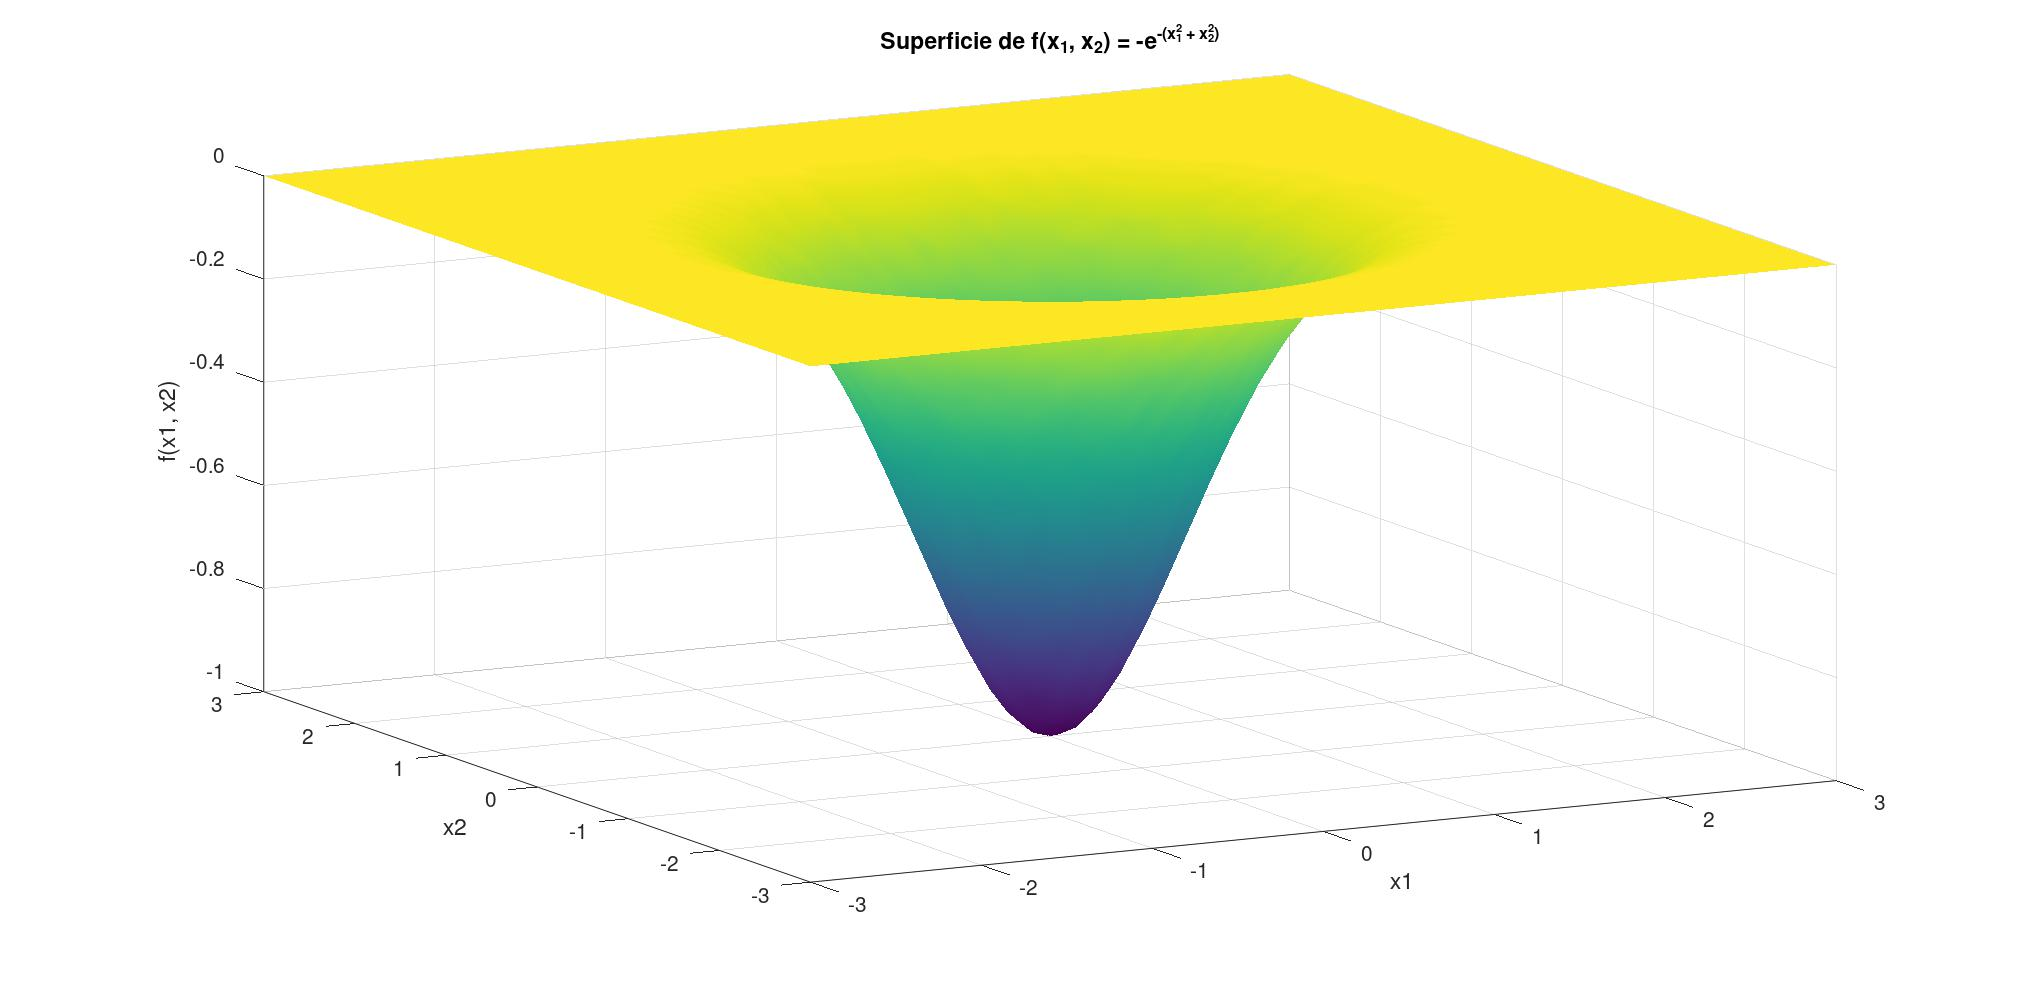
\includegraphics[width=\linewidth]{figuras/grafico.jpg}
\end{figure}

    \item Probar que f es una función cuasi-convexa pero no convexa.
    \section*{Definición de Cuasi-convexidad}

Una función es cuasi-convexa si para todos $x, y$ en su dominio y para todo $\lambda \in [0,1]$, le cumple que:
\[ f(\lambda x + (1-\lambda) y) \geq \min\{f(x), f(y)\} \]

\subsection*{Demostración}

El conjunto de subnivel para un valor $\alpha$ es:
\[ S_\alpha = \{(x_1, x_2) \in \mathbb{R}^2 : f(x_1, x_2) \leq \alpha \} \]

Sea:
\[ f(x_1, x_2) = -e^{x_1^2 - x_2^2} \]

Considerando $\alpha \leq 0$ ($f(x_1, x_2) \leq 0$):
\[ f(x_1, x_2) \leq \alpha \implies -e^{x_1^2 - x_2^2} \leq \alpha \]

Lo cual implica:
\[ e^{-x_1^2 + x_2^2} \geq -\alpha \]
\[ -x_1^2 + x_2^2 \leq \ln(-\alpha) \]
\[ -x_1^2 - x_2^2 \leq \ln(-\alpha) \]
\[ x_2^2 + x_1^2 \leq \ln(-\frac{1}{\alpha}) \]

Dado que los conjuntos de subnivel de $f$ son convexos para cualquier $\alpha \leq 0$, la función $f$ es cuasi-convexa.

\subsection*{Contraejemplo de Convexidad}

Una función $f$ es convexa si para todos $x, y$ en su dominio y para todo $\lambda \in [0,1]$:
\[ f(\lambda x + (1-\lambda) y) \leq \lambda f(x) + (1-\lambda) f(y) \]

Consideremos:
\[ x = (1, 0), \, y = (-1, 0) \]
\[ f(1, 0) = -e^{1^2 - 0^2} = -e^1 = -e \]
\[ f(-1, 0) = -e^{-1^2 - 0^2} = -e^1 = -e \]

Para $\lambda = 0.5$:
\[ \lambda x + (1-\lambda) y = 0.5(1, 0) + 0.5(-1, 0) = (0, 0) \]

Entonces:
\[ f(0, 0) = -e^{0^2 - 0^2} = -e^0 = -1 \]

Comparando:
\[ f(\lambda x + (1-\lambda) y) = f(0, 0) = -1 \]
\[ \lambda f(x) + (1-\lambda) f(y) = 0.5(-e) + 0.5(-e) = -e \]

Como $-1 > -e$, se concluye que la función no es convexa.

    \item Obtener la solución del problema
    Sea la función objetivo:
\[
f(x_1, x_2) = -e^{-x_1^2 - x_2^2}.
\]

\textbf{Paso 1: Calcular las derivadas parciales }

\[
f_{x_1}(x_1, x_2) = \frac{\partial f}{\partial x_1} = -\frac{\partial}{\partial x_1} e^{-x_1^2 - x_2^2}.
\]
\[
\frac{\partial}{\partial x_1} e^{-x_1^2 - x_2^2} = e^{-x_1^2 - x_2^2} \cdot \frac{\partial}{\partial x_1}(-x_1^2 - x_2^2) = e^{-x_1^2 - x_2^2} \cdot (-2x_1).
\]

Por lo tanto,
\[
f_{x_1}(x_1, x_2) = -(-2x_1 e^{-x_1^2 - x_2^2}) = 2x_1 e^{-x_1^2 - x_2^2}.
\]

 Calculando \(f_{x_2}\):
\[
f_{x_2}(x_1, x_2) = \frac{\partial f}{\partial x_2} = -\frac{\partial}{\partial x_2} e^{-x_1^2 - x_2^2} = -(-2x_2 e^{-x_1^2 - x_2^2}) = 2x_2 e^{-x_1^2 - x_2^2}.
\]

\textbf{Paso 2: Resolviendo el sistema de ecuaciones \(\nabla f = 0\)}

Para encontrar los puntos críticos, igualamos las derivadas parciales a cero:
\[
2x_1 e^{-x_1^2 - x_2^2} = 0,
\]
\[
2x_2 e^{-x_1^2 - x_2^2} = 0.
\]

Dado que \(e^{-x_1^2 - x_2^2}\) , debemos tener:
\[
x_1 = 0 \quad \text{y} \quad x_2 = 0.
\]

El único punto crítico es \((x_1, x_2) = (0, 0)\).

\textbf{Paso 3: Verificar la condición de segundo orden}

Calculamos la matriz Hessiana de \(f\):
\[
H_f(x_1, x_2) = \begin{pmatrix}
\frac{\partial^2 f}{\partial x_1^2} & \frac{\partial^2 f}{\partial x_1 \partial x_2} \\
\frac{\partial^2 f}{\partial x_2 \partial x_1} & \frac{\partial^2 f}{\partial x_2^2}
\end{pmatrix}.
\]

Las segundas derivadas son:
\[
f_{x_1 x_1}(x_1, x_2) = \frac{\partial}{\partial x_1} (2x_1 e^{-x_1^2 - x_2^2}) = 2 e^{-x_1^2 - x_2^2} + 2x_1 (-2x_1 e^{-x_1^2 - x_2^2}) = 2 e^{-x_1^2 - x_2^2} (1 - 2x_1^2).
\]

\[
f_{x_2 x_2}(x_1, x_2) = \frac{\partial}{\partial x_2} (2x_2 e^{-x_1^2 - x_2^2}) = 2 e^{-x_1^2 - x_2^2} + 2x_2 (-2x_2 e^{-x_1^2 - x_2^2}) = 2 e^{-x_1^2 - x_2^2} (1 - 2x_2^2).
\]

\[
f_{x_1 x_2}(x_1, x_2) = \frac{\partial}{\partial x_2} (2x_1 e^{-x_1^2 - x_2^2}) = 2x_1 (-2x_2 e^{-x_1^2 - x_2^2}) = -4x_1 x_2 e^{-x_1^2 - x_2^2}.
\]

En \((x_1, x_2) = (0, 0)\), la matriz Hessiana es:
\[
H_f(0, 0) = \begin{pmatrix}
2e^0(1-0) & -4 \cdot 0 \cdot 0 e^0 \\
-4 \cdot 0 \cdot 0 e^0 & 2e^0(1-0)
\end{pmatrix} = \begin{pmatrix}
2 & 0 \\
0 & 2
\end{pmatrix}.
\]

La matriz Hessiana es positiva definida (ambos valores propios son positivos), lo que indica que \((0, 0)\) es un punto de mínimo local.


El mínimo de la función se alcanza en el punto \((x_1, x_2) = (0, 0)\). Evaluando la función en este punto:
\[
f(0, 0) = -e^{-(0)^2 - (0)^2} = -e^0 = -1.
\]

Por lo tanto, el valor mínimo de la función es \(-1\) y ocurre en \((x_1, x_2) = (0, 0)\).
\\

    \item Resultados de aplicar el método de gradiente.

        \begin{itemize}
        \item Utilizando búsqueda unidimensional.

\begin{table}[H]
\centering
\renewcommand{\arraystretch}{1.2} 
\begin{tabular}{|c|c|c|c|c|c|c|}
\hline
\textbf{Iter$_{total}$} &\textbf{x$_{inicial}$} & \textbf{$x^k$} & \textbf{||$\nabla \mathbf{f(x^k)}$}|| & \textbf{f($\mathbf{x^k}$)} &  \textbf{tiempo} \\
\hline
2  &  (0.24 , 0.85) &( 0.0000,0.0000 ) & 0.00000000 & -1.00000000 & 0.2568 \\
2  &  (0.09 , 0.43) &( 0.0000,0.0000 ) & 0.00000000 & -1.00000000 & 0.1800 \\
2  &  (0.85 , 0.12) &( -0.0000,-0.0000 ) & 0.00000000 & -1.00000000 & 0.1790 \\
2  &  (0.34 , 0.15) &( 0.0000,0.0000 ) & 0.00000000 & -1.00000000 & 0.2443 \\
2  &  (0.9 , 0.26) &( 0.0000,0.0000 ) & 0.00000000 & -1.00000000 & 0.2903 \\
2  &  (0.06 , 0.86) &( 0.0000,0.0000 ) & 0.00000000 & -1.00000000 & 0.2665 \\
2  &  (0.59 , 0.78) &( -0.0000,-0.0000 ) & 0.00000000 & -1.00000000 & 0.1710 \\
1  &  (1.9 , 5.49) &( 1.9000,5.4900 ) & 0.00000000 & -0.00000000 & 0.0000 \\
2  &  (1.29 , 2.26) &( -0.0000,-0.0000 ) & 0.00000000 & -1.00000000 & 0.1530 \\
1  &  (2.4 , 3.38) &( 2.4000,3.3800 ) & 0.00000029 & -0.00000003 & 0.0000 \\
1  &  (3.42 , 3.87) &( 3.4200,3.8700 ) & 0.00000000 & -0.00000000 & 0.0000 \\
2  &  (2.46 , 2.07) &( -0.0000,-0.0000 ) & 0.00000000 & -1.00000000 & 0.1562 \\
1  &  (5.65 , 6.18) &( 5.6500,6.1800 ) & 0.00000000 & -0.00000000 & 0.0000 \\
2  &  (2.46 , 2.18) &( 0.0000,0.0000 ) & 0.00000000 & -1.00000000 & 0.1553 \\
2  &  (1.28 , 1.49) &( -0.0000,-0.0000 ) & 0.00000000 & -1.00000000 & 0.2673 \\
2  &  (1.28 , 2.49) &( -0.0000,-0.0000 ) & 0.00000000 & -1.00000000 & 0.2898 \\
1  &  (3.78 , 2.62) &( 3.7800,2.6200 ) & 0.00000001 & -0.00000000 & 0.0000 \\

\hline
\end{tabular}
\end{table}

\begin{figure}
    \centering
    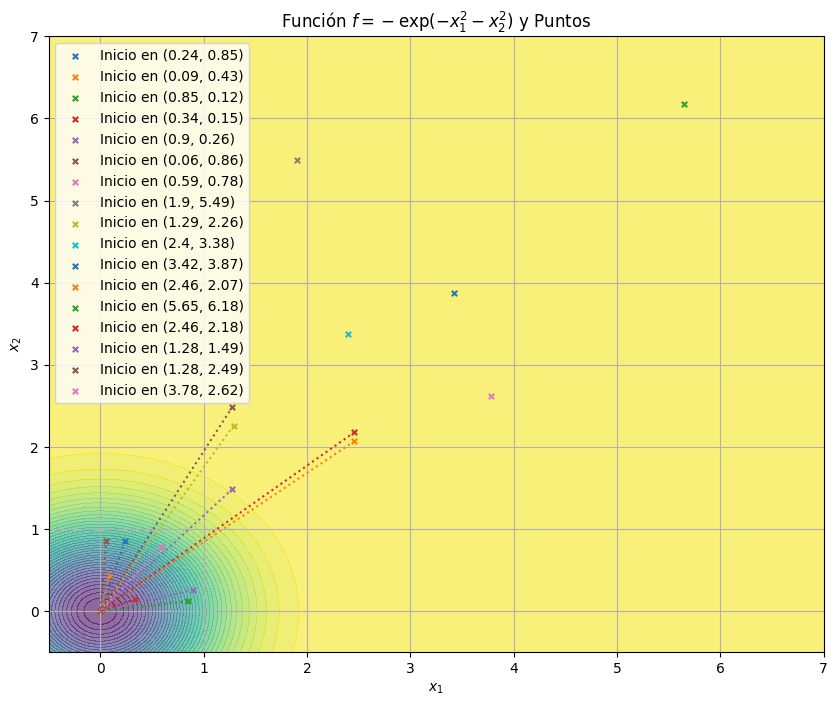
\includegraphics[width=0.73\linewidth]{figuras/PREG4_UNI.png}
    \label{fig:enter-label}
\end{figure}


        \item  Utilizando busqueda de Armijo.
        
\begin{table}[H]
\centering
\renewcommand{\arraystretch}{1.2}
\begin{tabular}{|c|c|c|c|c|c|c|}
\hline
\textbf{It$_{total}$} & \textbf{Arm$_{total}$} & \textbf{$x_{inicial}$} & \textbf{$\mathbf{x^k}$} & \textbf{|| $\nabla$f($\mathbf{x^k}$) ||} & \textbf{f($\mathbf{x^k}$)} & \textbf{tiempo} \\
\hline
3  & 5 &  (0.24 , 0.85) &( 0.0000,0.0000 ) & 0.00000000 & -1.00000000 & 0.0530 \\
3  & 6 &  (0.09 , 0.43) &( 0.0000,0.0000 ) & 0.00000000 & -1.00000000 & 0.0626 \\
3  & 5 &  (0.85 , 0.12) &( 0.0000,0.0000 ) & 0.00000000 & -1.00000000 & 0.0360 \\
3  & 6 &  (0.34 , 0.15) &( 0.0000,0.0000 ) & 0.00000000 & -1.00000000 & 0.0450 \\
3  & 5 &  (0.9 , 0.26) &( 0.0000,0.0000 ) & 0.00000012 & -1.00000000 & 0.0343 \\
3  & 5 &  (0.06 , 0.86) &( 0.0000,0.0000 ) & 0.00000000 & -1.00000000 & 0.0320 \\
5  & 10 &  (0.59 , 0.78) &( 0.0000,0.0000 ) & 0.00000000 & -1.00000000 & 0.0382 \\
0  & 0 &  (1.9 , 5.49) &( 1.9000,5.4900 ) & 0.00000000 & -0.00000000 & 0.0000 \\
45  & 47 &  (1.29 , 2.26) &( -0.0000,-0.0000 ) & 0.00000007 & -1.00000000 & 0.3310 \\
0  & 0 &  (2.4 , 3.38) &( 2.4000,3.3800 ) & 0.00000029 & -0.00000003 & 0.0000 \\
0  & 0 &  (3.42 , 3.87) &( 3.4200,3.8700 ) & 0.00000000 & -0.00000000 & 0.0000 \\
847  & 850 &  (2.46 , 2.07) &( 0.0000,0.0000 ) & 0.00000000 & -1.00000000 & 5.3212 \\
0  & 0 &  (5.65 , 6.18) &( 5.6500,6.1800 ) & 0.00000000 & -0.00000000 & 0.0000 \\
1281  & 1284 &  (2.46 , 2.18) &( 0.0000,0.0000 ) & 0.00000000 & -1.00000000 & 7.3310 \\
9  & 12 &  (1.28 , 1.49) &( 0.0000,0.0000 ) & 0.00000000 & -1.00000000 & 0.0969 \\
102  & 105 &  (1.28 , 2.49) &( 0.0000,0.0000 ) & 0.00000007 & -1.00000000 & 0.5136 \\
0  & 0 &  (3.78 , 2.62) &( 3.7800,2.6200 ) & 0.00000001 & -0.00000000 & 0.0000 \\
\hline
\end{tabular}
\end{table}
Para el gráfico se encuentra lo siguiente:

\begin{itemize}
    \item La trayectoria 8 está vacía.
    \item La trayectoria 10 está vacía.
    \item La trayectoria 11 está vacía.
    \item La trayectoria 13 está vacía.
    \item La trayectoria 17 está vacía.
\end{itemize}



\begin{figure}
    \centering
    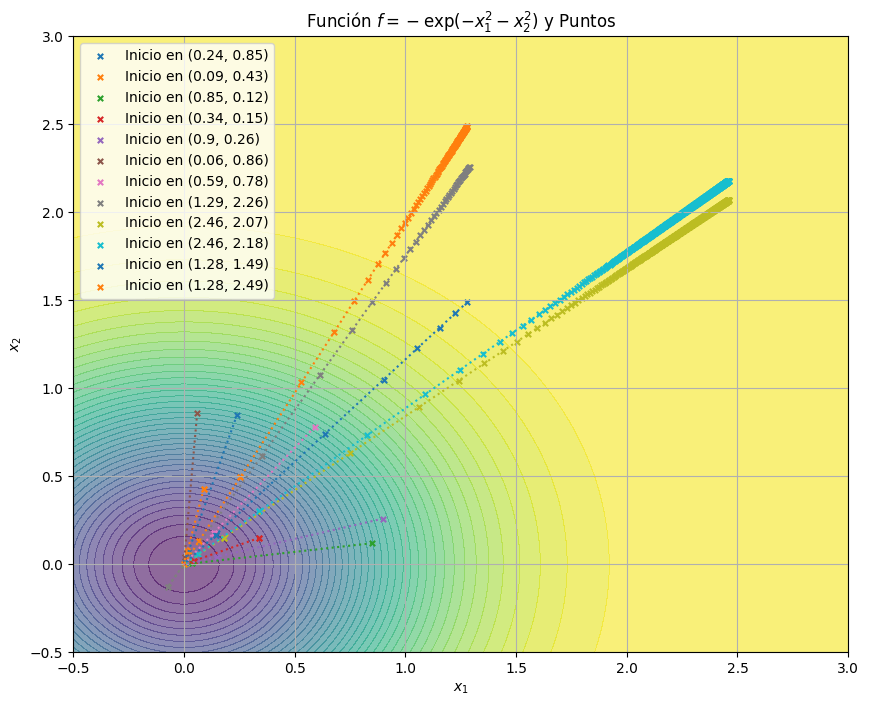
\includegraphics[width=0.75\linewidth]{figuras/PREG4_ARMIJO.png}
    \label{fig:enter-label}
\end{figure}

    \item Resultados de aplicar el método de Newton  con $x_0 =[0.2,0.2]$

    
\begin{itemize}
    \item Newton puro, con : $\lambda_k = 1$
\begin{table}[H]
\centering
\renewcommand{\arraystretch}{1.2} 
\begin{tabular}{|c|c|c|c|c|c|c|}
\hline
\textbf{Iter} & \textbf{$x_{inicial}$} &\textbf{$x^k$} & \textbf{||$\nabla \mathbf{f(x^k)}$}|| & \textbf{f($\mathbf{x^k}$)} & \textbf{tiempo} \\
\hline
5  &  (0.09 , 0.43) &( 0.00000,0.00000 ) & 0.00000000 & -1.00000000 & 0.0577 \\
4  &  (0.34 , 0.15) &( -0.00000,-0.00000 ) & 0.00000084 & -1.00000000 & 0.0449 \\\hline
\end{tabular}
\end{table}

\begin{figure}
    \centering
    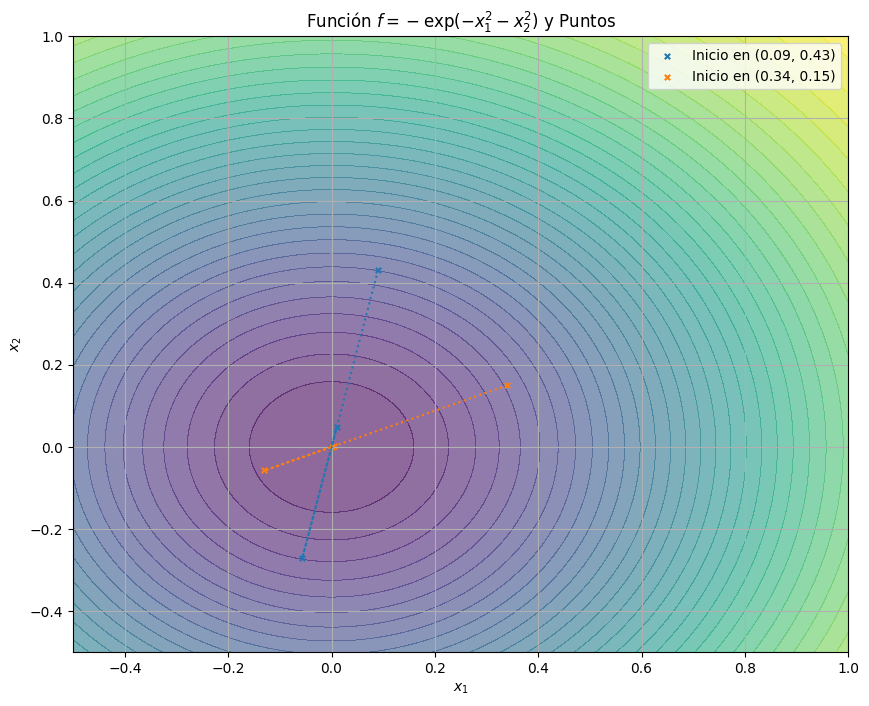
\includegraphics[width=0.65\linewidth]{figuras/PREG5_NEW.png}
    \label{fig:enter-label}
\end{figure}



\begin{itemize}
\item  Hessiana definida no positiva : ( 0.24 ,0.85 )
\item  Hessiana definida no positiva : ( 0.85 ,0.12 )
\item  Hessiana definida no positiva : ( 0.9 ,0.26 )
\item  Hessiana definida no positiva : ( 0.06 ,0.86 )
\item  Hessiana definida no positiva : ( 0.59 ,0.78 )
\item  Hessiana definida no positiva : ( 1.9 ,5.49 )
\item  Hessiana definida no positiva : ( 1.29 ,2.26 )
\item  Hessiana definida no positiva : ( 2.4 ,3.38 )
\item  Hessiana definida no positiva : ( 3.42 ,3.87 )
\item  Hessiana definida no positiva : ( 2.46 ,2.07 )
\item  Hessiana definida no positiva : ( 5.65 ,6.18 )
\item  Hessiana definida no positiva : ( 2.46 ,2.18 )
\item  Hessiana definida no positiva : ( 1.28 ,1.49 )
\item  Hessiana definida no positiva : ( 1.28 ,2.49 )
\item  Hessiana definida no positiva : ( 3.78 ,2.62 )
\end{itemize}









\item Utilizando busqueda exacta.

\begin{table}[H]
\centering
\renewcommand{\arraystretch}{1.2} 
\begin{tabular}{|c|c|c|c|c|c|c|}
\hline
\textbf{Iter} & \textbf{$x_{inicial}$} &\textbf{$x^k$} & \textbf{||$\nabla \mathbf{f(x^k)}$}|| & \textbf{f($\mathbf{x^k}$)} & \textbf{tiempo} \\
\hline
2  &  (0.09 , 0.43) &( 0.00000,0.00000 ) & 0.00000000 & -1.00000000 & 0.2613 \\
2  &  (0.34 , 0.15) &( 0.00000,0.00000 ) & 0.00000000 & -1.00000000 & 0.2652 \\
\hline
\end{tabular}
\end{table}


\begin{figure}
    \centering
    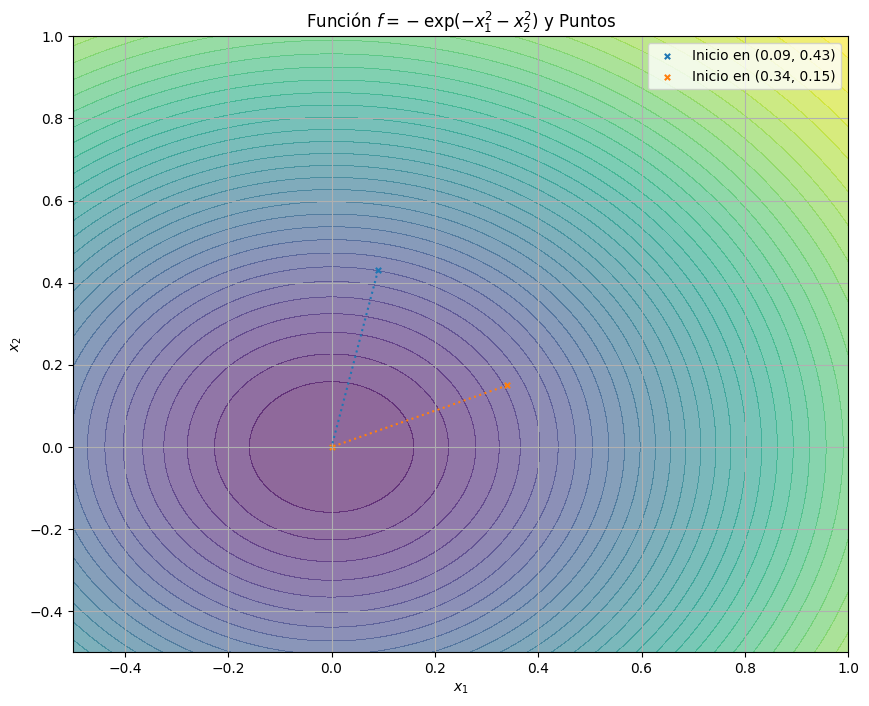
\includegraphics[width=0.65\linewidth]{figuras/PREG5_UNI.png}
    \label{fig:enter-label}
\end{figure}

\item Utilizando busqueda de Armijo


\begin{table}[H]
\centering
\renewcommand{\arraystretch}{1.2}
\begin{tabular}{|c|c|c|c|c|c|c|}
\hline
\textbf{It$_{total}$} & \textbf{Arm$_{total}$} & \textbf{x$_{incial}$} &\textbf{$\mathbf{x^k}$} & \textbf{|| $\nabla$f($\mathbf{x^k}$) ||} & \textbf{f($\mathbf{x^k}$)}&\textbf{tiempo} \\
\hline
14  & 25& (0.09 , 0.43) &( -0.00000,-0.00000 ) & 0.00000000 & -1.00000000 & 0.5776 \\
15  & 27& (0.34 , 0.15) &( -0.00000,-0.00000 ) & 0.00000000 & -1.00000000 & 0.5651 \\
\hline
\end{tabular}
\end{table}
\begin{figure}
    \centering
    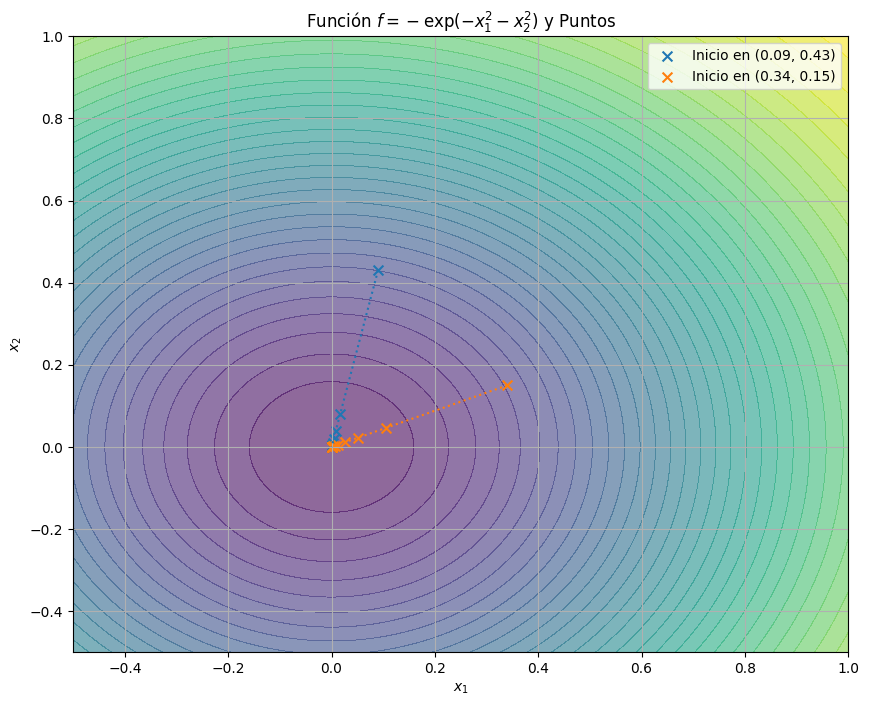
\includegraphics[width=0.65\linewidth]{figuras/PREG5_ARMIJO.png}
    \label{fig:enter-label}
\end{figure}

\end{itemize}





    
    \item Resultados de aplicar el método Cuasi-Newton con actualización de rango 1 y $B =\begin{bmatrix}1&0\\0&1\end{bmatrix}$

    
\begin{itemize}

\item Utilizando busqueda exacta

\begin{table}[H]
\centering
\renewcommand{\arraystretch}{1.2} 
\begin{tabular}{|c|c|c|c|c|c|}
\hline
\textbf{Iter} & \textbf{x$_{inicial}$} & \textbf{$x^k$} & \textbf{||$\nabla \mathbf{f(x^k)}$}|| & \textbf{f($\mathbf{x^k}$)}& \textbf{tiempo} \\
\hline
2  &  (0.24 , 0.85) &( 0.00000,0.00000 ) & 0.00000000 & -1.00000000 & 0.1553 \\
2  &  (0.09 , 0.43) &( 0.00000,0.00000 ) & 0.00000000 & -1.00000000 & 0.1578 \\
2  &  (0.85 , 0.12) &( -0.00000,-0.00000 ) & 0.00000000 & -1.00000000 & 0.1487 \\
2  &  (0.34 , 0.15) &( 0.00000,0.00000 ) & 0.00000000 & -1.00000000 & 0.2452 \\
2  &  (0.9 , 0.26) &( 0.00000,0.00000 ) & 0.00000000 & -1.00000000 & 0.1658 \\
2  &  (0.06 , 0.86) &( 0.00000,0.00000 ) & 0.00000000 & -1.00000000 & 0.2009 \\
2  &  (0.59 , 0.78) &( -0.00000,-0.00000 ) & 0.00000000 & -1.00000000 & 0.1500 \\
1  &  (1.9 , 5.49) &( 1.90000,5.49000 ) & 0.00000000 & -0.00000000 & 0.0000 \\
2  &  (1.29 , 2.26) &( -0.00000,-0.00000 ) & 0.00000000 & -1.00000000 & 0.1339 \\
1  &  (2.4 , 3.38) &( 2.40000,3.38000 ) & 0.00000029 & -0.00000003 & 0.0000 \\
1  &  (3.42 , 3.87) &( 3.42000,3.87000 ) & 0.00000000 & -0.00000000 & 0.0000 \\
2  &  (2.46 , 2.07) &( -0.00000,-0.00000 ) & 0.00000000 & -1.00000000 & 0.1129 \\
1  &  (5.65 , 6.18) &( 5.65000,6.18000 ) & 0.00000000 & -0.00000000 & 0.0000 \\
2  &  (2.46 , 2.18) &( 0.00000,0.00000 ) & 0.00000000 & -1.00000000 & 0.1028 \\
2  &  (1.28 , 1.49) &( -0.00000,-0.00000 ) & 0.00000000 & -1.00000000 & 0.2391 \\
2  &  (1.28 , 2.49) &( -0.00000,-0.00000 ) & 0.00000000 & -1.00000000 & 0.2502 \\
1  &  (3.78 , 2.62) &( 3.78000,2.62000 ) & 0.00000001 & -0.00000000 & 0.0010 \\
\hline
\end{tabular}
\end{table}


\begin{figure}
    \centering
    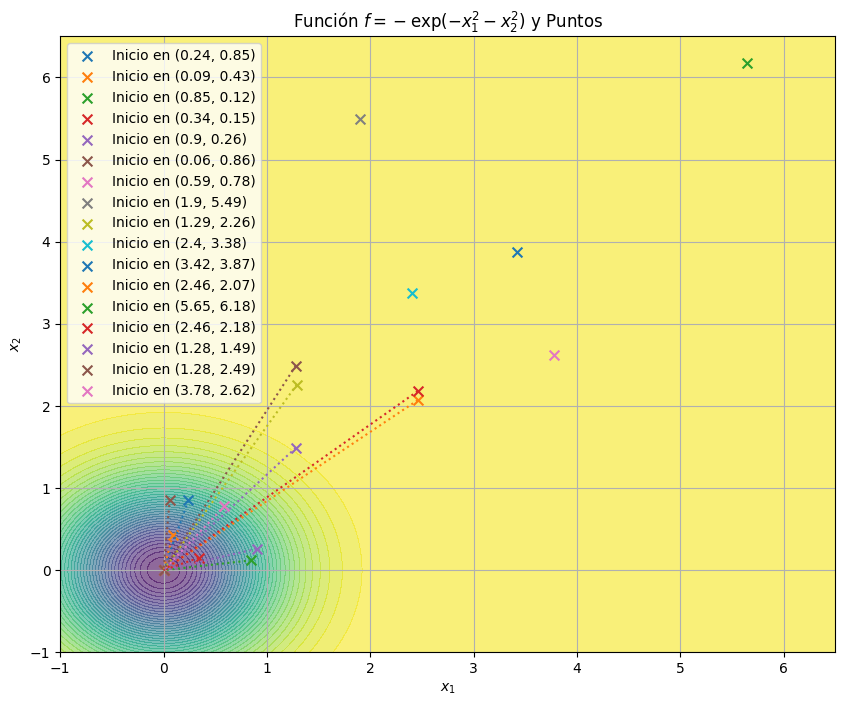
\includegraphics[width=0.65\linewidth]{figuras/PREG6_UNI.png}
    \label{fig:enter-label}
\end{figure}

\item Utilizando busqueda de Armijo


\begin{table}[H]
\centering
\renewcommand{\arraystretch}{1.2}
\begin{tabular}{|c|c|c|c|c|c|c|}
\hline
\textbf{Iter$_{total}$} & \textbf{Arm$_{total}$} &\textbf{x$_{inicial}$}& \textbf{$\mathbf{x^k}$} & \textbf{|| $\nabla$f($\mathbf{x^k}$) ||} & \textbf{f($\mathbf{x^k}$)}  & \textbf{tiempo} \\
\hline
16  &29 & (0.24 , 0.85) &( -0.00000,-0.00000 ) & 0.00000000 & -1.00000000 & 0.1175 \\
13  &23 & (0.09 , 0.43) &( -0.00000,-0.00000 ) & 0.00000000 & -1.00000000 & 0.1534 \\
12  &21 & (0.85 , 0.12) &( -0.00000,-0.00000 ) & 0.00000000 & -1.00000000 & 0.1336 \\
13  &23 & (0.34 , 0.15) &( -0.00000,-0.00000 ) & 0.00000000 & -1.00000000 & 0.1534 \\
16  &29 & (0.9 , 0.26) &( -0.00000,-0.00000 ) & 0.00000000 & -1.00000000 & 0.2129 \\
15  &27 & (0.06 , 0.86) &( -0.00000,-0.00000 ) & 0.00000000 & -1.00000000 & 0.2155 \\
16  &30 & (0.59 , 0.78) &( -0.00000,-0.00000 ) & 0.00000000 & -1.00000000 & 0.2456 \\
1  &0 & (1.9 , 5.49) &( 1.90000,5.49000 ) & 0.00000000 & -0.00000000 & 0.0000 \\
\hline
\end{tabular}
\end{table}

\begin{figure}
    \centering
    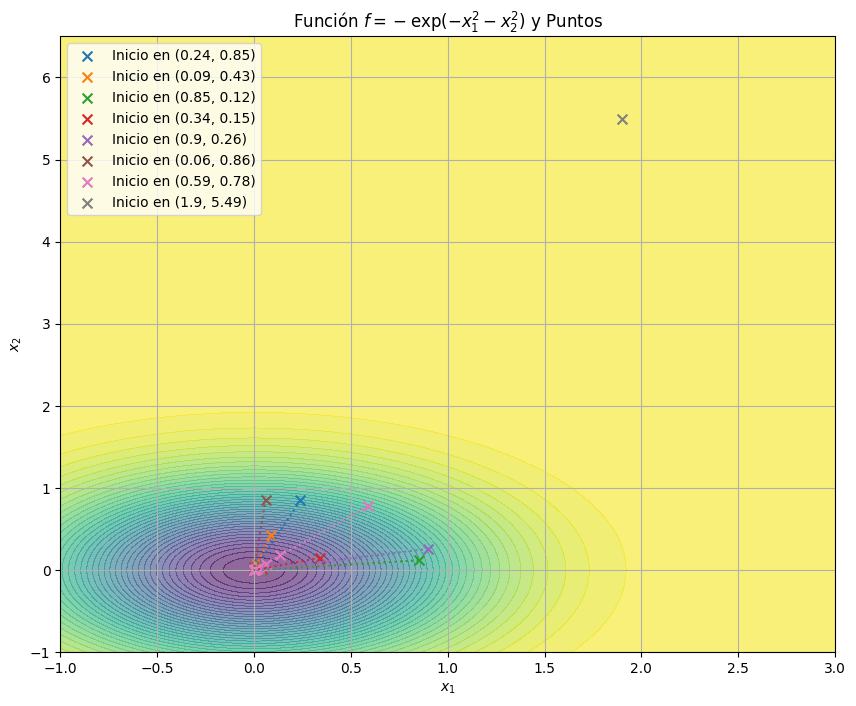
\includegraphics[width=0.65\linewidth]{figuras/PREG6_ARMIJO.png}
    \label{fig:enter-label}
\end{figure}

\end{itemize}





    
    \item Resultados de aplicar el método de gradiente conjugado, considerando: $\beta_k = 0.2$

    \begin{itemize}

\item Utilizando busqueda exacta

\begin{table}[H]
\centering
\renewcommand{\arraystretch}{1.2}
\begin{tabular}{|c|c|c|c|c|c|c|}
\hline
\textbf{Iter} & \textbf{x$_{inicial}$}& \textbf{$x^k$} & \textbf{||$\nabla \mathbf{f(x^k)}$}|| & \textbf{f($\mathbf{x^k}$)}& \textbf{tiempo} \\
\hline
1  & (0.24 , 0.85) &( 0.00000,0.00000 ) & 0.00000000 & -1.00000000 & 0.2270 \\
1  & (0.09 , 0.43) &( 0.00000,0.00000 ) & 0.00000000 & -1.00000000 & 0.1866 \\
1  & (0.85 , 0.12) &( -0.00000,-0.00000 ) & 0.00000000 & -1.00000000 & 0.2022 \\
1  & (0.34 , 0.15) &( 0.00000,0.00000 ) & 0.00000000 & -1.00000000 & 0.2721 \\
1  & (0.9 , 0.26) &( 0.00000,0.00000 ) & 0.00000000 & -1.00000000 & 0.2483 \\
1  & (0.06 , 0.86) &( 0.00000,0.00000 ) & 0.00000000 & -1.00000000 & 0.2233 \\
1  & (0.59 , 0.78) &( -0.00000,-0.00000 ) & 0.00000000 & -1.00000000 & 0.1480 \\
1  & (1.9 , 5.49) &( 1.90000,5.49000 ) & 0.00000000 & -0.00000000 & 0.0000 \\
1  & (1.29 , 2.26) &( -0.00000,-0.00000 ) & 0.00000000 & -1.00000000 & 0.1238 \\
1  & (2.4 , 3.38) &( 2.40000,3.38000 ) & 0.00000029 & -0.00000003 & 0.0000 \\
1  & (3.42 , 3.87) &( 3.42000,3.87000 ) & 0.00000000 & -0.00000000 & 0.0000 \\
1  & (2.46 , 2.07) &( -0.00000,-0.00000 ) & 0.00000000 & -1.00000000 & 0.1105 \\
1  & (5.65 , 6.18) &( 5.65000,6.18000 ) & 0.00000000 & -0.00000000 & 0.0000 \\
1  & (2.46 , 2.18) &( 0.00000,0.00000 ) & 0.00000000 & -1.00000000 & 0.1035 \\
1  & (1.28 , 1.49) &( -0.00000,-0.00000 ) & 0.00000000 & -1.00000000 & 0.1800 \\
1  & (1.28 , 2.49) &( -0.00000,-0.00000 ) & 0.00000000 & -1.00000000 & 0.1685 \\
1  & (3.78 , 2.62) &( 3.78000,2.62000 ) & 0.00000001 & -0.00000000 & 0.0000 \\
\hline
\end{tabular}
\end{table}

\begin{figure}
    \centering
    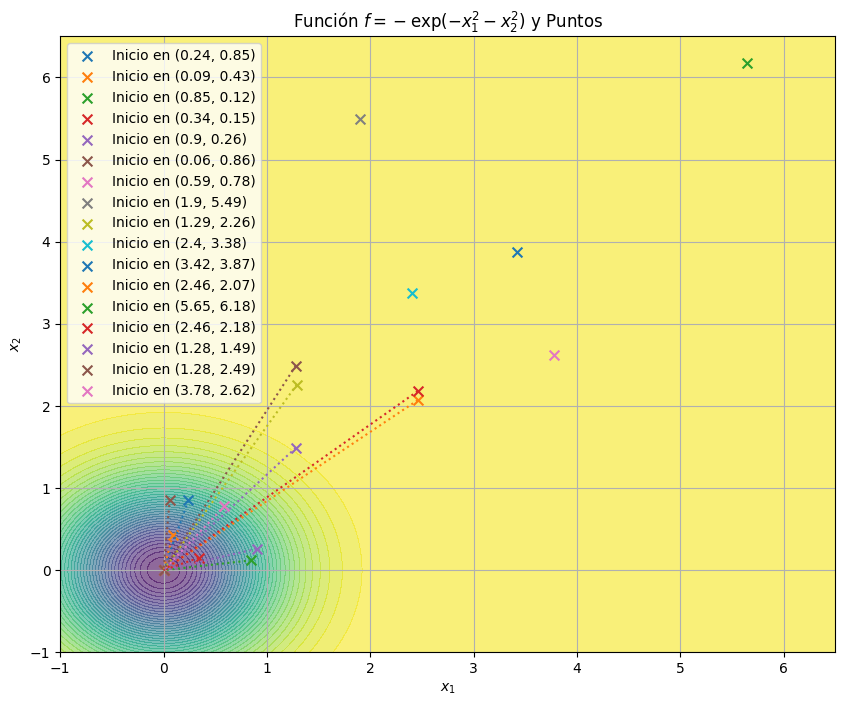
\includegraphics[width=0.65\linewidth]{figuras/PREG7_UNI.png}
    \label{fig:enter-label}
\end{figure}

\item Utilizando busqueda de Armijo


\begin{table}[H]
\centering
\renewcommand{\arraystretch}{1.2}
\begin{tabular}{|c|c|c|c|c|c|c|}
\hline
\textbf{It$_{total}$} & \textbf{Arm$_{total}$} &\textbf{x$_{inicial}$} & \textbf{$\mathbf{x^k}$} & \textbf{|| $\nabla$f($\mathbf{x^k}$) ||} & \textbf{f($\mathbf{x^k}$)}& \textbf{tiempo} \\
\hline
7  & 37 & (0.24 , 0.85) &( 0.00000,0.00000 ) & 0.00000024 & -1.00000000 & 0.1608 \\
7  & 40 & (0.09 , 0.43) &( 0.00000,0.00000 ) & 0.00000076 & -1.00000000 & 0.1892 \\
10  & 39 & (0.85 , 0.12) &( 0.00000,0.00000 ) & 0.00000024 & -1.00000000 & 0.1975 \\
9  & 40 & (0.34 , 0.15) &( 0.00000,0.00000 ) & 0.00000073 & -1.00000000 & 0.2099 \\
8  & 40 & (0.9 , 0.26) &( 0.00000,0.00000 ) & 0.00000026 & -1.00000000 & 0.1669 \\
10  & 40 & (0.06 , 0.86) &( 0.00000,0.00000 ) & 0.00000008 & -1.00000000 & 0.1989 \\
10  & 42 & (0.59 , 0.78) &( 0.00000,0.00000 ) & 0.00000042 & -1.00000000 & 0.1721 \\
1  & 0 & (1.9 , 5.49) &( 1.90000,5.49000 ) & 0.00000000 & -0.00000000 & 0.0000 \\
43  & 74 & (1.29 , 2.26) &( -0.00000,-0.00000 ) & 0.00000024 & -1.00000000 & 0.4141 \\
1  & 0 & (2.4 , 3.38) &( 2.40000,3.38000 ) & 0.00000029 & -0.00000003 & 0.0000 \\
1  & 0 & (3.42 , 3.87) &( 3.42000,3.87000 ) & 0.00000000 & -0.00000000 & 0.0000 \\
685  & 711 & (2.46 , 2.07) &( 0.00000,0.00000 ) & 0.00000058 & -1.00000000 & 5.5139 \\
1  & 0 & (5.65 , 6.18) &( 5.65000,6.18000 ) & 0.00000000 & -0.00000000 & 0.0000 \\
1033  & 1064 & (2.46 , 2.18) &( 0.00000,0.00000 ) & 0.00000007 & -1.00000000 & 7.3213 \\
15  & 61 & (1.28 , 1.49) &( 0.00000,0.00000 ) & 0.00000080 & -1.00000000 & 0.2207 \\
89  & 127 & (1.28 , 2.49) &( 0.00000,0.00000 ) & 0.00000066 & -1.00000000 & 0.7162 \\
1  & 0 & (3.78 , 2.62) &( 3.78000,2.62000 ) & 0.00000001 & -0.00000000 & 0.0000 \\
\hline
\end{tabular}
\end{table}

\begin{figure}
    \centering
    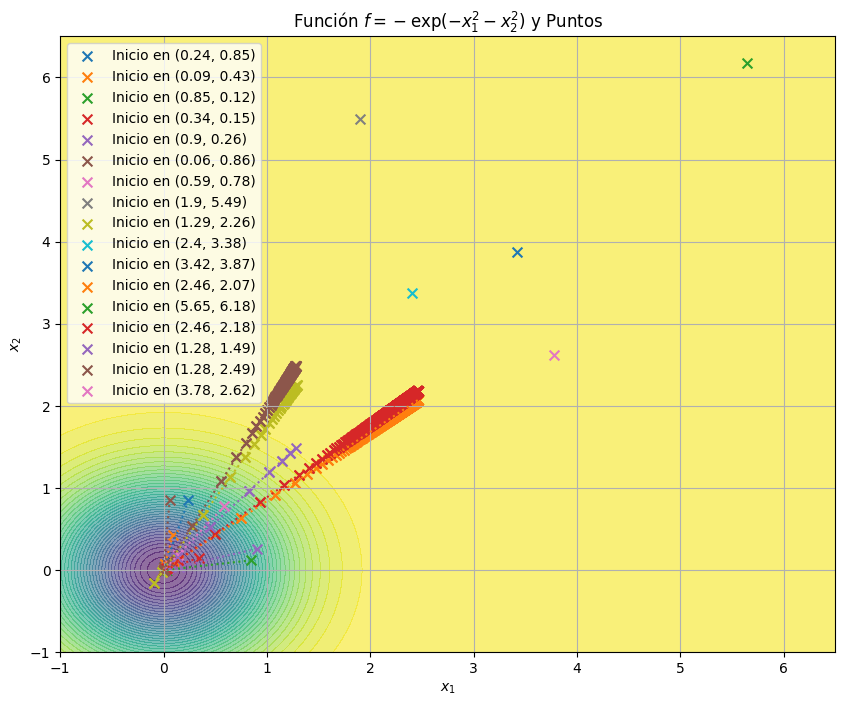
\includegraphics[width=0.65\linewidth]{figuras/PREG7_ARMIJO.png}
    \label{fig:enter-label}
\end{figure}

\end{itemize}

    
    \item Resultados de aplicar el método del punto proximal.
    \begin{itemize}
\item  Utilizando $\lambda_k = \frac{1}{15}$

\begin{table}[H]
\centering
\renewcommand{\arraystretch}{1.2} 
\begin{tabular}{|c|c|c|c|c|c|}
\hline
\textbf{Iter} & \textbf{x$_{inicial}$} & \textbf{$x^k$} & \textbf{||$\nabla \mathbf{f(x^k)}$}|| & \textbf{f($\mathbf{x^k}$)} & \textbf{tiempo} \\
\hline
16   & (0.2400 , 0.8500) & (0.00000, 0.00000) & 0.00000096 & -1.00000000 & 0.4619 \\
16   & (0.0900 , 0.4300) & (0.00000, 0.00000) & 0.00000096 & -1.00000000 & 0.4217 \\
16   & (0.8500 , 0.1200) & (0.00000, 0.00000) & 0.00000096 & -1.00000000 & 0.3320 \\
16   & (0.3400 , 0.1500) & (0.00000, 0.00000) & 0.00000092 & -1.00000000 & 0.3299 \\
17   & (0.9000 , 0.2600) & (0.00000, 0.00000) & 0.00000089 & -1.00000000 & 0.3590 \\
16   & (0.0600 , 0.8600) & (0.00000, 0.00000) & 0.00000096 & -1.00000000 & 0.3548 \\
17   & (0.5900 , 0.7800) & (0.00000, 0.00000) & 0.00000087 & -1.00000000 & 0.3452 \\
1   & (1.9000 , 5.4900) & (1.90000, 5.49000) & 0.00000000 & -0.00000000 & 0.0000 \\
54   & (1.2900 , 2.2600) & (0.00000, 0.00000) & 0.00000094 & -1.00000000 & 1.8309 \\
1   & (2.4000 , 3.3800) & (2.40000, 3.38000) & 0.00000029 & -0.00000003 & 0.0000 \\
1   & (3.4200 , 3.8700) & (3.42000, 3.87000) & 0.00000000 & -0.00000000 & 0.0000 \\
854   & (2.4600 , 2.0700) & (0.00000, 0.00000) & 0.00000090 & -1.00000000 & 37.8122 \\
1   & (5.6500 , 6.1800) & (5.65000, 6.18000) & 0.00000000 & -0.00000000 & 0.0000 \\
1289   & (2.4600 , 2.1800) & (0.00000, 0.00000) & 0.00000096 & -1.00000000 & 53.7023 \\
19   & (1.2800 , 1.4900) & (0.00000, 0.00000) & 0.00000096 & -1.00000000 & 0.5334 \\
109   & (1.2800 , 2.4900) & (0.00000, 0.00000) & 0.00000094 & -1.00000000 & 4.2652 \\
1   & (3.7800 , 2.6200) & (3.78000, 2.62000) & 0.00000001 & -0.00000000 & 0.0000 \\
\hline
\end{tabular}
\end{table}

\begin{figure}
    \centering
    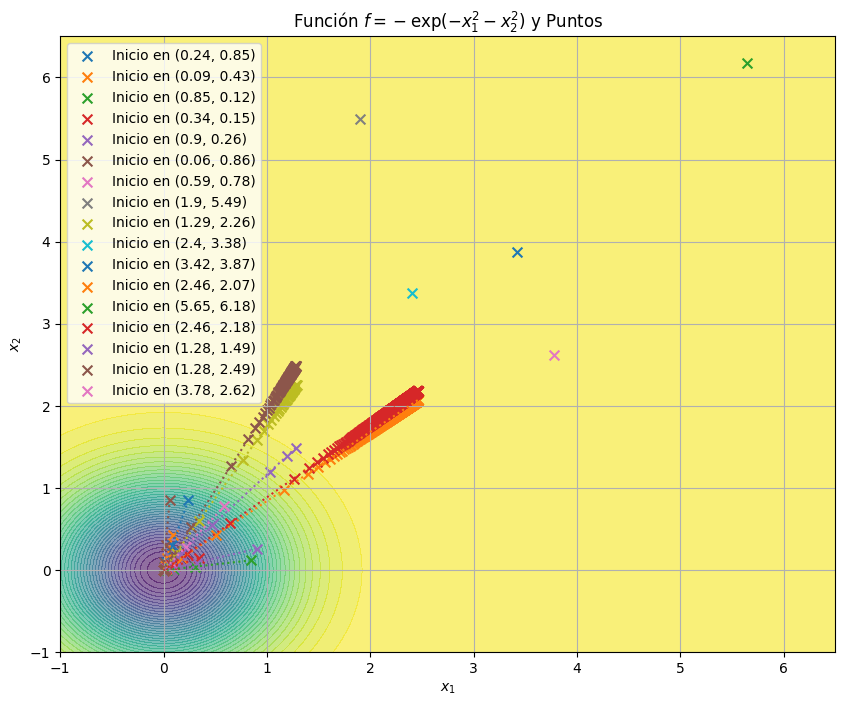
\includegraphics[width=0.65\linewidth]{figuras/PREG8_GRAD.png}   
    \label{fig:enter-label}
\end{figure}


\item Utilizando el método de descenso de gradiente con busqueda de Armijo

\begin{table}[H]
\centering
\renewcommand{\arraystretch}{1.2} 
\begin{tabular}{|c|c|c|c|c|c|c|c|}
\hline
\textbf{Iter$_{total}$} &\textbf{Des$_{total}$}&\textbf{Arm$_{total}$} & \textbf{x$_{inicial}$}& \textbf{$x^k$} & \textbf{||$\nabla \mathbf{f(x^k)}$}|| & \textbf{f($\mathbf{x^k}$)} & \textbf{tiempo} \\
\hline
15  & 88 &260 & (0.24 , 0.85) &( 0.00000,0.00000 ) & 0.00000079 & -1.00000000 & 4.7337 \\
15  & 77 &228 & (0.09 , 0.43) &( 0.00000,0.00000 ) & 0.00000055 & -1.00000000 & 4.7221 \\
15  & 88 &260 & (0.85 , 0.12) &( 0.00000,0.00000 ) & 0.00000076 & -1.00000000 & 5.8824 \\
14  & 75 &222 & (0.34 , 0.15) &( 0.00000,0.00000 ) & 0.00000093 & -1.00000000 & 4.0884 \\
15  & 82 &241 & (0.9 , 0.26) &( 0.00000,0.00000 ) & 0.00000084 & -1.00000000 & 5.1413 \\
15  & 88 &260 & (0.06 , 0.86) &( 0.00000,0.00000 ) & 0.00000077 & -1.00000000 & 4.2686 \\
15  & 90 &265 & (0.59 , 0.78) &( 0.00000,0.00000 ) & 0.00000089 & -1.00000000 & 4.9996 \\
1  & 1 &0 & (1.9 , 5.49) &( 1.90000,5.49000 ) & 0.00000000 & -0.00000000 & 0.0000 \\
52  & 283 &453 & (1.29 , 2.26) &( 0.00000,0.00000 ) & 0.00000080 & -1.00000000 & 18.3300 \\
1  & 1 &0 & (2.4 , 3.38) &( 2.40000,3.38000 ) & 0.00000029 & -0.00000003 & 0.0000 \\
1  & 1 &0 & (3.42 , 3.87) &( 3.42000,3.87000 ) & 0.00000000 & -0.00000000 & 0.0000 \\
851  & 1537 &1702 & (2.46 , 2.07) &( 0.00000,0.00000 ) & 0.00000065 & -1.00000000 & 180.5773 \\
1  & 1 &0 & (5.65 , 6.18) &( 5.65000,6.18000 ) & 0.00000000 & -0.00000000 & 0.0000 \\
1285  & 1942 &2111 & (2.46 , 2.18) &( 0.00000,0.00000 ) & 0.00000081 & -1.00000000 & 251.5819 \\
18  & 129 &287 & (1.28 , 1.49) &( 0.00000,0.00000 ) & 0.00000084 & -1.00000000 & 5.9728 \\
108  & 436 &598 & (1.28 , 2.49) &( 0.00000,0.00000 ) & 0.00000068 & -1.00000000 & 29.0050 \\
1  & 1 &0 & (3.78 , 2.62) &( 3.78000,2.62000 ) & 0.00000001 & -0.00000000 & 0.0000 \\
\hline
\end{tabular}
\end{table}

\begin{figure}
    \centering
    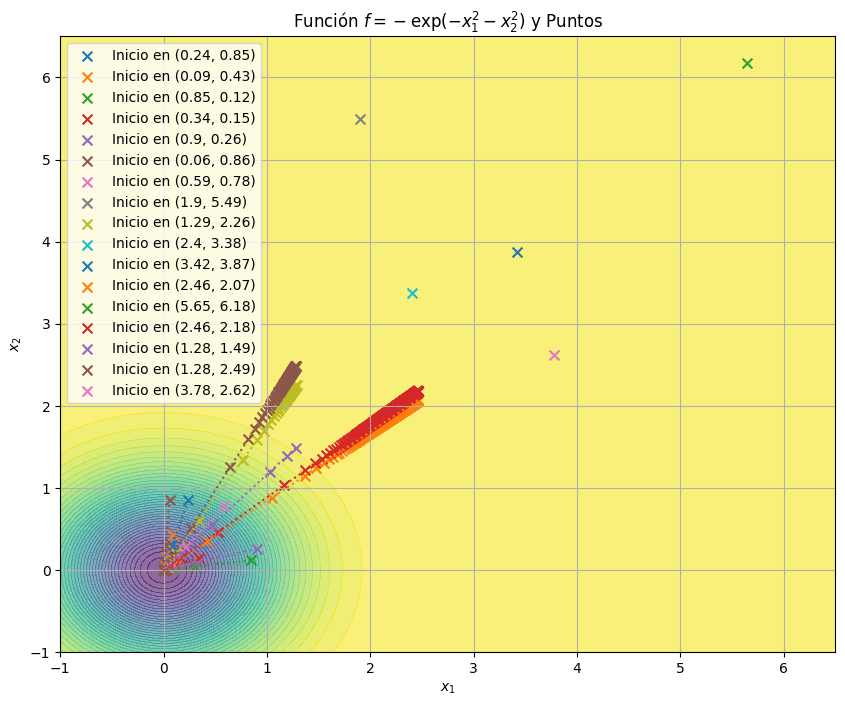
\includegraphics[width=0.65\linewidth]{figuras/PREG8_ARMIJO.png}
    \label{fig:enter-label}
\end{figure}

\begin{itemize}
    \item \textbf{Observaciones del algoritmo :}\\
    En este algoritmo el arreglo de hacer un cambio de la forma \[ x_{k+1} = \quad  arg min \quad \{ f(X)+(1/2) *||X-x^k||^2 \} \] hace posible probar con un punto más lejano a $(0,0)$, para poder encontrar el mínimo $(0,0)$
\end{itemize}
\end{itemize}




    
    \item Conclusiones
    \begin{itemize}
    \item Los métodos y puntos probados con búsqueda de Armijo necesitan más tiempo de ejecución    
    \item Se obtiene menores cantidad de iteracioens con busqueda exacta, pero a la ves puede ser de alto costo computacional el resolver la ecuación que plantee este algoritmo:
\[\lambda_k \in  argmin\{ f(x^k-\lambda \nabla f(x^k) ) \}\]
así como tambien el hecho de no encontrar raices reales como resultado de resolver dicha ecuación, lo que haría que se detenga el algoritmo.

\end{itemize}

    %\item Código implementado para el trabajo
    %\begin{itemize}
\item  Previos 
 
    \begin{tcolorbox}[breakable, size=fbox, boxrule=1pt, pad at break*=1mm,colback=cellbackground, colframe=cellborder]
\prompt{In}{incolor}{ }{\boxspacing}
\begin{Verbatim}[commandchars=\\\{\}]
\PY{c+c1}{\PYZsh{} COLECCION DE PUNTOS Y LIBRERIAS}
\PY{k+kn}{import} \PY{n+nn}{numpy} \PY{k}{as} \PY{n+nn}{np}
\PY{k+kn}{import} \PY{n+nn}{matplotlib}\PY{n+nn}{.}\PY{n+nn}{pyplot} \PY{k}{as} \PY{n+nn}{plt}
\PY{k+kn}{import} \PY{n+nn}{time}
\PY{k+kn}{import} \PY{n+nn}{sympy} \PY{k}{as} \PY{n+nn}{sp}
\PY{n}{x1}\PY{p}{,} \PY{n}{x2}\PY{p}{,}\PY{n}{l}\PY{o}{=} \PY{n}{sp}\PY{o}{.}\PY{n}{symbols}\PY{p}{(}\PY{l+s+s1}{\PYZsq{}}\PY{l+s+s1}{x1 x2 l}\PY{l+s+s1}{\PYZsq{}}\PY{p}{)}
\PY{n}{nuevos} \PY{o}{=} \PY{n}{np}\PY{o}{.}\PY{n}{array}\PY{p}{(}\PY{p}{[}
    \PY{p}{[}\PY{l+m+mf}{0.24}\PY{p}{,} \PY{l+m+mf}{0.85}\PY{p}{]}\PY{p}{,}
    \PY{p}{[}\PY{l+m+mf}{0.09}\PY{p}{,} \PY{l+m+mf}{0.43}\PY{p}{]}\PY{p}{,}
    \PY{p}{[}\PY{l+m+mf}{0.85}\PY{p}{,} \PY{l+m+mf}{0.12}\PY{p}{]}\PY{p}{,}
    \PY{p}{[}\PY{l+m+mf}{0.34}\PY{p}{,} \PY{l+m+mf}{0.15}\PY{p}{]}\PY{p}{,}
    \PY{p}{[}\PY{l+m+mf}{0.9}\PY{p}{,} \PY{l+m+mf}{0.26}\PY{p}{]}\PY{p}{,}
    \PY{p}{[}\PY{l+m+mf}{0.06}\PY{p}{,} \PY{l+m+mf}{0.86}\PY{p}{]}\PY{p}{,}
    \PY{p}{[}\PY{l+m+mf}{0.59}\PY{p}{,} \PY{l+m+mf}{0.78}\PY{p}{]}\PY{p}{,}
    \PY{p}{[}\PY{l+m+mf}{1.9}\PY{p}{,} \PY{l+m+mf}{5.49}\PY{p}{]}\PY{p}{,}
    \PY{p}{[}\PY{l+m+mf}{1.29}\PY{p}{,}\PY{l+m+mf}{2.26}\PY{p}{]}\PY{p}{,}
    \PY{p}{[}\PY{l+m+mf}{2.4}\PY{p}{,} \PY{l+m+mf}{3.38}\PY{p}{]}\PY{p}{,}
    \PY{p}{[}\PY{l+m+mf}{3.42}\PY{p}{,} \PY{l+m+mf}{3.87}\PY{p}{]}\PY{p}{,}
    \PY{p}{[}\PY{l+m+mf}{2.46}\PY{p}{,} \PY{l+m+mf}{2.07}\PY{p}{]}\PY{p}{,}
    \PY{p}{[}\PY{l+m+mf}{5.65}\PY{p}{,} \PY{l+m+mf}{6.18}\PY{p}{]}\PY{p}{,}
    \PY{p}{[}\PY{l+m+mf}{2.46}\PY{p}{,} \PY{l+m+mf}{2.18}\PY{p}{]}\PY{p}{,}
    \PY{p}{[}\PY{l+m+mf}{1.28}\PY{p}{,} \PY{l+m+mf}{1.49}\PY{p}{]}\PY{p}{,}
    \PY{p}{[}\PY{l+m+mf}{1.28}\PY{p}{,} \PY{l+m+mf}{2.49}\PY{p}{]}\PY{p}{,}
    \PY{p}{[}\PY{l+m+mf}{3.78}\PY{p}{,} \PY{l+m+mf}{2.62}\PY{p}{]} 
\PY{p}{]}\PY{p}{)}
\end{Verbatim}
\end{tcolorbox}

\item Gráfico de puntos y superficie.
    \begin{tcolorbox}[breakable, size=fbox, boxrule=1pt, pad at break*=1mm,colback=cellbackground, colframe=cellborder]
\prompt{In}{incolor}{ }{\boxspacing}
\begin{Verbatim}[commandchars=\\\{\}]
\PY{c+c1}{\PYZsh{} GRAFICO DE PUNTOS Y SUPERFICIE}
\PY{k}{def} \PY{n+nf}{graficoPuntos}\PY{p}{(}\PY{n}{puntos}\PY{p}{,}\PY{n}{dx}\PY{o}{=}\PY{l+m+mi}{5}\PY{p}{,}\PY{n}{dy}\PY{o}{=}\PY{l+m+mi}{5}\PY{p}{)}\PY{p}{:}
    \PY{k}{def} \PY{n+nf}{f}\PY{p}{(}\PY{n}{x1}\PY{p}{,} \PY{n}{x2}\PY{p}{)}\PY{p}{:}
        \PY{k}{return} \PY{o}{\PYZhy{}}\PY{n}{np}\PY{o}{.}\PY{n}{exp}\PY{p}{(}\PY{o}{\PYZhy{}}\PY{n}{x1}\PY{o}{*}\PY{o}{*}\PY{l+m+mi}{2} \PY{o}{\PYZhy{}} \PY{n}{x2}\PY{o}{*}\PY{o}{*}\PY{l+m+mi}{2}\PY{p}{)}
    \PY{n}{x1} \PY{o}{=} \PY{n}{np}\PY{o}{.}\PY{n}{linspace}\PY{p}{(}\PY{o}{\PYZhy{}}\PY{l+m+mi}{1}\PY{p}{,} \PY{n}{dx}\PY{p}{,} \PY{l+m+mi}{200}\PY{p}{)}
    \PY{n}{x2} \PY{o}{=} \PY{n}{np}\PY{o}{.}\PY{n}{linspace}\PY{p}{(}\PY{o}{\PYZhy{}}\PY{l+m+mi}{1}\PY{p}{,} \PY{n}{dy}\PY{p}{,} \PY{l+m+mi}{200}\PY{p}{)}
    \PY{n}{x1}\PY{p}{,} \PY{n}{x2} \PY{o}{=} \PY{n}{np}\PY{o}{.}\PY{n}{meshgrid}\PY{p}{(}\PY{n}{x1}\PY{p}{,} \PY{n}{x2}\PY{p}{)}
    \PY{n}{z} \PY{o}{=} \PY{n}{f}\PY{p}{(}\PY{n}{x1}\PY{p}{,} \PY{n}{x2}\PY{p}{)}
    \PY{n}{plt}\PY{o}{.}\PY{n}{figure}\PY{p}{(}\PY{n}{figsize}\PY{o}{=}\PY{p}{(}\PY{l+m+mi}{10}\PY{p}{,} \PY{l+m+mi}{8}\PY{p}{)}\PY{p}{)}
    \PY{n}{plt}\PY{o}{.}\PY{n}{contourf}\PY{p}{(}\PY{n}{x1}\PY{p}{,} \PY{n}{x2}\PY{p}{,} \PY{n}{z}\PY{p}{,} \PY{n}{levels}\PY{o}{=}\PY{l+m+mi}{40}\PY{p}{,} \PY{n}{cmap}\PY{o}{=}\PY{l+s+s1}{\PYZsq{}}\PY{l+s+s1}{viridis}\PY{l+s+s1}{\PYZsq{}}\PY{p}{,}\PY{n}{alpha}\PY{o}{=}\PY{l+m+mf}{0.6}\PY{p}{)}
    \PY{k}{for} \PY{n}{i}\PY{p}{,} \PY{n}{puntos\PYZus{}trayectoria} \PY{o+ow}{in} \PY{n+nb}{enumerate}\PY{p}{(}\PY{n}{puntos}\PY{p}{)}\PY{p}{:}
        \PY{k}{if} \PY{n+nb}{len}\PY{p}{(}\PY{n}{puntos\PYZus{}trayectoria}\PY{p}{)} \PY{o}{\PYZlt{}} \PY{l+m+mi}{1}\PY{p}{:}
            \PY{n+nb}{print}\PY{p}{(}\PY{l+s+sa}{f}\PY{l+s+s2}{\PYZdq{}}\PY{l+s+s2}{La trayectoria }\PY{l+s+si}{\PYZob{}}\PY{n}{i}\PY{o}{+}\PY{l+m+mi}{1}\PY{l+s+si}{\PYZcb{}}\PY{l+s+s2}{ está vacía.}\PY{l+s+s2}{\PYZdq{}}\PY{p}{)}
            \PY{k}{continue}
        \PY{n}{x\PYZus{}inicio} \PY{o}{=} \PY{n}{puntos\PYZus{}trayectoria}\PY{p}{[}\PY{l+m+mi}{0}\PY{p}{]}\PY{p}{[}\PY{l+m+mi}{0}\PY{p}{]}
        \PY{n}{y\PYZus{}inicio} \PY{o}{=} \PY{n}{puntos\PYZus{}trayectoria}\PY{p}{[}\PY{l+m+mi}{0}\PY{p}{]}\PY{p}{[}\PY{l+m+mi}{1}\PY{p}{]}
        \PY{n}{x\PYZus{}values} \PY{o}{=} \PY{p}{[}\PY{n}{point}\PY{p}{[}\PY{l+m+mi}{0}\PY{p}{]} \PY{k}{for} \PY{n}{point} \PY{o+ow}{in} \PY{n}{puntos\PYZus{}trayectoria}\PY{p}{]}
        \PY{n}{y\PYZus{}values} \PY{o}{=} \PY{p}{[}\PY{n}{point}\PY{p}{[}\PY{l+m+mi}{1}\PY{p}{]} \PY{k}{for} \PY{n}{point} \PY{o+ow}{in} \PY{n}{puntos\PYZus{}trayectoria}\PY{p}{]}
        \PY{n}{plt}\PY{o}{.}\PY{n}{scatter}\PY{p}{(}\PY{n}{x\PYZus{}values}\PY{p}{,} \PY{n}{y\PYZus{}values}\PY{p}{,} \PY{n}{marker}\PY{o}{=}\PY{l+s+s1}{\PYZsq{}}\PY{l+s+s1}{x}\PY{l+s+s1}{\PYZsq{}}\PY{p}{,} \PY{n}{s}\PY{o}{=}\PY{l+m+mi}{50}\PY{p}{,} \PY{n}{label}\PY{o}{=}\PY{l+s+sa}{f}\PY{l+s+s1}{\PYZsq{}}\PY{l+s+s1}{Inicio en (}\PY{l+s+si}{\PYZob{}}\PY{n}{x\PYZus{}inicio}\PY{l+s+si}{\PYZcb{}}\PY{l+s+s1}{, }\PY{l+s+si}{\PYZob{}}\PY{n}{y\PYZus{}inicio}\PY{l+s+si}{\PYZcb{}}\PY{l+s+s1}{)}\PY{l+s+s1}{\PYZsq{}}\PY{p}{)}
        \PY{n}{plt}\PY{o}{.}\PY{n}{plot}\PY{p}{(}\PY{n}{x\PYZus{}values}\PY{p}{,} \PY{n}{y\PYZus{}values}\PY{p}{,} \PY{n}{linestyle}\PY{o}{=}\PY{l+s+s1}{\PYZsq{}}\PY{l+s+s1}{dotted}\PY{l+s+s1}{\PYZsq{}}\PY{p}{)}
    \PY{n}{plt}\PY{o}{.}\PY{n}{title}\PY{p}{(}\PY{l+s+sa}{r}\PY{l+s+s1}{\PYZsq{}}\PY{l+s+s1}{Función \PYZdl{}f = \PYZhy{}}\PY{l+s+s1}{\PYZbs{}}\PY{l+s+s1}{exp(\PYZhy{}x\PYZus{}1\PYZca{}2 \PYZhy{} x\PYZus{}2\PYZca{}2)\PYZdl{} y Puntos}\PY{l+s+s1}{\PYZsq{}}\PY{p}{)}
    \PY{n}{plt}\PY{o}{.}\PY{n}{xlabel}\PY{p}{(}\PY{l+s+sa}{r}\PY{l+s+s1}{\PYZsq{}}\PY{l+s+s1}{\PYZdl{}x\PYZus{}1\PYZdl{}}\PY{l+s+s1}{\PYZsq{}}\PY{p}{)}
    \PY{n}{plt}\PY{o}{.}\PY{n}{ylabel}\PY{p}{(}\PY{l+s+sa}{r}\PY{l+s+s1}{\PYZsq{}}\PY{l+s+s1}{\PYZdl{}x\PYZus{}2\PYZdl{}}\PY{l+s+s1}{\PYZsq{}}\PY{p}{)}
    \PY{n}{plt}\PY{o}{.}\PY{n}{legend}\PY{p}{(}\PY{n}{loc}\PY{o}{=}\PY{l+s+s1}{\PYZsq{}}\PY{l+s+s1}{upper left}\PY{l+s+s1}{\PYZsq{}}\PY{p}{)}
    \PY{n}{plt}\PY{o}{.}\PY{n}{grid}\PY{p}{(}\PY{k+kc}{True}\PY{p}{)}
    \PY{n}{plt}\PY{o}{.}\PY{n}{show}\PY{p}{(}\PY{p}{)}
\end{Verbatim}
\end{tcolorbox}

\item Fucinones de búsqueda de Armijo y búsqueda exacta:

    \begin{tcolorbox}[breakable, size=fbox, boxrule=1pt, pad at break*=1mm,colback=cellbackground, colframe=cellborder]
\prompt{In}{incolor}{ }{\boxspacing}
\begin{Verbatim}[commandchars=\\\{\}]
\PY{k}{def} \PY{n+nf}{b\PYZus{}unidimensional}\PY{p}{(}\PY{n}{u}\PY{p}{,}\PY{n}{gU}\PY{p}{)}\PY{p}{:}
    \PY{n}{gU} \PY{o}{=} \PY{n}{sp}\PY{o}{.}\PY{n}{sympify}\PY{p}{(}\PY{n}{gU}\PY{p}{)}
    \PY{n}{ec} \PY{o}{=} \PY{n}{gU}\PY{o}{.}\PY{n}{subs}\PY{p}{(}\PY{p}{\PYZob{}}\PY{n}{x1}\PY{p}{:} \PY{n}{u}\PY{p}{[}\PY{l+m+mi}{0}\PY{p}{]}\PY{p}{,} \PY{n}{x2}\PY{p}{:} \PY{n}{u}\PY{p}{[}\PY{l+m+mi}{1}\PY{p}{]}\PY{p}{\PYZcb{}}\PY{p}{)}
    \PY{n}{derivada\PYZus{}ec} \PY{o}{=} \PY{n}{sp}\PY{o}{.}\PY{n}{diff}\PY{p}{(}\PY{n}{ec}\PY{p}{,} \PY{n}{l}\PY{p}{)}
    \PY{n}{sol} \PY{o}{=} \PY{n}{sp}\PY{o}{.}\PY{n}{solve}\PY{p}{(}\PY{n}{derivada\PYZus{}ec}\PY{p}{,} \PY{n}{l}\PY{p}{)}
    \PY{n}{sol\PYZus{}reales} \PY{o}{=} \PY{p}{[}\PY{n}{s}\PY{o}{.}\PY{n}{evalf}\PY{p}{(}\PY{p}{)} \PY{k}{for} \PY{n}{s} \PY{o+ow}{in} \PY{n}{sol} \PY{k}{if} \PY{n}{sp}\PY{o}{.}\PY{n}{im}\PY{p}{(}\PY{n}{s}\PY{p}{)} \PY{o}{==} \PY{l+m+mi}{0}\PY{p}{]}
    \PY{k}{if} \PY{o+ow}{not} \PY{n}{sol\PYZus{}reales}\PY{p}{:}
        \PY{k}{return} \PY{l+s+s1}{\PYZsq{}}\PY{l+s+s1}{N}\PY{l+s+s1}{\PYZsq{}}
    \PY{k}{else}\PY{p}{:}
        \PY{n}{min\PYZus{}valores} \PY{o}{=} \PY{p}{[}\PY{n}{ec}\PY{o}{.}\PY{n}{subs}\PY{p}{(}\PY{p}{\PYZob{}}\PY{n}{l}\PY{p}{:} \PY{n}{i}\PY{p}{\PYZcb{}}\PY{p}{)}\PY{o}{.}\PY{n}{evalf}\PY{p}{(}\PY{p}{)} \PY{k}{for} \PY{n}{i} \PY{o+ow}{in} \PY{n}{sol\PYZus{}reales}\PY{p}{]}
        \PY{n}{l\PYZus{}min\PYZus{}} \PY{o}{=} \PY{n}{sol\PYZus{}reales}\PY{p}{[}\PY{n}{min\PYZus{}valores}\PY{o}{.}\PY{n}{index}\PY{p}{(}\PY{n+nb}{min}\PY{p}{(}\PY{n}{min\PYZus{}valores}\PY{p}{)}\PY{p}{)}\PY{p}{]}
    \PY{k}{return} \PY{n}{l\PYZus{}min\PYZus{}}

\PY{k}{def} \PY{n+nf}{b\PYZus{}armijo}\PY{p}{(}\PY{n}{fA}\PY{p}{,} \PY{n}{x0\PYZus{}}\PY{p}{,} \PY{n}{d}\PY{o}{=}\PY{k+kc}{None}\PY{p}{)}\PY{p}{:}
    \PY{n}{fA} \PY{o}{=} \PY{n}{sp}\PY{o}{.}\PY{n}{sympify}\PY{p}{(}\PY{n}{fA}\PY{p}{)}
    \PY{n}{s} \PY{o}{=} \PY{l+m+mi}{1}
    \PY{n}{beta} \PY{o}{=} \PY{l+m+mf}{0.5}
    \PY{n}{sigma} \PY{o}{=} \PY{l+m+mf}{0.5}
    \PY{n}{m} \PY{o}{=} \PY{l+m+mi}{0}
    \PY{n}{x0\PYZus{}} \PY{o}{=} \PY{n}{np}\PY{o}{.}\PY{n}{array}\PY{p}{(}\PY{n}{x0\PYZus{}}\PY{p}{)}
    \PY{n}{grad} \PY{o}{=} \PY{p}{[}\PY{n}{sp}\PY{o}{.}\PY{n}{diff}\PY{p}{(}\PY{n}{fA}\PY{p}{,} \PY{n}{var}\PY{p}{)} \PY{k}{for} \PY{n}{var} \PY{o+ow}{in} \PY{p}{(}\PY{n}{x1}\PY{p}{,} \PY{n}{x2}\PY{p}{)}\PY{p}{]}
    \PY{n}{grad\PYZus{}func} \PY{o}{=} \PY{n}{sp}\PY{o}{.}\PY{n}{lambdify}\PY{p}{(}\PY{p}{(}\PY{n}{x1}\PY{p}{,} \PY{n}{x2}\PY{p}{)}\PY{p}{,} \PY{n}{grad}\PY{p}{)}
    \PY{n}{grad\PYZus{}eval} \PY{o}{=} \PY{n}{grad\PYZus{}func}\PY{p}{(}\PY{o}{*}\PY{n}{x0\PYZus{}}\PY{p}{)}
    \PY{k}{if} \PY{n}{d} \PY{o+ow}{is} \PY{k+kc}{None}\PY{p}{:}
        \PY{n}{d} \PY{o}{=} \PY{o}{\PYZhy{}}\PY{l+m+mi}{1} \PY{o}{*} \PY{n}{np}\PY{o}{.}\PY{n}{array}\PY{p}{(}\PY{n}{grad\PYZus{}eval}\PY{p}{)}
    \PY{n}{res1} \PY{o}{=} \PY{n+nb}{float}\PY{p}{(}\PY{n}{fA}\PY{o}{.}\PY{n}{subs}\PY{p}{(}\PY{p}{\PYZob{}}\PY{n}{x1}\PY{p}{:} \PY{n}{x0\PYZus{}}\PY{p}{[}\PY{l+m+mi}{0}\PY{p}{]}\PY{p}{,} \PY{n}{x2}\PY{p}{:} \PY{n}{x0\PYZus{}}\PY{p}{[}\PY{l+m+mi}{1}\PY{p}{]}\PY{p}{\PYZcb{}}\PY{p}{)}\PY{p}{)}
    \PY{n}{mod} \PY{o}{=} \PY{n}{np}\PY{o}{.}\PY{n}{dot}\PY{p}{(}\PY{n}{np}\PY{o}{.}\PY{n}{array}\PY{p}{(}\PY{n}{grad\PYZus{}eval}\PY{p}{)}\PY{o}{.}\PY{n}{T}\PY{p}{,} \PY{n}{d}\PY{p}{)}
    \PY{k}{while} \PY{k+kc}{True}\PY{p}{:}
        \PY{n}{eval\PYZus{}} \PY{o}{=} \PY{p}{\PYZob{}}\PY{n}{x1}\PY{p}{:} \PY{n}{x0\PYZus{}}\PY{p}{[}\PY{l+m+mi}{0}\PY{p}{]} \PY{o}{+} \PY{p}{(}\PY{n}{s} \PY{o}{*} \PY{n}{beta} \PY{o}{*}\PY{o}{*} \PY{n}{m}\PY{p}{)} \PY{o}{*} \PY{n}{d}\PY{p}{[}\PY{l+m+mi}{0}\PY{p}{]}\PY{p}{,} \PY{n}{x2}\PY{p}{:} \PY{n}{x0\PYZus{}}\PY{p}{[}\PY{l+m+mi}{1}\PY{p}{]} \PY{o}{+} \PY{p}{(}\PY{n}{s} \PY{o}{*} \PY{n}{beta} \PY{o}{*}\PY{o}{*} \PY{n}{m}\PY{p}{)} \PY{o}{*} \PY{n}{d}\PY{p}{[}\PY{l+m+mi}{1}\PY{p}{]}\PY{p}{\PYZcb{}}
        \PY{n}{res2} \PY{o}{=} \PY{n+nb}{float}\PY{p}{(}\PY{n}{fA}\PY{o}{.}\PY{n}{subs}\PY{p}{(}\PY{n}{eval\PYZus{}}\PY{p}{)}\PY{p}{)}
        \PY{n}{res3} \PY{o}{=} \PY{n+nb}{float}\PY{p}{(}\PY{p}{(}\PY{o}{\PYZhy{}}\PY{n}{sigma} \PY{o}{*} \PY{n}{s} \PY{o}{*} \PY{n}{beta} \PY{o}{*}\PY{o}{*} \PY{n}{m}\PY{p}{)} \PY{o}{*} \PY{n}{mod}\PY{p}{)}
        \PY{k}{if} \PY{n}{res1} \PY{o}{\PYZhy{}} \PY{n}{res2} \PY{o}{\PYZgt{}}\PY{o}{=} \PY{n}{res3}\PY{p}{:}
            \PY{k}{return} \PY{n}{s} \PY{o}{*} \PY{p}{(}\PY{n}{beta} \PY{o}{*}\PY{o}{*} \PY{n}{m}\PY{p}{)}\PY{p}{,} \PY{n}{m}
        \PY{k}{else}\PY{p}{:}
            \PY{n}{m} \PY{o}{+}\PY{o}{=} \PY{l+m+mi}{1}
\end{Verbatim}
\end{tcolorbox}

\item Método iterativo de Descenso de gradiente con búsqueda unidimensional
  \begin{tcolorbox}[breakable, size=fbox, boxrule=1pt, pad at break*=1mm,colback=cellbackground, colframe=cellborder]
\prompt{In}{incolor}{ }{\boxspacing}
\begin{Verbatim}[commandchars=\\\{\}]
\PY{c+c1}{\PYZsh{} DESCENSO DE GRADIENTE CON BÚSQUEDA EXACTA}
\PY{n}{eps} \PY{o}{=} \PY{l+m+mf}{1e\PYZhy{}6}
\PY{n}{f}\PY{o}{=}\PY{o}{\PYZhy{}}\PY{n}{sp}\PY{o}{.}\PY{n}{exp}\PY{p}{(}\PY{o}{\PYZhy{}}\PY{n}{x1}\PY{o}{*}\PY{o}{*}\PY{l+m+mi}{2}\PY{o}{\PYZhy{}}\PY{n}{x2}\PY{o}{*}\PY{o}{*}\PY{l+m+mi}{2}\PY{p}{)}
\PY{n}{grad} \PY{o}{=} \PY{p}{[}\PY{n}{sp}\PY{o}{.}\PY{n}{diff}\PY{p}{(}\PY{n}{f}\PY{p}{,} \PY{n}{x1}\PY{p}{)}\PY{p}{,} \PY{n}{sp}\PY{o}{.}\PY{n}{diff}\PY{p}{(}\PY{n}{f}\PY{p}{,} \PY{n}{x2}\PY{p}{)}\PY{p}{]}
\PY{n}{grad\PYZus{}func} \PY{o}{=} \PY{n}{sp}\PY{o}{.}\PY{n}{lambdify}\PY{p}{(}\PY{p}{(}\PY{n}{x1}\PY{p}{,} \PY{n}{x2}\PY{p}{)}\PY{p}{,} \PY{n}{grad}\PY{p}{)}
\PY{n}{todas\PYZus{}las\PYZus{}trayectorias} \PY{o}{=} \PY{p}{[}\PY{p}{]}

\PY{k}{for} \PY{n}{x0} \PY{o+ow}{in} \PY{n}{nuevos}\PY{p}{:}
    \PY{n}{xa}\PY{o}{=}\PY{n}{x0}
    \PY{n}{ext}\PY{o}{=}\PY{l+m+mi}{1}
    \PY{n}{inicio} \PY{o}{=} \PY{n}{time}\PY{o}{.}\PY{n}{time}\PY{p}{(}\PY{p}{)}
    \PY{n}{P}\PY{o}{=}\PY{p}{[}\PY{p}{]}
    \PY{k}{while} \PY{k+kc}{True}\PY{p}{:}
        \PY{n}{P}\PY{o}{.}\PY{n}{append}\PY{p}{(}\PY{n}{x0}\PY{p}{)}
        \PY{n}{grad\PYZus{}eval} \PY{o}{=} \PY{n}{np}\PY{o}{.}\PY{n}{array}\PY{p}{(}\PY{n}{grad\PYZus{}func}\PY{p}{(}\PY{o}{*}\PY{n}{x0}\PY{p}{)}\PY{p}{)}
        \PY{n}{norm\PYZus{}grad} \PY{o}{=} \PY{n}{np}\PY{o}{.}\PY{n}{linalg}\PY{o}{.}\PY{n}{norm}\PY{p}{(}\PY{n}{grad\PYZus{}eval}\PY{p}{)}
        \PY{k}{if}\PY{p}{(}\PY{n}{norm\PYZus{}grad} \PY{o}{\PYZlt{}} \PY{n}{eps}\PY{p}{)}\PY{p}{:}
            \PY{k}{break}
        \PY{n}{g} \PY{o}{=} \PY{n}{x0} \PY{o}{\PYZhy{}} \PY{n}{l} \PY{o}{*} \PY{n}{grad\PYZus{}eval}
        \PY{n}{ec} \PY{o}{=} \PY{n}{f}\PY{o}{.}\PY{n}{subs}\PY{p}{(}\PY{p}{\PYZob{}}\PY{n}{x1}\PY{p}{:} \PY{n}{g}\PY{p}{[}\PY{l+m+mi}{0}\PY{p}{]}\PY{p}{,} \PY{n}{x2}\PY{p}{:} \PY{n}{g}\PY{p}{[}\PY{l+m+mi}{1}\PY{p}{]}\PY{p}{\PYZcb{}}\PY{p}{)}    
        \PY{n}{derivada\PYZus{}ec} \PY{o}{=} \PY{n}{sp}\PY{o}{.}\PY{n}{diff}\PY{p}{(}\PY{n}{ec}\PY{p}{,} \PY{n}{l}\PY{p}{)}
        \PY{n}{sol} \PY{o}{=} \PY{n}{sp}\PY{o}{.}\PY{n}{solve}\PY{p}{(}\PY{n}{derivada\PYZus{}ec}\PY{p}{,} \PY{n}{l}\PY{p}{)}
        \PY{n}{sol\PYZus{}reales} \PY{o}{=} \PY{p}{[}\PY{n}{s}\PY{o}{.}\PY{n}{evalf}\PY{p}{(}\PY{p}{)} \PY{k}{for} \PY{n}{s} \PY{o+ow}{in} \PY{n}{sol} \PY{k}{if} \PY{n}{sp}\PY{o}{.}\PY{n}{im}\PY{p}{(}\PY{n}{s}\PY{p}{)} \PY{o}{==} \PY{l+m+mi}{0}\PY{p}{]}
        \PY{k}{if} \PY{o+ow}{not} \PY{n}{sol\PYZus{}reales}\PY{p}{:}
            \PY{n+nb}{print}\PY{p}{(}\PY{l+s+s2}{\PYZdq{}}\PY{l+s+s2}{No se encontraron soluciones reales.}\PY{l+s+s2}{\PYZdq{}}\PY{p}{)}
            \PY{k}{break}
        \PY{k}{else}\PY{p}{:}
            \PY{n}{min\PYZus{}valores} \PY{o}{=} \PY{p}{[}\PY{n}{ec}\PY{o}{.}\PY{n}{subs}\PY{p}{(}\PY{p}{\PYZob{}}\PY{n}{l}\PY{p}{:} \PY{n}{i}\PY{p}{\PYZcb{}}\PY{p}{)}\PY{o}{.}\PY{n}{evalf}\PY{p}{(}\PY{p}{)} \PY{k}{for} \PY{n}{i} \PY{o+ow}{in} \PY{n}{sol\PYZus{}reales}\PY{p}{]}
            \PY{n}{l\PYZus{}min} \PY{o}{=} \PY{n}{sol\PYZus{}reales}\PY{p}{[}\PY{n}{min\PYZus{}valores}\PY{o}{.}\PY{n}{index}\PY{p}{(}\PY{n+nb}{min}\PY{p}{(}\PY{n}{min\PYZus{}valores}\PY{p}{)}\PY{p}{)}\PY{p}{]}
        \PY{n}{x0} \PY{o}{=} \PY{n}{x0} \PY{o}{\PYZhy{}} \PY{n+nb}{float}\PY{p}{(}\PY{n}{l\PYZus{}min}\PY{p}{)} \PY{o}{*} \PY{n}{grad\PYZus{}eval}
        \PY{n}{ext}\PY{o}{=}\PY{n}{ext}\PY{o}{+}\PY{l+m+mi}{1}
    \PY{n}{grad\PYZus{}eval} \PY{o}{=} \PY{n}{grad\PYZus{}func}\PY{p}{(}\PY{o}{*}\PY{n}{x0}\PY{p}{)}
    \PY{n}{norm\PYZus{}grad} \PY{o}{=} \PY{n}{np}\PY{o}{.}\PY{n}{linalg}\PY{o}{.}\PY{n}{norm}\PY{p}{(}\PY{n}{grad\PYZus{}eval}\PY{p}{)}
    \PY{n}{fin} \PY{o}{=} \PY{n}{time}\PY{o}{.}\PY{n}{time}\PY{p}{(}\PY{p}{)}
    \PY{n}{todas\PYZus{}las\PYZus{}trayectorias}\PY{o}{.}\PY{n}{append}\PY{p}{(}\PY{n}{P}\PY{p}{)}
\PY{c+c1}{\PYZsh{}    print(f\PYZsq{}iter \PYZob{}ext\PYZcb{}  ; armijo \PYZob{}total\PYZus{}armijo\PYZcb{} l\PYZus{}k : \PYZob{}(s*beta**m)\PYZcb{} ; x\PYZus{}inicial \PYZob{}xa\PYZcb{} ; x\PYZus{}encontrado  : \PYZob{}x0[0]:.4f\PYZcb{},\PYZob{}x0[1]:.4f\PYZcb{}; normGrad x0  \PYZob{}norm\PYZus{}grad:.12f\PYZcb{} ; f(x0) \PYZob{}f.subs(\PYZob{}x1:x0[0],x2:x0[1]\PYZcb{}):.12f\PYZcb{}\PYZsq{})}
    \PY{n+nb}{print}\PY{p}{(}\PY{l+s+sa}{f}\PY{l+s+s1}{\PYZsq{}}\PY{l+s+si}{\PYZob{}}\PY{n}{ext}\PY{l+s+si}{\PYZcb{}}\PY{l+s+s1}{  \PYZam{}  (}\PY{l+s+si}{\PYZob{}}\PY{n}{xa}\PY{p}{[}\PY{l+m+mi}{0}\PY{p}{]}\PY{l+s+si}{:}\PY{l+s+s1}{.4}\PY{l+s+si}{\PYZcb{}}\PY{l+s+s1}{ , }\PY{l+s+si}{\PYZob{}}\PY{n}{xa}\PY{p}{[}\PY{l+m+mi}{1}\PY{p}{]}\PY{l+s+si}{:}\PY{l+s+s1}{.4}\PY{l+s+si}{\PYZcb{}}\PY{l+s+s1}{) \PYZam{}( }\PY{l+s+si}{\PYZob{}}\PY{n}{x0}\PY{p}{[}\PY{l+m+mi}{0}\PY{p}{]}\PY{l+s+si}{:}\PY{l+s+s1}{.5f}\PY{l+s+si}{\PYZcb{}}\PY{l+s+s1}{,}\PY{l+s+si}{\PYZob{}}\PY{n}{x0}\PY{p}{[}\PY{l+m+mi}{1}\PY{p}{]}\PY{l+s+si}{:}\PY{l+s+s1}{.5f}\PY{l+s+si}{\PYZcb{}}\PY{l+s+s1}{ ) \PYZam{} }\PY{l+s+si}{\PYZob{}}\PY{n}{norm\PYZus{}grad}\PY{l+s+si}{:}\PY{l+s+s1}{.8f}\PY{l+s+si}{\PYZcb{}}\PY{l+s+s1}{ \PYZam{} }\PY{l+s+si}{\PYZob{}}\PY{n}{f}\PY{o}{.}\PY{n}{subs}\PY{p}{(}\PY{p}{\PYZob{}}\PY{n}{x1}\PY{p}{:}\PY{n}{x0}\PY{p}{[}\PY{l+m+mi}{0}\PY{p}{]}\PY{p}{,}\PY{n}{x2}\PY{p}{:}\PY{n}{x0}\PY{p}{[}\PY{l+m+mi}{1}\PY{p}{]}\PY{p}{\PYZcb{}}\PY{p}{)}\PY{l+s+si}{:}\PY{l+s+s1}{.8f}\PY{l+s+si}{\PYZcb{}}\PY{l+s+s1}{ \PYZam{} }\PY{l+s+si}{\PYZob{}}\PY{p}{(}\PY{n}{fin}\PY{o}{\PYZhy{}}\PY{n}{inicio}\PY{p}{)}\PY{l+s+si}{:}\PY{l+s+s1}{.4f}\PY{l+s+si}{\PYZcb{}}\PY{l+s+s1}{ }\PY{l+s+se}{\PYZbs{}\PYZbs{}}\PY{l+s+se}{\PYZbs{}\PYZbs{}}\PY{l+s+s1}{\PYZsq{}}\PY{p}{)}
\PY{n}{graficoPuntos}\PY{p}{(}\PY{n}{todas\PYZus{}las\PYZus{}trayectorias}\PY{p}{)}
\end{Verbatim}
\end{tcolorbox}


\item Método iterativo de descenso de gradiente con búsqueda de Armijo:


   \begin{tcolorbox}[breakable, size=fbox, boxrule=1pt, pad at break*=1mm,colback=cellbackground, colframe=cellborder]
\prompt{In}{incolor}{ }{\boxspacing}
\begin{Verbatim}[commandchars=\\\{\}]
\PY{c+c1}{\PYZsh{} DESCENSO DE GRADIENTE CON BÚSQUEDA DE ARMIJO}
\PY{n}{f}\PY{o}{=}\PY{o}{\PYZhy{}}\PY{n}{sp}\PY{o}{.}\PY{n}{exp}\PY{p}{(}\PY{o}{\PYZhy{}}\PY{n}{x1}\PY{o}{*}\PY{o}{*}\PY{l+m+mi}{2}\PY{o}{\PYZhy{}}\PY{n}{x2}\PY{o}{*}\PY{o}{*}\PY{l+m+mi}{2}\PY{p}{)}
\PY{n}{s} \PY{o}{=} \PY{l+m+mi}{1}
\PY{n}{beta} \PY{o}{=} \PY{l+m+mi}{1}\PY{o}{/}\PY{l+m+mi}{2}
\PY{n}{sigma} \PY{o}{=} \PY{l+m+mi}{1}\PY{o}{/}\PY{l+m+mi}{2}
\PY{n}{eps} \PY{o}{=} \PY{l+m+mf}{1e\PYZhy{}6}
\PY{n}{grad} \PY{o}{=} \PY{p}{[}\PY{n}{sp}\PY{o}{.}\PY{n}{diff}\PY{p}{(}\PY{n}{f}\PY{p}{,} \PY{n}{x1}\PY{p}{)}\PY{p}{,} \PY{n}{sp}\PY{o}{.}\PY{n}{diff}\PY{p}{(}\PY{n}{f}\PY{p}{,} \PY{n}{x2}\PY{p}{)}\PY{p}{]}
\PY{n}{grad\PYZus{}func} \PY{o}{=} \PY{n}{sp}\PY{o}{.}\PY{n}{lambdify}\PY{p}{(}\PY{p}{(}\PY{n}{x1}\PY{p}{,}\PY{n}{x2}\PY{p}{)}\PY{p}{,} \PY{n}{grad}\PY{p}{)}
\PY{n}{todas\PYZus{}las\PYZus{}trayectorias} \PY{o}{=} \PY{p}{[}\PY{p}{]}
\PY{k}{for} \PY{n}{x0} \PY{o+ow}{in} \PY{n}{nuevos}\PY{p}{:}
    \PY{n}{xa}\PY{o}{=}\PY{n}{x0}
    \PY{n}{P}\PY{o}{=}\PY{p}{[}\PY{p}{]}
    \PY{n}{total\PYZus{}armijo} \PY{o}{=} \PY{l+m+mi}{0}
    \PY{n}{ext}\PY{o}{=}\PY{l+m+mi}{0}
    \PY{n}{inicio} \PY{o}{=} \PY{n}{time}\PY{o}{.}\PY{n}{time}\PY{p}{(}\PY{p}{)}
    \PY{k}{while} \PY{k+kc}{True}\PY{p}{:}
        \PY{n}{grad\PYZus{}eval} \PY{o}{=} \PY{n}{grad\PYZus{}func}\PY{p}{(}\PY{o}{*}\PY{n}{x0}\PY{p}{)}   
        \PY{n}{norm\PYZus{}grad} \PY{o}{=} \PY{n}{np}\PY{o}{.}\PY{n}{linalg}\PY{o}{.}\PY{n}{norm}\PY{p}{(}\PY{n}{grad\PYZus{}eval}\PY{p}{)}
        \PY{k}{if}\PY{p}{(}\PY{n}{norm\PYZus{}grad} \PY{o}{\PYZlt{}} \PY{n}{eps}\PY{p}{)}\PY{p}{:}
            \PY{k}{break}
        \PY{n}{d}\PY{o}{=}\PY{o}{\PYZhy{}}\PY{l+m+mi}{1}\PY{o}{*}\PY{n}{np}\PY{o}{.}\PY{n}{array}\PY{p}{(}\PY{n}{grad\PYZus{}eval}\PY{p}{)}
        \PY{n}{res1} \PY{o}{=} \PY{n}{f}\PY{o}{.}\PY{n}{subs}\PY{p}{(}\PY{p}{\PYZob{}}\PY{n}{x1}\PY{p}{:}\PY{n}{x0}\PY{p}{[}\PY{l+m+mi}{0}\PY{p}{]}\PY{p}{,}\PY{n}{x2}\PY{p}{:}\PY{n}{x0}\PY{p}{[}\PY{l+m+mi}{1}\PY{p}{]}\PY{p}{\PYZcb{}}\PY{p}{)}
        \PY{n}{mod}\PY{o}{=}\PY{n}{np}\PY{o}{.}\PY{n}{dot}\PY{p}{(}\PY{n}{np}\PY{o}{.}\PY{n}{array}\PY{p}{(}\PY{n}{grad\PYZus{}eval}\PY{p}{)}\PY{o}{.}\PY{n}{T}\PY{p}{,}\PY{n}{d}\PY{p}{)}
        \PY{n}{m}\PY{o}{=}\PY{l+m+mi}{0}
        \PY{k}{while} \PY{k+kc}{True}\PY{p}{:}
            \PY{n+nb}{eval}\PY{o}{=}\PY{p}{\PYZob{}}\PY{n}{x1}\PY{p}{:}\PY{n}{x0}\PY{p}{[}\PY{l+m+mi}{0}\PY{p}{]}\PY{o}{+}\PY{p}{(}\PY{n}{s}\PY{o}{*}\PY{n}{beta}\PY{o}{*}\PY{o}{*}\PY{n}{m}\PY{p}{)}\PY{o}{*}\PY{n}{d}\PY{p}{[}\PY{l+m+mi}{0}\PY{p}{]}\PY{p}{,}\PY{n}{x2}\PY{p}{:}\PY{n}{x0}\PY{p}{[}\PY{l+m+mi}{1}\PY{p}{]}\PY{o}{+}\PY{p}{(}\PY{n}{s}\PY{o}{*}\PY{n}{beta}\PY{o}{*}\PY{o}{*}\PY{n}{m}\PY{p}{)}\PY{o}{*}\PY{n}{d}\PY{p}{[}\PY{l+m+mi}{1}\PY{p}{]}\PY{p}{\PYZcb{}}
            \PY{n}{res2} \PY{o}{=} \PY{n}{f}\PY{o}{.}\PY{n}{subs}\PY{p}{(}\PY{n+nb}{eval}\PY{p}{)}    
            \PY{n}{res3}\PY{o}{=}\PY{p}{(}\PY{o}{\PYZhy{}}\PY{n}{sigma}\PY{o}{*}\PY{n}{s}\PY{o}{*}\PY{n}{beta}\PY{o}{*}\PY{o}{*}\PY{n}{m}\PY{p}{)}\PY{o}{*}\PY{n}{mod}
            \PY{n}{P}\PY{o}{.}\PY{n}{append}\PY{p}{(}\PY{n}{x0}\PY{p}{)}
            \PY{k}{if}\PY{p}{(}\PY{n}{res1}\PY{o}{\PYZhy{}}\PY{n}{res2} \PY{o}{\PYZgt{}}\PY{o}{=} \PY{n}{res3}\PY{p}{)}\PY{p}{:}
                \PY{n}{x0}\PY{o}{=}\PY{n}{x0}\PY{o}{\PYZhy{}}\PY{p}{(}\PY{n}{s}\PY{o}{*}\PY{n}{beta}\PY{o}{*}\PY{o}{*}\PY{n}{m}\PY{p}{)}\PY{o}{*}\PY{n}{np}\PY{o}{.}\PY{n}{array}\PY{p}{(}\PY{n}{grad\PYZus{}eval}\PY{p}{)}
                \PY{k}{break}
            \PY{k}{else}\PY{p}{:}
                \PY{n}{m}\PY{o}{=}\PY{n}{m}\PY{o}{+}\PY{l+m+mi}{1}
        \PY{n}{total\PYZus{}armijo} \PY{o}{+}\PY{o}{=} \PY{p}{(}\PY{n}{m}\PY{o}{+}\PY{l+m+mi}{1}\PY{p}{)}
        \PY{n}{ext}\PY{o}{=}\PY{n}{ext}\PY{o}{+}\PY{l+m+mi}{1}
    \PY{n}{grad\PYZus{}eval} \PY{o}{=} \PY{n}{grad\PYZus{}func}\PY{p}{(}\PY{o}{*}\PY{n}{x0}\PY{p}{)}
    \PY{n}{norm\PYZus{}grad} \PY{o}{=} \PY{n}{np}\PY{o}{.}\PY{n}{linalg}\PY{o}{.}\PY{n}{norm}\PY{p}{(}\PY{n}{grad\PYZus{}eval}\PY{p}{)}
    \PY{n}{fin} \PY{o}{=} \PY{n}{time}\PY{o}{.}\PY{n}{time}\PY{p}{(}\PY{p}{)}
    \PY{n}{todas\PYZus{}las\PYZus{}trayectorias}\PY{o}{.}\PY{n}{append}\PY{p}{(}\PY{n}{P}\PY{p}{)}
    \PY{n+nb}{print}\PY{p}{(}\PY{l+s+sa}{f}\PY{l+s+s1}{\PYZsq{}}\PY{l+s+s1}{iter }\PY{l+s+si}{\PYZob{}}\PY{n}{ext}\PY{l+s+si}{\PYZcb{}}\PY{l+s+s1}{  ; armijo }\PY{l+s+si}{\PYZob{}}\PY{n}{total\PYZus{}armijo}\PY{l+s+si}{\PYZcb{}}\PY{l+s+s1}{ ; x\PYZus{}inicial }\PY{l+s+si}{\PYZob{}}\PY{n}{xa}\PY{l+s+si}{\PYZcb{}}\PY{l+s+s1}{ ; x\PYZus{}encontrado  : }\PY{l+s+si}{\PYZob{}}\PY{n}{x0}\PY{p}{[}\PY{l+m+mi}{0}\PY{p}{]}\PY{l+s+si}{:}\PY{l+s+s1}{.4f}\PY{l+s+si}{\PYZcb{}}\PY{l+s+s1}{,}\PY{l+s+si}{\PYZob{}}\PY{n}{x0}\PY{p}{[}\PY{l+m+mi}{1}\PY{p}{]}\PY{l+s+si}{:}\PY{l+s+s1}{.4f}\PY{l+s+si}{\PYZcb{}}\PY{l+s+s1}{; normGrad x0  }\PY{l+s+si}{\PYZob{}}\PY{n}{norm\PYZus{}grad}\PY{l+s+si}{:}\PY{l+s+s1}{.8f}\PY{l+s+si}{\PYZcb{}}\PY{l+s+s1}{ ; f(x0) }\PY{l+s+si}{\PYZob{}}\PY{n}{f}\PY{o}{.}\PY{n}{subs}\PY{p}{(}\PY{p}{\PYZob{}}\PY{n}{x1}\PY{p}{:}\PY{n}{x0}\PY{p}{[}\PY{l+m+mi}{0}\PY{p}{]}\PY{p}{,}\PY{n}{x2}\PY{p}{:}\PY{n}{x0}\PY{p}{[}\PY{l+m+mi}{1}\PY{p}{]}\PY{p}{\PYZcb{}}\PY{p}{)}\PY{l+s+si}{:}\PY{l+s+s1}{.8f}\PY{l+s+si}{\PYZcb{}}\PY{l+s+s1}{ ; tiempo : }\PY{l+s+si}{\PYZob{}}\PY{p}{(}\PY{n}{fin}\PY{o}{\PYZhy{}}\PY{n}{inicio}\PY{p}{)}\PY{l+s+si}{:}\PY{l+s+s1}{.4f}\PY{l+s+si}{\PYZcb{}}\PY{l+s+s1}{ }\PY{l+s+se}{\PYZbs{}\PYZbs{}}\PY{l+s+se}{\PYZbs{}\PYZbs{}}\PY{l+s+s1}{\PYZsq{}}\PY{p}{)}
\PY{c+c1}{\PYZsh{}    print(f\PYZsq{}\PYZob{}ext\PYZcb{}  \PYZam{} \PYZob{}total\PYZus{}armijo\PYZcb{} \PYZam{}  (\PYZob{}xa[0]:.4\PYZcb{} , \PYZob{}xa[1]:.4\PYZcb{}) \PYZam{}( \PYZob{}x0[0]:.4f\PYZcb{},\PYZob{}x0[1]:.4f\PYZcb{} ) \PYZam{} \PYZob{}norm\PYZus{}grad:8f\PYZcb{} \PYZam{} \PYZob{}f.subs(\PYZob{}x1:x0[0],x2:x0[1]\PYZcb{}):.8f\PYZcb{} \PYZam{} \PYZob{}(fin\PYZhy{}inicio):.4f\PYZcb{} \PYZbs{}\PYZbs{}\PYZbs{}\PYZbs{}\PYZsq{})}
\PY{n}{graficoPuntos}\PY{p}{(}\PY{n}{todas\PYZus{}las\PYZus{}trayectorias}\PY{p}{)}
\end{Verbatim}
\end{tcolorbox}



\item Método iterativo de Newton con uso de funcinoes de búsqueda undimensional y búsqueda de armijo.

    \begin{tcolorbox}[breakable, size=fbox, boxrule=1pt, pad at break*=1mm,colback=cellbackground, colframe=cellborder]
\prompt{In}{incolor}{ }{\boxspacing}
\begin{Verbatim}[commandchars=\\\{\}]
\PY{c+c1}{\PYZsh{} ALGORITMO DE NEWTON CON USO DE BUSQUEDA DE ARMIjO }
\PY{c+c1}{\PYZsh{} Y BUSQUEDA EXACTA }

\PY{n}{f} \PY{o}{=} \PY{o}{\PYZhy{}}\PY{n}{sp}\PY{o}{.}\PY{n}{exp}\PY{p}{(}\PY{o}{\PYZhy{}}\PY{n}{x1}\PY{o}{*}\PY{o}{*}\PY{l+m+mi}{2} \PY{o}{\PYZhy{}}\PY{n}{x2}\PY{o}{*}\PY{o}{*}\PY{l+m+mi}{2}\PY{p}{)}
\PY{n}{x0} \PY{o}{=} \PY{n}{np}\PY{o}{.}\PY{n}{array}\PY{p}{(}\PY{p}{[}\PY{l+m+mf}{0.0}\PY{p}{,}\PY{l+m+mf}{0.7}\PY{p}{]}\PY{p}{)}
\PY{n}{eps} \PY{o}{=} \PY{l+m+mf}{1e\PYZhy{}6}
\PY{n}{H} \PY{o}{=} \PY{n}{sp}\PY{o}{.}\PY{n}{hessian}\PY{p}{(}\PY{n}{f}\PY{p}{,} \PY{p}{(}\PY{n}{x1}\PY{p}{,} \PY{n}{x2}\PY{p}{)}\PY{p}{)}
\PY{n}{H\PYZus{}eval} \PY{o}{=} \PY{n}{H}\PY{o}{.}\PY{n}{subs}\PY{p}{(}\PY{p}{\PYZob{}}\PY{n}{x1}\PY{p}{:} \PY{n}{x0}\PY{p}{[}\PY{l+m+mi}{0}\PY{p}{]}\PY{p}{,} \PY{n}{x2}\PY{p}{:} \PY{n}{x0}\PY{p}{[}\PY{l+m+mi}{1}\PY{p}{]}\PY{p}{\PYZcb{}}\PY{p}{)}
\PY{n}{grad} \PY{o}{=} \PY{p}{[}\PY{n}{sp}\PY{o}{.}\PY{n}{diff}\PY{p}{(}\PY{n}{f}\PY{p}{,} \PY{n}{x1}\PY{p}{)}\PY{p}{,} \PY{n}{sp}\PY{o}{.}\PY{n}{diff}\PY{p}{(}\PY{n}{f}\PY{p}{,} \PY{n}{x2}\PY{p}{)}\PY{p}{]}
\PY{n}{grad\PYZus{}func} \PY{o}{=} \PY{n}{sp}\PY{o}{.}\PY{n}{lambdify}\PY{p}{(}\PY{p}{(}\PY{n}{x1}\PY{p}{,} \PY{n}{x2}\PY{p}{)}\PY{p}{,} \PY{n}{grad}\PY{p}{)}
\PY{n}{ext}\PY{o}{=}\PY{l+m+mi}{1}
\PY{n}{inicio} \PY{o}{=} \PY{n}{time}\PY{o}{.}\PY{n}{time}\PY{p}{(}\PY{p}{)}
\PY{n}{todas\PYZus{}las\PYZus{}trayectorias} \PY{o}{=} \PY{p}{[}\PY{p}{]}

\PY{k}{for} \PY{n}{x0} \PY{o+ow}{in} \PY{n}{nuevos}\PY{p}{:} 
    \PY{n}{total\PYZus{}armijo\PYZus{}}\PY{o}{=}\PY{l+m+mi}{0}
    \PY{n}{xa}\PY{o}{=}\PY{n}{x0}
    \PY{n}{ext}\PY{o}{=}\PY{l+m+mi}{1}
    \PY{n}{inicio} \PY{o}{=} \PY{n}{time}\PY{o}{.}\PY{n}{time}\PY{p}{(}\PY{p}{)}
    \PY{n}{P}\PY{o}{=}\PY{p}{[}\PY{p}{]}
    \PY{n}{H\PYZus{}eval} \PY{o}{=} \PY{n}{H}\PY{o}{.}\PY{n}{subs}\PY{p}{(}\PY{p}{\PYZob{}}\PY{n}{x1}\PY{p}{:} \PY{n}{x0}\PY{p}{[}\PY{l+m+mi}{0}\PY{p}{]}\PY{p}{,} \PY{n}{x2}\PY{p}{:} \PY{n}{x0}\PY{p}{[}\PY{l+m+mi}{1}\PY{p}{]}\PY{p}{\PYZcb{}}\PY{p}{)}
    \PY{n}{x0H} \PY{o}{=} \PY{n}{np}\PY{o}{.}\PY{n}{array}\PY{p}{(}\PY{p}{[}\PY{p}{[}\PY{n}{H\PYZus{}eval}\PY{p}{[}\PY{n}{i}\PY{p}{,} \PY{n}{j}\PY{p}{]}\PY{o}{.}\PY{n}{evalf}\PY{p}{(}\PY{p}{)} \PY{k}{for} \PY{n}{j} \PY{o+ow}{in} \PY{n+nb}{range}\PY{p}{(}\PY{l+m+mi}{2}\PY{p}{)}\PY{p}{]} \PY{k}{for} \PY{n}{i} \PY{o+ow}{in} \PY{n+nb}{range}\PY{p}{(}\PY{l+m+mi}{2}\PY{p}{)}\PY{p}{]}\PY{p}{,} \PY{n}{dtype}\PY{o}{=}\PY{n+nb}{float}\PY{p}{)}
    \PY{k}{if}\PY{p}{(}\PY{n}{np}\PY{o}{.}\PY{n}{linalg}\PY{o}{.}\PY{n}{det}\PY{p}{(}\PY{n}{x0H}\PY{p}{)}\PY{o}{\PYZlt{}}\PY{l+m+mi}{0}\PY{p}{)}\PY{p}{:}
        \PY{n+nb}{print}\PY{p}{(}\PY{l+s+sa}{f}\PY{l+s+s1}{\PYZsq{}}\PY{l+s+s1}{Hessiana definida no positiva : ( }\PY{l+s+si}{\PYZob{}}\PY{n}{xa}\PY{p}{[}\PY{l+m+mi}{0}\PY{p}{]}\PY{l+s+si}{\PYZcb{}}\PY{l+s+s1}{ ,}\PY{l+s+si}{\PYZob{}}\PY{n}{xa}\PY{p}{[}\PY{l+m+mi}{1}\PY{p}{]}\PY{l+s+si}{\PYZcb{}}\PY{l+s+s1}{ )}\PY{l+s+s1}{\PYZsq{}}\PY{p}{)}
        \PY{k}{continue}
    \PY{k}{while} \PY{k+kc}{True}\PY{p}{:}
        \PY{n}{P}\PY{o}{.}\PY{n}{append}\PY{p}{(}\PY{n}{x0}\PY{p}{)}
        \PY{n}{x0G} \PY{o}{=} \PY{n}{np}\PY{o}{.}\PY{n}{array}\PY{p}{(}\PY{n}{grad\PYZus{}func}\PY{p}{(}\PY{n}{x0}\PY{p}{[}\PY{l+m+mi}{0}\PY{p}{]}\PY{p}{,} \PY{n}{x0}\PY{p}{[}\PY{l+m+mi}{1}\PY{p}{]}\PY{p}{)}\PY{p}{)}
        \PY{n}{H\PYZus{}eval} \PY{o}{=} \PY{n}{H}\PY{o}{.}\PY{n}{subs}\PY{p}{(}\PY{p}{\PYZob{}}\PY{n}{x1}\PY{p}{:} \PY{n}{x0}\PY{p}{[}\PY{l+m+mi}{0}\PY{p}{]}\PY{p}{,} \PY{n}{x2}\PY{p}{:} \PY{n}{x0}\PY{p}{[}\PY{l+m+mi}{1}\PY{p}{]}\PY{p}{\PYZcb{}}\PY{p}{)}
        \PY{n}{x0H} \PY{o}{=} \PY{n}{np}\PY{o}{.}\PY{n}{array}\PY{p}{(}\PY{p}{[}\PY{p}{[}\PY{n}{H\PYZus{}eval}\PY{p}{[}\PY{n}{i}\PY{p}{,} \PY{n}{j}\PY{p}{]}\PY{o}{.}\PY{n}{evalf}\PY{p}{(}\PY{p}{)} \PY{k}{for} \PY{n}{j} \PY{o+ow}{in} \PY{n+nb}{range}\PY{p}{(}\PY{l+m+mi}{2}\PY{p}{)}\PY{p}{]} \PY{k}{for} \PY{n}{i} \PY{o+ow}{in} \PY{n+nb}{range}\PY{p}{(}\PY{l+m+mi}{2}\PY{p}{)}\PY{p}{]}\PY{p}{,} \PY{n}{dtype}\PY{o}{=}\PY{n+nb}{float}\PY{p}{)}
        \PY{n}{norm\PYZus{}grad} \PY{o}{=} \PY{n}{np}\PY{o}{.}\PY{n}{linalg}\PY{o}{.}\PY{n}{norm}\PY{p}{(}\PY{n}{x0G}\PY{p}{)}    
        \PY{k}{if} \PY{n}{norm\PYZus{}grad} \PY{o}{\PYZlt{}} \PY{n}{eps}\PY{p}{:}
            \PY{k}{break}
        \PY{k}{try}\PY{p}{:}
            \PY{n}{f\PYZus{}} \PY{o}{=} \PY{n}{np}\PY{o}{.}\PY{n}{linalg}\PY{o}{.}\PY{n}{solve}\PY{p}{(}\PY{o}{\PYZhy{}}\PY{n}{x0H}\PY{p}{,} \PY{n}{x0G}\PY{p}{)}
        \PY{k}{except} \PY{n}{np}\PY{o}{.}\PY{n}{linalg}\PY{o}{.}\PY{n}{LinAlgError}\PY{p}{:}
            \PY{n+nb}{print}\PY{p}{(}\PY{l+s+s2}{\PYZdq{}}\PY{l+s+s2}{No se pudo resolver el sistema lineal.}\PY{l+s+s2}{\PYZdq{}}\PY{p}{)}
            \PY{k}{break}
        \PY{n}{l\PYZus{}min}\PY{p}{,} \PY{n}{Ar} \PY{o}{=} \PY{n}{b\PYZus{}armijo}\PY{p}{(}\PY{n+nb}{str}\PY{p}{(}\PY{n}{f}\PY{p}{)}\PY{p}{,}\PY{n}{x0}\PY{p}{,}\PY{n}{f\PYZus{}}\PY{p}{)}
        \PY{n}{total\PYZus{}armijo\PYZus{}} \PY{o}{+}\PY{o}{=} \PY{n}{Ar}\PY{o}{+}\PY{l+m+mi}{1}
        \PY{c+c1}{\PYZsh{}g=np.array(x0)+l*f\PYZus{}}
        \PY{c+c1}{\PYZsh{}l\PYZus{}min=b\PYZus{}unidimensional(g,str(f))}
        \PY{c+c1}{\PYZsh{}Ar = 0}
        \PY{n}{x0}\PY{o}{=}\PY{n}{x0}\PY{o}{+}\PY{n+nb}{float}\PY{p}{(}\PY{n}{l\PYZus{}min}\PY{p}{)}\PY{o}{*}\PY{n}{np}\PY{o}{.}\PY{n}{array}\PY{p}{(}\PY{n}{f\PYZus{}}\PY{p}{)}
        \PY{n}{ext}\PY{o}{=}\PY{n}{ext}\PY{o}{+}\PY{l+m+mi}{1}
    \PY{n}{grad\PYZus{}eval} \PY{o}{=} \PY{n}{grad\PYZus{}func}\PY{p}{(}\PY{o}{*}\PY{n}{x0}\PY{p}{)}
    \PY{n}{norm\PYZus{}grad} \PY{o}{=} \PY{n}{np}\PY{o}{.}\PY{n}{linalg}\PY{o}{.}\PY{n}{norm}\PY{p}{(}\PY{n}{grad\PYZus{}eval}\PY{p}{)}
    \PY{n}{fin} \PY{o}{=} \PY{n}{time}\PY{o}{.}\PY{n}{time}\PY{p}{(}\PY{p}{)}
    \PY{n}{todas\PYZus{}las\PYZus{}trayectorias}\PY{o}{.}\PY{n}{append}\PY{p}{(}\PY{n}{P}\PY{p}{)}
\PY{c+c1}{\PYZsh{}    print(f\PYZsq{}iter \PYZob{}ext\PYZcb{}  ; armijo \PYZob{}total\PYZus{}armijo\PYZcb{} l\PYZus{}k : \PYZob{}(s*beta**m)\PYZcb{} ; x\PYZus{}inicial \PYZob{}xa\PYZcb{} ; x\PYZus{}encontrado  : \PYZob{}x0[0]:.4f\PYZcb{},\PYZob{}x0[1]:.4f\PYZcb{}; normGrad x0  \PYZob{}norm\PYZus{}grad:.12f\PYZcb{} ; f(x0) \PYZob{}f.subs(\PYZob{}x1:x0[0],x2:x0[1]\PYZcb{}):.12f\PYZcb{}\PYZsq{})}
    \PY{n+nb}{print}\PY{p}{(}\PY{l+s+sa}{f}\PY{l+s+s1}{\PYZsq{}}\PY{l+s+si}{\PYZob{}}\PY{n}{ext}\PY{l+s+si}{\PYZcb{}}\PY{l+s+s1}{  \PYZam{} }\PY{l+s+si}{\PYZob{}}\PY{n}{total\PYZus{}armijo\PYZus{}}\PY{l+s+si}{\PYZcb{}}\PY{l+s+s1}{\PYZam{} (}\PY{l+s+si}{\PYZob{}}\PY{n}{xa}\PY{p}{[}\PY{l+m+mi}{0}\PY{p}{]}\PY{l+s+si}{:}\PY{l+s+s1}{.4}\PY{l+s+si}{\PYZcb{}}\PY{l+s+s1}{ , }\PY{l+s+si}{\PYZob{}}\PY{n}{xa}\PY{p}{[}\PY{l+m+mi}{1}\PY{p}{]}\PY{l+s+si}{:}\PY{l+s+s1}{.4}\PY{l+s+si}{\PYZcb{}}\PY{l+s+s1}{) \PYZam{}( }\PY{l+s+si}{\PYZob{}}\PY{n}{x0}\PY{p}{[}\PY{l+m+mi}{0}\PY{p}{]}\PY{l+s+si}{:}\PY{l+s+s1}{.5f}\PY{l+s+si}{\PYZcb{}}\PY{l+s+s1}{,}\PY{l+s+si}{\PYZob{}}\PY{n}{x0}\PY{p}{[}\PY{l+m+mi}{1}\PY{p}{]}\PY{l+s+si}{:}\PY{l+s+s1}{.5f}\PY{l+s+si}{\PYZcb{}}\PY{l+s+s1}{ ) \PYZam{} }\PY{l+s+si}{\PYZob{}}\PY{n}{norm\PYZus{}grad}\PY{l+s+si}{:}\PY{l+s+s1}{.8f}\PY{l+s+si}{\PYZcb{}}\PY{l+s+s1}{ \PYZam{} }\PY{l+s+si}{\PYZob{}}\PY{n}{f}\PY{o}{.}\PY{n}{subs}\PY{p}{(}\PY{p}{\PYZob{}}\PY{n}{x1}\PY{p}{:}\PY{n}{x0}\PY{p}{[}\PY{l+m+mi}{0}\PY{p}{]}\PY{p}{,}\PY{n}{x2}\PY{p}{:}\PY{n}{x0}\PY{p}{[}\PY{l+m+mi}{1}\PY{p}{]}\PY{p}{\PYZcb{}}\PY{p}{)}\PY{l+s+si}{:}\PY{l+s+s1}{.8f}\PY{l+s+si}{\PYZcb{}}\PY{l+s+s1}{ \PYZam{} }\PY{l+s+si}{\PYZob{}}\PY{p}{(}\PY{n}{fin}\PY{o}{\PYZhy{}}\PY{n}{inicio}\PY{p}{)}\PY{l+s+si}{:}\PY{l+s+s1}{.4f}\PY{l+s+si}{\PYZcb{}}\PY{l+s+s1}{ }\PY{l+s+se}{\PYZbs{}\PYZbs{}}\PY{l+s+se}{\PYZbs{}\PYZbs{}}\PY{l+s+s1}{\PYZsq{}}\PY{p}{)}
\PY{n}{graficoPuntos}\PY{p}{(}\PY{n}{todas\PYZus{}las\PYZus{}trayectorias}\PY{p}{)}
\end{Verbatim}
\end{tcolorbox}

\item Método iterativo de Cuasi-Newton con uso de funcinoes de búsqueda undimensional y búsqueda de armijo.

\begin{tcolorbox}[breakable, size=fbox, boxrule=1pt, pad at break*=1mm,colback=cellbackground, colframe=cellborder]
\prompt{In}{incolor}{ }{\boxspacing}
\begin{Verbatim}[commandchars=\\\{\}]
\PY{c+c1}{\PYZsh{} CUASI NEWTON CON USO DE BUSQUEDA DE ARMIJO }
\PY{c+c1}{\PYZsh{} Y BUSQUEDA EXACTA }
\PY{n}{X} \PY{o}{=}\PY{n}{np}\PY{o}{.}\PY{n}{array}\PY{p}{(}\PY{p}{[}\PY{n}{x1}\PY{p}{,}\PY{n}{x2}\PY{p}{]}\PY{p}{)}
\PY{n}{k}\PY{o}{=}\PY{l+m+mi}{1}
\PY{n}{f} \PY{o}{=} \PY{o}{\PYZhy{}}\PY{n}{sp}\PY{o}{.}\PY{n}{exp}\PY{p}{(}\PY{o}{\PYZhy{}}\PY{p}{(}\PY{n}{x1}\PY{o}{*}\PY{o}{*}\PY{l+m+mi}{2} \PY{o}{+} \PY{n}{x2}\PY{o}{*}\PY{o}{*}\PY{l+m+mi}{2}\PY{p}{)}\PY{p}{)}
\PY{n}{eps} \PY{o}{=} \PY{l+m+mf}{1e\PYZhy{}6}
\PY{n}{grad} \PY{o}{=} \PY{p}{[}\PY{n}{sp}\PY{o}{.}\PY{n}{diff}\PY{p}{(}\PY{n}{f}\PY{p}{,} \PY{n}{var}\PY{p}{)} \PY{k}{for} \PY{n}{var} \PY{o+ow}{in} \PY{p}{(}\PY{n}{x1}\PY{p}{,} \PY{n}{x2}\PY{p}{)}\PY{p}{]}
\PY{n}{grad\PYZus{}func} \PY{o}{=} \PY{n}{sp}\PY{o}{.}\PY{n}{lambdify}\PY{p}{(}\PY{p}{(}\PY{n}{x1}\PY{p}{,} \PY{n}{x2}\PY{p}{)}\PY{p}{,} \PY{n}{grad}\PY{p}{)}
\PY{n}{grad\PYZus{}evaluado} \PY{o}{=} \PY{n}{np}\PY{o}{.}\PY{n}{array}\PY{p}{(}\PY{n}{grad\PYZus{}func}\PY{p}{(}\PY{o}{*}\PY{n}{x0}\PY{p}{)}\PY{p}{)}

\PY{n}{todas\PYZus{}las\PYZus{}trayectorias} \PY{o}{=} \PY{p}{[}\PY{p}{]}
\PY{k}{for} \PY{n}{x0} \PY{o+ow}{in} \PY{n}{nuevos}\PY{p}{:}
    \PY{n}{B0} \PY{o}{=} \PY{n}{np}\PY{o}{.}\PY{n}{array}\PY{p}{(}\PY{p}{[}\PY{p}{[}\PY{l+m+mi}{1}\PY{p}{,}\PY{l+m+mi}{0}\PY{p}{]}\PY{p}{,}
               \PY{p}{[}\PY{l+m+mi}{0}\PY{p}{,}\PY{l+m+mi}{1}\PY{p}{]}\PY{p}{]}\PY{p}{)}
    \PY{n}{total\PYZus{}armijo\PYZus{}}\PY{o}{=}\PY{l+m+mi}{0}
    \PY{n}{xa}\PY{o}{=}\PY{n}{x0}
    \PY{n}{ext}\PY{o}{=}\PY{l+m+mi}{1}
    \PY{n}{inicio} \PY{o}{=} \PY{n}{time}\PY{o}{.}\PY{n}{time}\PY{p}{(}\PY{p}{)}
    \PY{n}{P}\PY{o}{=}\PY{p}{[}\PY{p}{]}
    \PY{k}{while} \PY{k+kc}{True}\PY{p}{:}
        \PY{n}{P}\PY{o}{.}\PY{n}{append}\PY{p}{(}\PY{n}{x0}\PY{p}{)}
        \PY{n}{sk}\PY{o}{=}\PY{l+m+mi}{0}
        \PY{n}{yk}\PY{o}{=}\PY{l+m+mi}{0}
        \PY{n}{grad\PYZus{}evaluado} \PY{o}{=} \PY{n}{np}\PY{o}{.}\PY{n}{array}\PY{p}{(}\PY{n}{grad\PYZus{}func}\PY{p}{(}\PY{o}{*}\PY{n}{x0}\PY{p}{)}\PY{p}{)}
        \PY{n}{norm\PYZus{}grad} \PY{o}{=} \PY{n}{np}\PY{o}{.}\PY{n}{linalg}\PY{o}{.}\PY{n}{norm}\PY{p}{(}\PY{n}{grad\PYZus{}evaluado}\PY{p}{)}
        \PY{k}{if}\PY{p}{(}\PY{n}{norm\PYZus{}grad} \PY{o}{\PYZlt{}} \PY{n}{eps}\PY{p}{)}\PY{p}{:}
            \PY{c+c1}{\PYZsh{}print(x0)}
            \PY{k}{break}
        \PY{n}{dk}\PY{o}{=}\PY{n}{np}\PY{o}{.}\PY{n}{linalg}\PY{o}{.}\PY{n}{solve}\PY{p}{(}\PY{n}{B0}\PY{p}{,}\PY{o}{\PYZhy{}}\PY{l+m+mi}{1}\PY{o}{*}\PY{n}{grad\PYZus{}evaluado}\PY{p}{)}
        \PY{n}{l\PYZus{}min}\PY{p}{,}\PY{n}{Ar}\PY{o}{=}\PY{n}{b\PYZus{}armijo}\PY{p}{(}\PY{n+nb}{str}\PY{p}{(}\PY{n}{f}\PY{p}{)}\PY{p}{,}\PY{n}{x0}\PY{p}{,}\PY{n}{dk}\PY{p}{)}
        \PY{n}{total\PYZus{}armijo\PYZus{}}\PY{o}{=}\PY{n}{total\PYZus{}armijo\PYZus{}}\PY{o}{+}\PY{n}{Ar}\PY{o}{+}\PY{l+m+mi}{1}
        \PY{c+c1}{\PYZsh{}g=np.array(x0)+l*dk}
        \PY{c+c1}{\PYZsh{}l\PYZus{}min=b\PYZus{}unidimensional(g,str(f))}
        \PY{n}{xk1}\PY{o}{=}\PY{n}{x0}
        \PY{n}{x0}\PY{o}{=}\PY{n}{x0}\PY{o}{+}\PY{n+nb}{float}\PY{p}{(}\PY{n}{l\PYZus{}min}\PY{p}{)}\PY{o}{*}\PY{n}{dk}
        \PY{n}{sk}\PY{o}{=}\PY{p}{(}\PY{n}{x0}\PY{o}{\PYZhy{}}\PY{n}{xk1}\PY{p}{)}\PY{o}{.}\PY{n}{reshape}\PY{p}{(}\PY{l+m+mi}{1}\PY{p}{,}\PY{o}{\PYZhy{}}\PY{l+m+mi}{1}\PY{p}{)}\PY{o}{.}\PY{n}{T}
        \PY{n}{yk}\PY{o}{=}\PY{n}{np}\PY{o}{.}\PY{n}{array}\PY{p}{(}\PY{n}{grad\PYZus{}func}\PY{p}{(}\PY{o}{*}\PY{n}{x0}\PY{p}{)}\PY{p}{)}\PY{o}{\PYZhy{}}\PY{n}{np}\PY{o}{.}\PY{n}{array}\PY{p}{(}\PY{n}{grad\PYZus{}func}\PY{p}{(}\PY{o}{*}\PY{n}{xk1}\PY{p}{)}\PY{p}{)}
        \PY{n}{yk}\PY{o}{=}\PY{n}{yk}\PY{o}{.}\PY{n}{reshape}\PY{p}{(}\PY{l+m+mi}{1}\PY{p}{,}\PY{o}{\PYZhy{}}\PY{l+m+mi}{1}\PY{p}{)}\PY{o}{.}\PY{n}{T}
        \PY{n}{res}\PY{o}{=}\PY{n}{yk}\PY{o}{\PYZhy{}}\PY{n}{np}\PY{o}{.}\PY{n}{dot}\PY{p}{(}\PY{n}{B0}\PY{p}{,}\PY{n}{sk}\PY{p}{)}
        \PY{n}{P3}\PY{o}{=}\PY{n}{np}\PY{o}{.}\PY{n}{dot}\PY{p}{(}\PY{n}{res}\PY{p}{,}\PY{n}{res}\PY{o}{.}\PY{n}{T}\PY{p}{)}
        \PY{n}{P4}\PY{o}{=}\PY{n}{np}\PY{o}{.}\PY{n}{dot}\PY{p}{(}\PY{n}{res}\PY{o}{.}\PY{n}{T}\PY{p}{,}\PY{n}{sk}\PY{p}{)}
        \PY{k}{if} \PY{n}{P4} \PY{o}{==} \PY{l+m+mi}{0} \PY{o+ow}{or} \PY{n}{np}\PY{o}{.}\PY{n}{isnan}\PY{p}{(}\PY{n}{P4}\PY{p}{)}\PY{p}{:}
            \PY{n+nb}{print}\PY{p}{(}\PY{l+s+sa}{f}\PY{l+s+s2}{\PYZdq{}}\PY{l+s+s2}{P4 es cero o NaN: (}\PY{l+s+si}{\PYZob{}}\PY{n}{x0}\PY{p}{[}\PY{l+m+mi}{0}\PY{p}{]}\PY{l+s+si}{:}\PY{l+s+s2}{.2F}\PY{l+s+si}{\PYZcb{}}\PY{l+s+s2}{, }\PY{l+s+si}{\PYZob{}}\PY{n}{x0}\PY{p}{[}\PY{l+m+mi}{1}\PY{p}{]}\PY{l+s+si}{:}\PY{l+s+s2}{.2F}\PY{l+s+si}{\PYZcb{}}\PY{l+s+s2}{)}\PY{l+s+s2}{\PYZdq{}}\PY{p}{)}
            \PY{n}{P}\PY{o}{=}\PY{p}{[}\PY{p}{]}
            \PY{k}{break}
        \PY{k}{else}\PY{p}{:}
            \PY{n}{B0} \PY{o}{=} \PY{n}{B0} \PY{o}{+} \PY{n}{P3}\PY{o}{/}\PY{n}{P4}
        \PY{n}{ext}\PY{o}{=}\PY{n}{ext}\PY{o}{+}\PY{l+m+mi}{1}
    \PY{k}{if} \PY{n}{P4} \PY{o}{!=} \PY{l+m+mi}{0}\PY{p}{:}
        \PY{n}{grad\PYZus{}eval} \PY{o}{=} \PY{n}{np}\PY{o}{.}\PY{n}{array}\PY{p}{(}\PY{n}{grad\PYZus{}func}\PY{p}{(}\PY{o}{*}\PY{n}{x0}\PY{p}{)}\PY{p}{)}
        \PY{n}{norm\PYZus{}grad} \PY{o}{=} \PY{n}{np}\PY{o}{.}\PY{n}{linalg}\PY{o}{.}\PY{n}{norm}\PY{p}{(}\PY{n}{grad\PYZus{}eval}\PY{p}{)}
        \PY{n}{fin} \PY{o}{=} \PY{n}{time}\PY{o}{.}\PY{n}{time}\PY{p}{(}\PY{p}{)}
        \PY{n}{todas\PYZus{}las\PYZus{}trayectorias}\PY{o}{.}\PY{n}{append}\PY{p}{(}\PY{n}{P}\PY{p}{)}
        \PY{c+c1}{\PYZsh{}print(f\PYZsq{}iter \PYZob{}ext\PYZcb{}  ; x\PYZus{}inicial \PYZob{}xa\PYZcb{} ; x\PYZus{}encontrado  : \PYZob{}x0[0]:.4f\PYZcb{},\PYZob{}x0[1]:.4f\PYZcb{}; normGrad x0  \PYZob{}norm\PYZus{}grad:.12f\PYZcb{} ; f(x0) \PYZob{}f.subs(\PYZob{}x1:x0[0],x2:x0[1]\PYZcb{}):.12f\PYZcb{}\PYZsq{})}
        \PY{n+nb}{print}\PY{p}{(}\PY{l+s+sa}{f}\PY{l+s+s1}{\PYZsq{}}\PY{l+s+si}{\PYZob{}}\PY{n}{ext}\PY{l+s+si}{\PYZcb{}}\PY{l+s+s1}{  \PYZam{}}\PY{l+s+si}{\PYZob{}}\PY{n}{total\PYZus{}armijo\PYZus{}}\PY{l+s+si}{\PYZcb{}}\PY{l+s+s1}{ \PYZam{} (}\PY{l+s+si}{\PYZob{}}\PY{n}{xa}\PY{p}{[}\PY{l+m+mi}{0}\PY{p}{]}\PY{l+s+si}{:}\PY{l+s+s1}{.4}\PY{l+s+si}{\PYZcb{}}\PY{l+s+s1}{ , }\PY{l+s+si}{\PYZob{}}\PY{n}{xa}\PY{p}{[}\PY{l+m+mi}{1}\PY{p}{]}\PY{l+s+si}{:}\PY{l+s+s1}{.4}\PY{l+s+si}{\PYZcb{}}\PY{l+s+s1}{) \PYZam{}( }\PY{l+s+si}{\PYZob{}}\PY{n}{x0}\PY{p}{[}\PY{l+m+mi}{0}\PY{p}{]}\PY{l+s+si}{:}\PY{l+s+s1}{.5f}\PY{l+s+si}{\PYZcb{}}\PY{l+s+s1}{,}\PY{l+s+si}{\PYZob{}}\PY{n}{x0}\PY{p}{[}\PY{l+m+mi}{1}\PY{p}{]}\PY{l+s+si}{:}\PY{l+s+s1}{.5f}\PY{l+s+si}{\PYZcb{}}\PY{l+s+s1}{ ) \PYZam{} }\PY{l+s+si}{\PYZob{}}\PY{n}{norm\PYZus{}grad}\PY{l+s+si}{:}\PY{l+s+s1}{.8f}\PY{l+s+si}{\PYZcb{}}\PY{l+s+s1}{ \PYZam{} }\PY{l+s+si}{\PYZob{}}\PY{n}{f}\PY{o}{.}\PY{n}{subs}\PY{p}{(}\PY{p}{\PYZob{}}\PY{n}{x1}\PY{p}{:}\PY{n}{x0}\PY{p}{[}\PY{l+m+mi}{0}\PY{p}{]}\PY{p}{,}\PY{n}{x2}\PY{p}{:}\PY{n}{x0}\PY{p}{[}\PY{l+m+mi}{1}\PY{p}{]}\PY{p}{\PYZcb{}}\PY{p}{)}\PY{l+s+si}{:}\PY{l+s+s1}{.8f}\PY{l+s+si}{\PYZcb{}}\PY{l+s+s1}{ \PYZam{} }\PY{l+s+si}{\PYZob{}}\PY{p}{(}\PY{n}{fin}\PY{o}{\PYZhy{}}\PY{n}{inicio}\PY{p}{)}\PY{l+s+si}{:}\PY{l+s+s1}{.4f}\PY{l+s+si}{\PYZcb{}}\PY{l+s+s1}{ }\PY{l+s+se}{\PYZbs{}\PYZbs{}}\PY{l+s+se}{\PYZbs{}\PYZbs{}}\PY{l+s+s1}{\PYZsq{}}\PY{p}{)}
\PY{n}{graficoPuntos}\PY{p}{(}\PY{n}{todas\PYZus{}las\PYZus{}trayectorias}\PY{p}{,}\PY{l+m+mi}{3}\PY{p}{,}\PY{l+m+mf}{6.5}\PY{p}{)}
\end{Verbatim}
\end{tcolorbox}
   
\item Método iterativo de Punto proximal con descenso de gradiente y Armijo:
\begin{tcolorbox}[breakable, size=fbox, boxrule=1pt, pad at break*=1mm,colback=cellbackground, colframe=cellborder]
\prompt{In}{incolor}{ }{\boxspacing}
\begin{Verbatim}[commandchars=\\\{\}]
\PY{c+c1}{\PYZsh{}\PYZsh{} PUNTO PRÓXIMAL CON DESCENSO DE GRADIENTE Y ARMIJO}
\PY{n}{x0} \PY{o}{=} \PY{n}{np}\PY{o}{.}\PY{n}{array}\PY{p}{(}\PY{p}{[}\PY{l+m+mf}{0.2}\PY{p}{,}\PY{l+m+mf}{0.2}\PY{p}{]}\PY{p}{)}
\PY{n}{X} \PY{o}{=}\PY{n}{np}\PY{o}{.}\PY{n}{array}\PY{p}{(}\PY{p}{[}\PY{n}{x1}\PY{p}{,}\PY{n}{x2}\PY{p}{]}\PY{p}{)}
\PY{n}{f} \PY{o}{=} \PY{o}{\PYZhy{}}\PY{n}{sp}\PY{o}{.}\PY{n}{exp}\PY{p}{(}\PY{o}{\PYZhy{}}\PY{p}{(}\PY{n}{x1}\PY{o}{*}\PY{o}{*}\PY{l+m+mi}{2} \PY{o}{+} \PY{n}{x2}\PY{o}{*}\PY{o}{*}\PY{l+m+mi}{2}\PY{p}{)}\PY{p}{)}
\PY{n}{eps} \PY{o}{=} \PY{l+m+mf}{1e\PYZhy{}6}
\PY{n}{grad} \PY{o}{=} \PY{p}{[}\PY{n}{sp}\PY{o}{.}\PY{n}{diff}\PY{p}{(}\PY{n}{f}\PY{p}{,} \PY{n}{var}\PY{p}{)} \PY{k}{for} \PY{n}{var} \PY{o+ow}{in} \PY{p}{(}\PY{n}{x1}\PY{p}{,} \PY{n}{x2}\PY{p}{)}\PY{p}{]}
\PY{n}{grad\PYZus{}func} \PY{o}{=} \PY{n}{sp}\PY{o}{.}\PY{n}{lambdify}\PY{p}{(}\PY{p}{(}\PY{n}{x1}\PY{p}{,} \PY{n}{x2}\PY{p}{)}\PY{p}{,} \PY{n}{grad}\PY{p}{)}
\PY{n}{todas\PYZus{}las\PYZus{}trayectorias} \PY{o}{=} \PY{p}{[}\PY{p}{]}

\PY{n}{inicio} \PY{o}{=} \PY{n}{time}\PY{o}{.}\PY{n}{time}\PY{p}{(}\PY{p}{)}
\PY{k}{for} \PY{n}{x0} \PY{o+ow}{in} \PY{n}{nuevos}\PY{p}{:}
    \PY{n}{xa}\PY{o}{=}\PY{n}{x0}
    \PY{n}{total\PYZus{}armijo\PYZus{}}\PY{o}{=}\PY{l+m+mi}{0}
    \PY{n}{ext}\PY{o}{=}\PY{l+m+mi}{1}
    \PY{n}{k}\PY{o}{=}\PY{l+m+mi}{1}
    \PY{n}{H}\PY{o}{=}\PY{p}{[}\PY{p}{]}
    \PY{n}{inicio} \PY{o}{=} \PY{n}{time}\PY{o}{.}\PY{n}{time}\PY{p}{(}\PY{p}{)}
    \PY{k}{while} \PY{k+kc}{True}\PY{p}{:}
        \PY{n}{grad\PYZus{}evaluado} \PY{o}{=} \PY{n}{np}\PY{o}{.}\PY{n}{array}\PY{p}{(}\PY{n}{grad\PYZus{}func}\PY{p}{(}\PY{o}{*}\PY{n}{x0}\PY{p}{)}\PY{p}{)}
        \PY{n}{norm\PYZus{}grad} \PY{o}{=} \PY{n}{np}\PY{o}{.}\PY{n}{linalg}\PY{o}{.}\PY{n}{norm}\PY{p}{(}\PY{n}{grad\PYZus{}evaluado}\PY{p}{)}
        \PY{n}{H}\PY{o}{.}\PY{n}{append}\PY{p}{(}\PY{n}{x0}\PY{p}{)}
        \PY{k}{if}\PY{p}{(}\PY{n}{norm\PYZus{}grad} \PY{o}{\PYZlt{}} \PY{n}{eps}\PY{p}{)}\PY{p}{:}
            \PY{k}{break}
        \PY{n}{norm} \PY{o}{=} \PY{n}{sp}\PY{o}{.}\PY{n}{sqrt}\PY{p}{(}\PY{p}{(}\PY{n}{x1}\PY{o}{\PYZhy{}} \PY{n}{x0}\PY{p}{[}\PY{l+m+mi}{0}\PY{p}{]}\PY{p}{)}\PY{o}{*}\PY{o}{*}\PY{l+m+mi}{2}\PY{o}{+}\PY{p}{(}\PY{n}{x2}\PY{o}{\PYZhy{}}\PY{n}{x0}\PY{p}{[}\PY{l+m+mi}{1}\PY{p}{]}\PY{p}{)}\PY{o}{*}\PY{o}{*}\PY{l+m+mi}{2}\PY{p}{)}
        \PY{n}{g\PYZus{}} \PY{o}{=} \PY{n}{f} \PY{o}{+} \PY{p}{(}\PY{l+m+mi}{1}\PY{o}{/}\PY{l+m+mi}{2}\PY{p}{)} \PY{o}{*} \PY{n}{norm}\PY{o}{*}\PY{o}{*}\PY{l+m+mi}{2}
        \PY{n}{grad\PYZus{}g} \PY{o}{=} \PY{p}{[}\PY{n}{sp}\PY{o}{.}\PY{n}{diff}\PY{p}{(}\PY{n}{g\PYZus{}}\PY{p}{,} \PY{n}{x1}\PY{p}{)}\PY{p}{,} \PY{n}{sp}\PY{o}{.}\PY{n}{diff}\PY{p}{(}\PY{n}{g\PYZus{}}\PY{p}{,} \PY{n}{x2}\PY{p}{)}\PY{p}{]}
        \PY{n}{grad\PYZus{}func\PYZus{}g} \PY{o}{=} \PY{n}{sp}\PY{o}{.}\PY{n}{lambdify}\PY{p}{(}\PY{p}{(}\PY{n}{x1}\PY{p}{,} \PY{n}{x2}\PY{p}{)}\PY{p}{,} \PY{n}{grad\PYZus{}g}\PY{p}{)}
        \PY{n}{total\PYZus{}armijo} \PY{o}{=} \PY{l+m+mi}{0}    
        \PY{n}{s} \PY{o}{=} \PY{l+m+mi}{1}
        \PY{n}{beta} \PY{o}{=} \PY{l+m+mi}{1}\PY{o}{/}\PY{l+m+mi}{2}
        \PY{n}{sigma} \PY{o}{=} \PY{l+m+mi}{1}\PY{o}{/}\PY{l+m+mi}{2}
        \PY{k}{while} \PY{k+kc}{True}\PY{p}{:}
            \PY{n}{grad\PYZus{}eval\PYZus{}g} \PY{o}{=} \PY{n}{grad\PYZus{}func\PYZus{}g}\PY{p}{(}\PY{o}{*}\PY{n}{x0}\PY{p}{)}
            \PY{n}{norm\PYZus{}grad\PYZus{}g} \PY{o}{=} \PY{n}{np}\PY{o}{.}\PY{n}{linalg}\PY{o}{.}\PY{n}{norm}\PY{p}{(}\PY{n}{grad\PYZus{}eval\PYZus{}g}\PY{p}{)}
            \PY{k}{if}\PY{p}{(}\PY{n}{norm\PYZus{}grad\PYZus{}g} \PY{o}{\PYZlt{}} \PY{n}{eps}\PY{p}{)}\PY{p}{:}
                \PY{k}{break}
            \PY{n}{d}\PY{o}{=}\PY{o}{\PYZhy{}}\PY{l+m+mi}{1}\PY{o}{*}\PY{n}{np}\PY{o}{.}\PY{n}{array}\PY{p}{(}\PY{n}{grad\PYZus{}eval\PYZus{}g}\PY{p}{)}
            \PY{n}{res1} \PY{o}{=} \PY{n}{g\PYZus{}}\PY{o}{.}\PY{n}{subs}\PY{p}{(}\PY{p}{\PYZob{}}\PY{n}{x1}\PY{p}{:}\PY{n}{x0}\PY{p}{[}\PY{l+m+mi}{0}\PY{p}{]}\PY{p}{,}\PY{n}{x2}\PY{p}{:}\PY{n}{x0}\PY{p}{[}\PY{l+m+mi}{1}\PY{p}{]}\PY{p}{\PYZcb{}}\PY{p}{)}
            \PY{n}{mod}\PY{o}{=}\PY{n}{np}\PY{o}{.}\PY{n}{dot}\PY{p}{(}\PY{n}{np}\PY{o}{.}\PY{n}{array}\PY{p}{(}\PY{n}{grad\PYZus{}eval\PYZus{}g}\PY{p}{)}\PY{o}{.}\PY{n}{T}\PY{p}{,}\PY{n}{d}\PY{p}{)}
            \PY{n}{m}\PY{o}{=}\PY{l+m+mi}{0}
            \PY{k}{while} \PY{k+kc}{True}\PY{p}{:}
                \PY{n+nb}{eval}\PY{o}{=}\PY{p}{\PYZob{}}\PY{n}{x1}\PY{p}{:}\PY{n}{x0}\PY{p}{[}\PY{l+m+mi}{0}\PY{p}{]}\PY{o}{+}\PY{p}{(}\PY{n}{s}\PY{o}{*}\PY{n}{beta}\PY{o}{*}\PY{o}{*}\PY{n}{m}\PY{p}{)}\PY{o}{*}\PY{n}{d}\PY{p}{[}\PY{l+m+mi}{0}\PY{p}{]}\PY{p}{,}\PY{n}{x2}\PY{p}{:}\PY{n}{x0}\PY{p}{[}\PY{l+m+mi}{1}\PY{p}{]}\PY{o}{+}\PY{p}{(}\PY{n}{s}\PY{o}{*}\PY{n}{beta}\PY{o}{*}\PY{o}{*}\PY{n}{m}\PY{p}{)}\PY{o}{*}\PY{n}{d}\PY{p}{[}\PY{l+m+mi}{1}\PY{p}{]}\PY{p}{\PYZcb{}}
                \PY{n}{res2} \PY{o}{=} \PY{n}{g\PYZus{}}\PY{o}{.}\PY{n}{subs}\PY{p}{(}\PY{n+nb}{eval}\PY{p}{)}    
                \PY{n}{res3}\PY{o}{=}\PY{p}{(}\PY{o}{\PYZhy{}}\PY{n}{sigma}\PY{o}{*}\PY{n}{s}\PY{o}{*}\PY{n}{beta}\PY{o}{*}\PY{o}{*}\PY{n}{m}\PY{p}{)}\PY{o}{*}\PY{n}{mod}
                \PY{k}{if}\PY{p}{(}\PY{n}{res1}\PY{o}{\PYZhy{}}\PY{n}{res2} \PY{o}{\PYZgt{}}\PY{o}{=} \PY{n}{res3}\PY{p}{)}\PY{p}{:}
                    \PY{n}{x0}\PY{o}{=}\PY{n}{x0}\PY{o}{\PYZhy{}}\PY{p}{(}\PY{n}{s}\PY{o}{*}\PY{n}{beta}\PY{o}{*}\PY{o}{*}\PY{n}{m}\PY{p}{)}\PY{o}{*}\PY{n}{np}\PY{o}{.}\PY{n}{array}\PY{p}{(}\PY{n}{grad\PYZus{}eval\PYZus{}g}\PY{p}{)}
                    \PY{k}{break}
                \PY{k}{else}\PY{p}{:}
                    \PY{n}{m}\PY{o}{=}\PY{n}{m}\PY{o}{+}\PY{l+m+mi}{1}
            \PY{n}{total\PYZus{}armijo} \PY{o}{+}\PY{o}{=} \PY{p}{(}\PY{n}{m}\PY{o}{+}\PY{l+m+mi}{1}\PY{p}{)}
            \PY{n}{grad\PYZus{}eval\PYZus{}g} \PY{o}{=} \PY{n}{grad\PYZus{}func\PYZus{}g}\PY{p}{(}\PY{o}{*}\PY{n}{x0}\PY{p}{)}   
            \PY{n}{norm\PYZus{}grad\PYZus{}g} \PY{o}{=} \PY{n}{np}\PY{o}{.}\PY{n}{linalg}\PY{o}{.}\PY{n}{norm}\PY{p}{(}\PY{n}{grad\PYZus{}eval\PYZus{}g}\PY{p}{)}
            \PY{n}{k}\PY{o}{=}\PY{n}{k}\PY{o}{+}\PY{l+m+mi}{1}
        \PY{n}{ext}\PY{o}{=}\PY{n}{ext}\PY{o}{+}\PY{l+m+mi}{1}
    \PY{n}{fin} \PY{o}{=} \PY{n}{time}\PY{o}{.}\PY{n}{time}\PY{p}{(}\PY{p}{)}
    \PY{n}{todas\PYZus{}las\PYZus{}trayectorias}\PY{o}{.}\PY{n}{append}\PY{p}{(}\PY{n}{H}\PY{p}{)}
    \PY{n}{grad\PYZus{}evaluado} \PY{o}{=} \PY{n}{np}\PY{o}{.}\PY{n}{array}\PY{p}{(}\PY{n}{grad\PYZus{}func}\PY{p}{(}\PY{o}{*}\PY{n}{x0}\PY{p}{)}\PY{p}{)}
    \PY{n}{norm\PYZus{}grad} \PY{o}{=} \PY{n}{np}\PY{o}{.}\PY{n}{linalg}\PY{o}{.}\PY{n}{norm}\PY{p}{(}\PY{n}{grad\PYZus{}evaluado}\PY{p}{)}
\PY{c+c1}{\PYZsh{}    print(f\PYZsq{} \PYZob{}k\PYZcb{} \PYZam{}\PYZob{}ext\PYZcb{}\PYZam{} (\PYZob{}xa[0]\PYZcb{}, \PYZob{}xa[1]\PYZcb{}) \PYZam{} \PYZob{}total\PYZus{}armijo\PYZcb{} \PYZam{}( \PYZob{}x0[0]:.12f\PYZcb{} , \PYZob{}x0[1]:.12f\PYZcb{}) \PYZam{} \PYZob{}norm\PYZus{}grad:.12f\PYZcb{} \PYZam{} \PYZob{}f.subs(\PYZob{}x1:x0[0],x2:x0[1]\PYZcb{}):.12f\PYZcb{}  \PYZbs{}\PYZbs{}\PYZbs{}\PYZbs{}\PYZsq{})}
    \PY{n+nb}{print}\PY{p}{(}\PY{l+s+sa}{f}\PY{l+s+s1}{\PYZsq{}}\PY{l+s+si}{\PYZob{}}\PY{n}{ext}\PY{l+s+si}{\PYZcb{}}\PY{l+s+s1}{  \PYZam{} }\PY{l+s+si}{\PYZob{}}\PY{n}{k}\PY{l+s+si}{\PYZcb{}}\PY{l+s+s1}{ \PYZam{}}\PY{l+s+si}{\PYZob{}}\PY{n}{total\PYZus{}armijo}\PY{l+s+si}{\PYZcb{}}\PY{l+s+s1}{ \PYZam{} (}\PY{l+s+si}{\PYZob{}}\PY{n}{xa}\PY{p}{[}\PY{l+m+mi}{0}\PY{p}{]}\PY{l+s+si}{:}\PY{l+s+s1}{.4}\PY{l+s+si}{\PYZcb{}}\PY{l+s+s1}{ , }\PY{l+s+si}{\PYZob{}}\PY{n}{xa}\PY{p}{[}\PY{l+m+mi}{1}\PY{p}{]}\PY{l+s+si}{:}\PY{l+s+s1}{.4}\PY{l+s+si}{\PYZcb{}}\PY{l+s+s1}{) \PYZam{}( }\PY{l+s+si}{\PYZob{}}\PY{n}{x0}\PY{p}{[}\PY{l+m+mi}{0}\PY{p}{]}\PY{l+s+si}{:}\PY{l+s+s1}{.5f}\PY{l+s+si}{\PYZcb{}}\PY{l+s+s1}{,}\PY{l+s+si}{\PYZob{}}\PY{n}{x0}\PY{p}{[}\PY{l+m+mi}{1}\PY{p}{]}\PY{l+s+si}{:}\PY{l+s+s1}{.5f}\PY{l+s+si}{\PYZcb{}}\PY{l+s+s1}{ ) \PYZam{} }\PY{l+s+si}{\PYZob{}}\PY{n}{norm\PYZus{}grad}\PY{l+s+si}{:}\PY{l+s+s1}{.8f}\PY{l+s+si}{\PYZcb{}}\PY{l+s+s1}{ \PYZam{} }\PY{l+s+si}{\PYZob{}}\PY{n}{f}\PY{o}{.}\PY{n}{subs}\PY{p}{(}\PY{p}{\PYZob{}}\PY{n}{x1}\PY{p}{:}\PY{n}{x0}\PY{p}{[}\PY{l+m+mi}{0}\PY{p}{]}\PY{p}{,}\PY{n}{x2}\PY{p}{:}\PY{n}{x0}\PY{p}{[}\PY{l+m+mi}{1}\PY{p}{]}\PY{p}{\PYZcb{}}\PY{p}{)}\PY{l+s+si}{:}\PY{l+s+s1}{.8f}\PY{l+s+si}{\PYZcb{}}\PY{l+s+s1}{ \PYZam{} }\PY{l+s+si}{\PYZob{}}\PY{p}{(}\PY{n}{fin}\PY{o}{\PYZhy{}}\PY{n}{inicio}\PY{p}{)}\PY{l+s+si}{:}\PY{l+s+s1}{.4f}\PY{l+s+si}{\PYZcb{}}\PY{l+s+s1}{ }\PY{l+s+se}{\PYZbs{}\PYZbs{}}\PY{l+s+se}{\PYZbs{}\PYZbs{}}\PY{l+s+s1}{\PYZsq{}}\PY{p}{)}
\PY{n}{graficoPuntos}\PY{p}{(}\PY{n}{todas\PYZus{}las\PYZus{}trayectorias}\PY{p}{,}\PY{l+m+mf}{6.5}\PY{p}{,}\PY{l+m+mf}{6.5}\PY{p}{)}
\end{Verbatim}
\end{tcolorbox}

\item Usando $\frac{1}{15}$:
 \begin{tcolorbox}[breakable, size=fbox, boxrule=1pt, pad at break*=1mm,colback=cellbackground, colframe=cellborder]
\prompt{In}{incolor}{ }{\boxspacing}
\begin{Verbatim}[commandchars=\\\{\}]
\PY{c+c1}{\PYZsh{}\PYZsh{} PUNTO PRÓXIMAL CON DESCENSO DE GRADIENTE}
\PY{n}{x0} \PY{o}{=} \PY{n}{np}\PY{o}{.}\PY{n}{array}\PY{p}{(}\PY{p}{[}\PY{l+m+mf}{0.2}\PY{p}{,}\PY{l+m+mf}{0.2}\PY{p}{]}\PY{p}{)}
\PY{n}{X} \PY{o}{=}\PY{n}{np}\PY{o}{.}\PY{n}{array}\PY{p}{(}\PY{p}{[}\PY{n}{x1}\PY{p}{,}\PY{n}{x2}\PY{p}{]}\PY{p}{)}
\PY{n}{f} \PY{o}{=} \PY{o}{\PYZhy{}}\PY{n}{sp}\PY{o}{.}\PY{n}{exp}\PY{p}{(}\PY{o}{\PYZhy{}}\PY{p}{(}\PY{n}{x1}\PY{o}{*}\PY{o}{*}\PY{l+m+mi}{2} \PY{o}{+} \PY{n}{x2}\PY{o}{*}\PY{o}{*}\PY{l+m+mi}{2}\PY{p}{)}\PY{p}{)}
\PY{n}{eps} \PY{o}{=} \PY{l+m+mf}{1e\PYZhy{}6}
\PY{n}{grad} \PY{o}{=} \PY{p}{[}\PY{n}{sp}\PY{o}{.}\PY{n}{diff}\PY{p}{(}\PY{n}{f}\PY{p}{,} \PY{n}{var}\PY{p}{)} \PY{k}{for} \PY{n}{var} \PY{o+ow}{in} \PY{p}{(}\PY{n}{x1}\PY{p}{,} \PY{n}{x2}\PY{p}{)}\PY{p}{]}
\PY{n}{grad\PYZus{}func} \PY{o}{=} \PY{n}{sp}\PY{o}{.}\PY{n}{lambdify}\PY{p}{(}\PY{p}{(}\PY{n}{x1}\PY{p}{,} \PY{n}{x2}\PY{p}{)}\PY{p}{,} \PY{n}{grad}\PY{p}{)}
\PY{n}{todas\PYZus{}las\PYZus{}trayectorias} \PY{o}{=} \PY{p}{[}\PY{p}{]}

\PY{n}{inicio} \PY{o}{=} \PY{n}{time}\PY{o}{.}\PY{n}{time}\PY{p}{(}\PY{p}{)}

\PY{k}{for} \PY{n}{x0} \PY{o+ow}{in} \PY{n}{nuevos}\PY{p}{:}
    \PY{n}{xa} \PY{o}{=} \PY{n}{x0}
    \PY{n}{total\PYZus{}armijo\PYZus{}} \PY{o}{=} \PY{l+m+mi}{0}
    \PY{n}{ext} \PY{o}{=} \PY{l+m+mi}{1}
    \PY{n}{k} \PY{o}{=} \PY{l+m+mi}{1}
    \PY{n}{H} \PY{o}{=} \PY{p}{[}\PY{p}{]}
    \PY{n}{inicio} \PY{o}{=} \PY{n}{time}\PY{o}{.}\PY{n}{time}\PY{p}{(}\PY{p}{)}

    \PY{k}{while} \PY{k+kc}{True}\PY{p}{:}
        \PY{n}{grad\PYZus{}evaluado} \PY{o}{=} \PY{n}{np}\PY{o}{.}\PY{n}{array}\PY{p}{(}\PY{n}{grad\PYZus{}func}\PY{p}{(}\PY{o}{*}\PY{n}{x0}\PY{p}{)}\PY{p}{)}
        \PY{n}{norm\PYZus{}grad} \PY{o}{=} \PY{n}{np}\PY{o}{.}\PY{n}{linalg}\PY{o}{.}\PY{n}{norm}\PY{p}{(}\PY{n}{grad\PYZus{}evaluado}\PY{p}{)}
        \PY{n}{H}\PY{o}{.}\PY{n}{append}\PY{p}{(}\PY{n}{x0}\PY{o}{.}\PY{n}{copy}\PY{p}{(}\PY{p}{)}\PY{p}{)}
        
        \PY{k}{if} \PY{n}{norm\PYZus{}grad} \PY{o}{\PYZlt{}} \PY{n}{eps}\PY{p}{:}
            \PY{k}{break}
        
        \PY{n}{norm} \PY{o}{=} \PY{n}{sp}\PY{o}{.}\PY{n}{sqrt}\PY{p}{(}\PY{p}{(}\PY{n}{x1} \PY{o}{\PYZhy{}} \PY{n}{x0}\PY{p}{[}\PY{l+m+mi}{0}\PY{p}{]}\PY{p}{)}\PY{o}{*}\PY{o}{*}\PY{l+m+mi}{2} \PY{o}{+} \PY{p}{(}\PY{n}{x2} \PY{o}{\PYZhy{}} \PY{n}{x0}\PY{p}{[}\PY{l+m+mi}{1}\PY{p}{]}\PY{p}{)}\PY{o}{*}\PY{o}{*}\PY{l+m+mi}{2}\PY{p}{)}
        \PY{n}{g\PYZus{}} \PY{o}{=} \PY{n}{f} \PY{o}{+} \PY{p}{(}\PY{l+m+mi}{1} \PY{o}{/} \PY{l+m+mi}{2}\PY{p}{)} \PY{o}{*} \PY{n}{norm}\PY{o}{*}\PY{o}{*}\PY{l+m+mi}{2}
        \PY{n}{grad\PYZus{}g} \PY{o}{=} \PY{p}{[}\PY{n}{sp}\PY{o}{.}\PY{n}{diff}\PY{p}{(}\PY{n}{g\PYZus{}}\PY{p}{,} \PY{n}{x1}\PY{p}{)}\PY{p}{,} \PY{n}{sp}\PY{o}{.}\PY{n}{diff}\PY{p}{(}\PY{n}{g\PYZus{}}\PY{p}{,} \PY{n}{x2}\PY{p}{)}\PY{p}{]}
        \PY{n}{grad\PYZus{}func\PYZus{}g} \PY{o}{=} \PY{n}{sp}\PY{o}{.}\PY{n}{lambdify}\PY{p}{(}\PY{p}{(}\PY{n}{x1}\PY{p}{,} \PY{n}{x2}\PY{p}{)}\PY{p}{,} \PY{n}{grad\PYZus{}g}\PY{p}{)}
        
        \PY{n}{s} \PY{o}{=} \PY{l+m+mi}{1}
        \PY{n}{beta} \PY{o}{=} \PY{l+m+mi}{1} \PY{o}{/} \PY{l+m+mi}{2}
        \PY{n}{sigma} \PY{o}{=} \PY{l+m+mi}{1} \PY{o}{/} \PY{l+m+mi}{2}
        
        \PY{k}{while} \PY{k+kc}{True}\PY{p}{:}
            \PY{n}{grad\PYZus{}eval\PYZus{}g} \PY{o}{=} \PY{n}{grad\PYZus{}func\PYZus{}g}\PY{p}{(}\PY{o}{*}\PY{n}{x0}\PY{p}{)}
            \PY{n}{norm\PYZus{}grad\PYZus{}g} \PY{o}{=} \PY{n}{np}\PY{o}{.}\PY{n}{linalg}\PY{o}{.}\PY{n}{norm}\PY{p}{(}\PY{n}{grad\PYZus{}eval\PYZus{}g}\PY{p}{)}
            
            \PY{k}{if} \PY{n}{norm\PYZus{}grad\PYZus{}g} \PY{o}{\PYZlt{}} \PY{n}{eps}\PY{p}{:}
                \PY{k}{break}
            
            \PY{n}{x0} \PY{o}{=} \PY{n}{x0} \PY{o}{\PYZhy{}} \PY{p}{(}\PY{l+m+mi}{1} \PY{o}{/} \PY{l+m+mi}{15} \PY{p}{)}\PY{o}{*} \PY{n}{np}\PY{o}{.}\PY{n}{array}\PY{p}{(}\PY{n}{grad\PYZus{}eval\PYZus{}g}\PY{p}{)}
        \PY{n}{ext} \PY{o}{+}\PY{o}{=} \PY{l+m+mi}{1}

    \PY{n}{fin} \PY{o}{=} \PY{n}{time}\PY{o}{.}\PY{n}{time}\PY{p}{(}\PY{p}{)}
    \PY{n}{todas\PYZus{}las\PYZus{}trayectorias}\PY{o}{.}\PY{n}{append}\PY{p}{(}\PY{n}{H}\PY{p}{)}
    \PY{n}{grad\PYZus{}evaluado} \PY{o}{=} \PY{n}{np}\PY{o}{.}\PY{n}{array}\PY{p}{(}\PY{n}{grad\PYZus{}func}\PY{p}{(}\PY{o}{*}\PY{n}{x0}\PY{p}{)}\PY{p}{)}
    \PY{n}{norm\PYZus{}grad} \PY{o}{=} \PY{n}{np}\PY{o}{.}\PY{n}{linalg}\PY{o}{.}\PY{n}{norm}\PY{p}{(}\PY{n}{grad\PYZus{}evaluado}\PY{p}{)}
    \PY{n}{f\PYZus{}value} \PY{o}{=} \PY{n+nb}{float}\PY{p}{(}\PY{n}{f}\PY{o}{.}\PY{n}{subs}\PY{p}{(}\PY{p}{\PYZob{}}\PY{n}{x1}\PY{p}{:} \PY{n}{x0}\PY{p}{[}\PY{l+m+mi}{0}\PY{p}{]}\PY{p}{,} \PY{n}{x2}\PY{p}{:} \PY{n}{x0}\PY{p}{[}\PY{l+m+mi}{1}\PY{p}{]}\PY{p}{\PYZcb{}}\PY{p}{)}\PY{p}{)}
    \PY{n+nb}{print}\PY{p}{(}\PY{l+s+sa}{f}\PY{l+s+s1}{\PYZsq{}}\PY{l+s+si}{\PYZob{}}\PY{n}{ext}\PY{l+s+si}{\PYZcb{}}\PY{l+s+s1}{   \PYZam{} (}\PY{l+s+si}{\PYZob{}}\PY{n}{xa}\PY{p}{[}\PY{l+m+mi}{0}\PY{p}{]}\PY{l+s+si}{:}\PY{l+s+s1}{.4f}\PY{l+s+si}{\PYZcb{}}\PY{l+s+s1}{ , }\PY{l+s+si}{\PYZob{}}\PY{n}{xa}\PY{p}{[}\PY{l+m+mi}{1}\PY{p}{]}\PY{l+s+si}{:}\PY{l+s+s1}{.4f}\PY{l+s+si}{\PYZcb{}}\PY{l+s+s1}{) \PYZam{} (}\PY{l+s+si}{\PYZob{}}\PY{n}{x0}\PY{p}{[}\PY{l+m+mi}{0}\PY{p}{]}\PY{l+s+si}{:}\PY{l+s+s1}{.5f}\PY{l+s+si}{\PYZcb{}}\PY{l+s+s1}{, }\PY{l+s+si}{\PYZob{}}\PY{n}{x0}\PY{p}{[}\PY{l+m+mi}{1}\PY{p}{]}\PY{l+s+si}{:}\PY{l+s+s1}{.5f}\PY{l+s+si}{\PYZcb{}}\PY{l+s+s1}{) \PYZam{} }\PY{l+s+si}{\PYZob{}}\PY{n}{norm\PYZus{}grad}\PY{l+s+si}{:}\PY{l+s+s1}{.8f}\PY{l+s+si}{\PYZcb{}}\PY{l+s+s1}{ \PYZam{} }\PY{l+s+si}{\PYZob{}}\PY{n}{f\PYZus{}value}\PY{l+s+si}{:}\PY{l+s+s1}{.8f}\PY{l+s+si}{\PYZcb{}}\PY{l+s+s1}{ \PYZam{} }\PY{l+s+si}{\PYZob{}}\PY{p}{(}\PY{n}{fin}\PY{o}{\PYZhy{}}\PY{n}{inicio}\PY{p}{)}\PY{l+s+si}{:}\PY{l+s+s1}{.4f}\PY{l+s+si}{\PYZcb{}}\PY{l+s+s1}{ }\PY{l+s+se}{\PYZbs{}\PYZbs{}}\PY{l+s+se}{\PYZbs{}\PYZbs{}}\PY{l+s+s1}{\PYZsq{}}\PY{p}{)}
\PY{n}{graficoPuntos}\PY{p}{(}\PY{n}{todas\PYZus{}las\PYZus{}trayectorias}\PY{p}{,}\PY{l+m+mf}{6.5}\PY{p}{,}\PY{l+m+mf}{6.5}\PY{p}{)}
\end{Verbatim}
\end{tcolorbox}

\item Método iterativo de Graadiente conjugado con uso de funcinoes de búsqueda undimensional y búsqueda de armijo.


    \begin{tcolorbox}[breakable, size=fbox, boxrule=1pt, pad at break*=1mm,colback=cellbackground, colframe=cellborder]
\prompt{In}{incolor}{ }{\boxspacing}
\begin{Verbatim}[commandchars=\\\{\}]
\PY{c+c1}{\PYZsh{} GRADIENTE CONJUGADO CON BÚSQUEAD DE ARMIJO Y BÚSQUEDA EXACTA}
\PY{n}{X} \PY{o}{=}\PY{n}{np}\PY{o}{.}\PY{n}{array}\PY{p}{(}\PY{p}{[}\PY{n}{x1}\PY{p}{,}\PY{n}{x2}\PY{p}{]}\PY{p}{)}
\PY{n}{f}\PY{o}{=} \PY{o}{\PYZhy{}}\PY{n}{sp}\PY{o}{.}\PY{n}{exp}\PY{p}{(}\PY{o}{\PYZhy{}}\PY{n}{x1}\PY{o}{*}\PY{o}{*}\PY{l+m+mi}{2}\PY{o}{\PYZhy{}}\PY{n}{x2}\PY{o}{*}\PY{o}{*}\PY{l+m+mi}{2}\PY{p}{)}
\PY{n}{exp}\PY{o}{=}\PY{l+m+mf}{1e\PYZhy{}6}
\PY{n}{grad} \PY{o}{=} \PY{p}{[}\PY{n}{sp}\PY{o}{.}\PY{n}{diff}\PY{p}{(}\PY{n}{f}\PY{p}{,} \PY{n}{var}\PY{p}{)} \PY{k}{for} \PY{n}{var} \PY{o+ow}{in} \PY{p}{(}\PY{n}{x1}\PY{p}{,} \PY{n}{x2}\PY{p}{)}\PY{p}{]}
\PY{n}{grad\PYZus{}func} \PY{o}{=} \PY{n}{sp}\PY{o}{.}\PY{n}{lambdify}\PY{p}{(}\PY{p}{(}\PY{n}{x1}\PY{p}{,} \PY{n}{x2}\PY{p}{)}\PY{p}{,} \PY{n}{grad}\PY{p}{)}
\PY{n}{x0} \PY{o}{=} \PY{n}{np}\PY{o}{.}\PY{n}{array}\PY{p}{(}\PY{p}{[}\PY{l+m+mi}{0}\PY{p}{,}\PY{l+m+mf}{0.7}\PY{p}{]}\PY{p}{)}
\PY{n}{eps} \PY{o}{=} \PY{l+m+mf}{1e\PYZhy{}6}

\PY{n}{todas\PYZus{}las\PYZus{}trayectorias} \PY{o}{=} \PY{p}{[}\PY{p}{]}
\PY{k}{for} \PY{n}{x0} \PY{o+ow}{in} \PY{n}{nuevos}\PY{p}{:}
    \PY{n}{xa}\PY{o}{=}\PY{n}{x0}
    \PY{n}{gk} \PY{o}{=} \PY{n}{np}\PY{o}{.}\PY{n}{array}\PY{p}{(}\PY{n}{grad\PYZus{}func}\PY{p}{(}\PY{o}{*}\PY{n}{x0}\PY{p}{)}\PY{p}{)}
    \PY{n}{dk}\PY{o}{=}\PY{o}{\PYZhy{}}\PY{n}{gk}
    \PY{n}{inicio} \PY{o}{=} \PY{n}{time}\PY{o}{.}\PY{n}{time}\PY{p}{(}\PY{p}{)}
    \PY{n}{total\PYZus{}armijo\PYZus{}}\PY{o}{=}\PY{l+m+mi}{0}
    \PY{n}{ext}\PY{o}{=}\PY{l+m+mi}{1}
    \PY{n}{P}\PY{o}{=}\PY{p}{[}\PY{p}{]}
    \PY{k}{while} \PY{k+kc}{True}\PY{p}{:}
        \PY{n}{P}\PY{o}{.}\PY{n}{append}\PY{p}{(}\PY{n}{x0}\PY{p}{)}  
        \PY{k}{if} \PY{n}{np}\PY{o}{.}\PY{n}{linalg}\PY{o}{.}\PY{n}{norm}\PY{p}{(}\PY{n}{dk}\PY{p}{)} \PY{o}{\PYZlt{}} \PY{n}{eps}\PY{p}{:}
            \PY{k}{break}
        \PY{c+c1}{\PYZsh{}g=np.array(x0)+l*dk}
        \PY{c+c1}{\PYZsh{}l\PYZus{}min=b\PYZus{}unidimensional(g,str(f))}
        \PY{n}{Ar} \PY{o}{=} \PY{l+m+mi}{0}
        \PY{n}{l\PYZus{}min}\PY{p}{,} \PY{n}{Ar} \PY{o}{=} \PY{n}{b\PYZus{}armijo}\PY{p}{(}\PY{n+nb}{str}\PY{p}{(}\PY{n}{f}\PY{p}{)}\PY{p}{,} \PY{n}{x0}\PY{p}{,}\PY{n}{dk}\PY{p}{)}
        \PY{n}{total\PYZus{}armijo\PYZus{}} \PY{o}{+}\PY{o}{=} \PY{n}{Ar}\PY{o}{+}\PY{l+m+mi}{1}
        \PY{n}{x0} \PY{o}{=} \PY{n}{x0} \PY{o}{+} \PY{n+nb}{float}\PY{p}{(}\PY{n}{l\PYZus{}min}\PY{p}{)} \PY{o}{*} \PY{n}{dk}
        \PY{n}{gk} \PY{o}{=} \PY{n}{np}\PY{o}{.}\PY{n}{array}\PY{p}{(}\PY{n}{grad\PYZus{}func}\PY{p}{(}\PY{o}{*}\PY{n}{x0}\PY{p}{)}\PY{p}{)}
        
        \PY{k}{if} \PY{n}{np}\PY{o}{.}\PY{n}{linalg}\PY{o}{.}\PY{n}{norm}\PY{p}{(}\PY{n}{gk}\PY{p}{)} \PY{o}{\PYZlt{}} \PY{n}{eps}\PY{p}{:}
            \PY{n}{P}\PY{o}{.}\PY{n}{append}\PY{p}{(}\PY{n}{x0}\PY{p}{)}  
            \PY{k}{break}
        \PY{n}{dk} \PY{o}{=} \PY{o}{\PYZhy{}}\PY{n}{gk} \PY{o}{+} \PY{p}{(}\PY{l+m+mf}{0.2}\PY{p}{)}\PY{o}{*}\PY{n}{dk}
        \PY{n}{ext}\PY{o}{=}\PY{n}{ext}\PY{o}{+}\PY{l+m+mi}{1}
    \PY{n}{grad\PYZus{}eval} \PY{o}{=} \PY{n}{np}\PY{o}{.}\PY{n}{array}\PY{p}{(}\PY{n}{grad\PYZus{}func}\PY{p}{(}\PY{o}{*}\PY{n}{x0}\PY{p}{)}\PY{p}{)}
    \PY{n}{norm\PYZus{}grad} \PY{o}{=} \PY{n}{np}\PY{o}{.}\PY{n}{linalg}\PY{o}{.}\PY{n}{norm}\PY{p}{(}\PY{n}{grad\PYZus{}eval}\PY{p}{)}
    \PY{n}{fin} \PY{o}{=} \PY{n}{time}\PY{o}{.}\PY{n}{time}\PY{p}{(}\PY{p}{)}
    \PY{n}{todas\PYZus{}las\PYZus{}trayectorias}\PY{o}{.}\PY{n}{append}\PY{p}{(}\PY{n}{P}\PY{p}{)}
    \PY{n+nb}{print}\PY{p}{(}\PY{l+s+sa}{f}\PY{l+s+s1}{\PYZsq{}}\PY{l+s+si}{\PYZob{}}\PY{n}{ext}\PY{l+s+si}{\PYZcb{}}\PY{l+s+s1}{  \PYZam{} }\PY{l+s+si}{\PYZob{}}\PY{n}{total\PYZus{}armijo\PYZus{}}\PY{l+s+si}{\PYZcb{}}\PY{l+s+s1}{ \PYZam{} (}\PY{l+s+si}{\PYZob{}}\PY{n}{xa}\PY{p}{[}\PY{l+m+mi}{0}\PY{p}{]}\PY{l+s+si}{:}\PY{l+s+s1}{.4}\PY{l+s+si}{\PYZcb{}}\PY{l+s+s1}{ , }\PY{l+s+si}{\PYZob{}}\PY{n}{xa}\PY{p}{[}\PY{l+m+mi}{1}\PY{p}{]}\PY{l+s+si}{:}\PY{l+s+s1}{.4}\PY{l+s+si}{\PYZcb{}}\PY{l+s+s1}{) \PYZam{}( }\PY{l+s+si}{\PYZob{}}\PY{n}{x0}\PY{p}{[}\PY{l+m+mi}{0}\PY{p}{]}\PY{l+s+si}{:}\PY{l+s+s1}{.5f}\PY{l+s+si}{\PYZcb{}}\PY{l+s+s1}{,}\PY{l+s+si}{\PYZob{}}\PY{n}{x0}\PY{p}{[}\PY{l+m+mi}{1}\PY{p}{]}\PY{l+s+si}{:}\PY{l+s+s1}{.5f}\PY{l+s+si}{\PYZcb{}}\PY{l+s+s1}{ ) \PYZam{} }\PY{l+s+si}{\PYZob{}}\PY{n}{norm\PYZus{}grad}\PY{l+s+si}{:}\PY{l+s+s1}{.8f}\PY{l+s+si}{\PYZcb{}}\PY{l+s+s1}{ \PYZam{} }\PY{l+s+si}{\PYZob{}}\PY{n}{f}\PY{o}{.}\PY{n}{subs}\PY{p}{(}\PY{p}{\PYZob{}}\PY{n}{x1}\PY{p}{:}\PY{n}{x0}\PY{p}{[}\PY{l+m+mi}{0}\PY{p}{]}\PY{p}{,}\PY{n}{x2}\PY{p}{:}\PY{n}{x0}\PY{p}{[}\PY{l+m+mi}{1}\PY{p}{]}\PY{p}{\PYZcb{}}\PY{p}{)}\PY{l+s+si}{:}\PY{l+s+s1}{.8f}\PY{l+s+si}{\PYZcb{}}\PY{l+s+s1}{ \PYZam{} }\PY{l+s+si}{\PYZob{}}\PY{p}{(}\PY{n}{fin}\PY{o}{\PYZhy{}}\PY{n}{inicio}\PY{p}{)}\PY{l+s+si}{:}\PY{l+s+s1}{.4f}\PY{l+s+si}{\PYZcb{}}\PY{l+s+s1}{ }\PY{l+s+se}{\PYZbs{}\PYZbs{}}\PY{l+s+se}{\PYZbs{}\PYZbs{}}\PY{l+s+s1}{\PYZsq{}}\PY{p}{)}
\PY{n}{graficoPuntos}\PY{p}{(}\PY{n}{todas\PYZus{}las\PYZus{}trayectorias}\PY{p}{,}\PY{l+m+mf}{6.5}\PY{p}{,}\PY{l+m+mf}{6.5}\PY{p}{)}
\end{Verbatim}
\end{tcolorbox}

\end{itemize}

\end{itemize}


\end{document}
